\chapter{Results}
This chapter presents the results of two \textbf{evaluation sessions conducted with two professional architects}, hereafter referred to as \textit{architect A} and \textit{architect B}. During these sessions, Each architect evaluated AI-generated images generated using different combinations of the architect's three LoRA models.\\~\\
To facilitate the sessions, the researcher prepared a selection of images in advance, as generating images requires some time; on the Thinkdiffusion server used in the evaluation sessions, one image takes about 30 seconds to generate. Additional images were generated during the sessions themselves, allowing the architect to interact with the image generation process and to observe outputs in real time.\\~\\
The chapter is divided by architect in two sections (Sections \ref{sec: results-A}) and \ref{sec:results-B}) , and within each section by design phase. Finally, section \ref{sec:results-analysis} outlines the most prominent themes of both sessions.
\newpage
\section{Architect A}\label{sec: results-A}
\subsection{Sketch design phase}
\subsubsection{Starting images}
\begin{figure}[H]
  \centering
  {\footnotesize
  \renewcommand{\arraystretch}{1.1}
  \setlength{\tabcolsep}{4pt}
  \begin{tabular}{c c c c c c c c}
    & \shortstack{\textbf{Stamp-}\\\textbf{beton}} 
    & \shortstack{\textbf{3D-}\\\textbf{effect}} 
    & \textbf{Geleding} 
    & \shortstack{\textbf{Stampbeton}\\ \textbf{\& 3D-effect}} 
    & \shortstack{\textbf{Stampbeton}\\ \textbf{\& Geleding}} 
    & \shortstack{\textbf{3D-effect} \&\\ \textbf{Geleding}} 
    & \shortstack{\textbf{Stampbeton,}\\\textbf{3D-effect \&}\\\textbf{Geleding}} \\

    \shortstack{\textbf{With}\\\textbf{LoRA}} & \href{https://github.com/matijspeeters/Thesis/blob/main/Images/Results/Architect-A_Fixed-images/1-sketch_design/Met_lora_00001_.png}{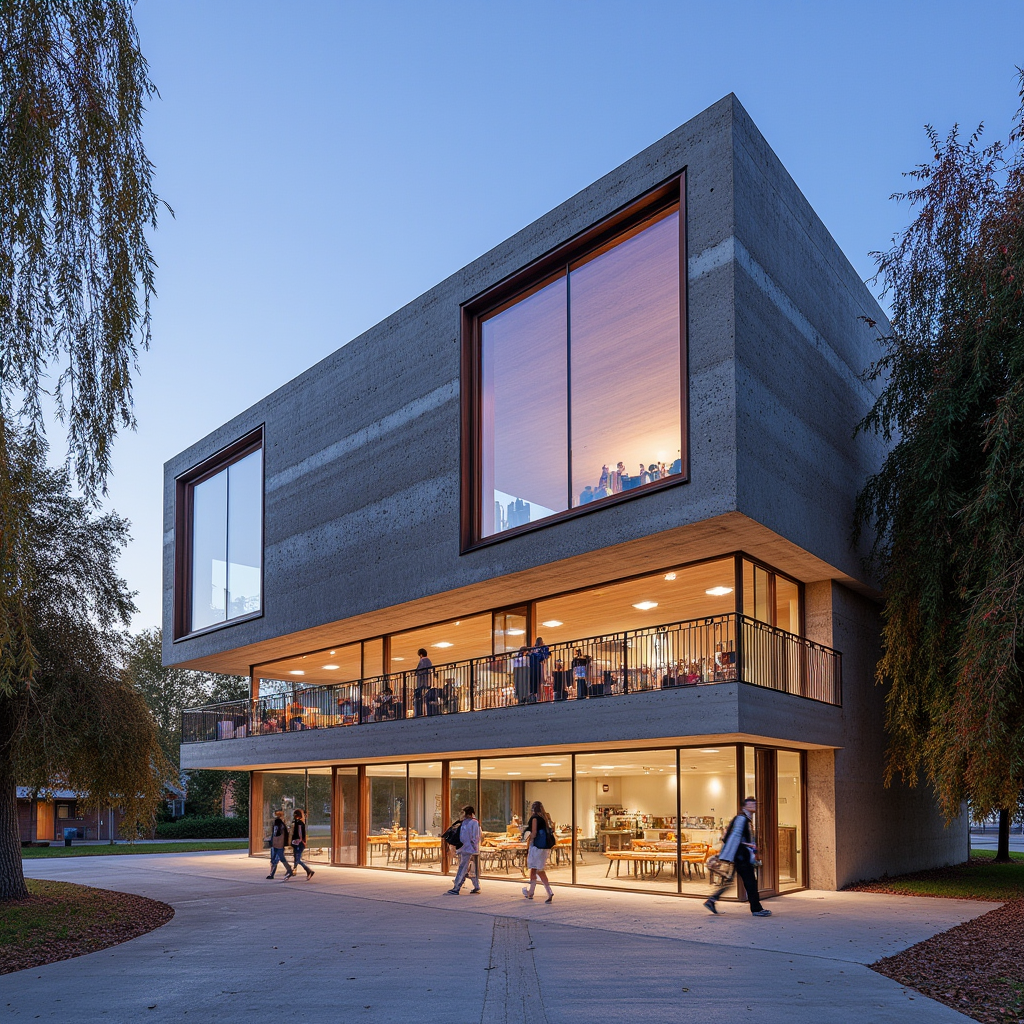
\includegraphics[width=0.12\textwidth]{Images/Results/Architect-A_Fixed-images/1-sketch_design/Met_lora_00001_.png}} & \href{https://github.com/matijspeeters/Thesis/blob/main/Images/Results/Architect-A_Fixed-images/1-sketch_design/Met_lora_00002_.png}{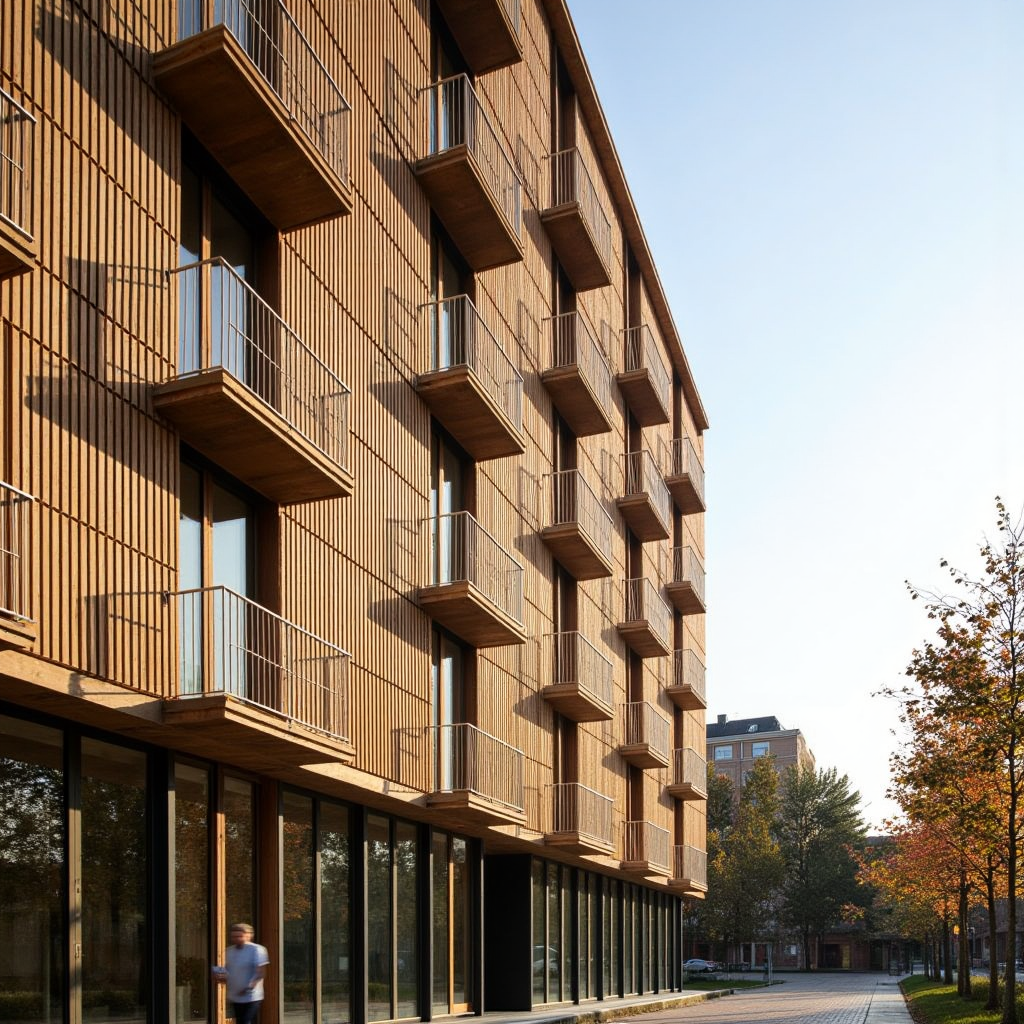
\includegraphics[width=0.12\textwidth]{Images/Results/Architect-A_Fixed-images/1-sketch_design/Met_lora_00002_.png}} &
    \href{https://github.com/matijspeeters/Thesis/blob/main/Images/Results/Architect-A_Fixed-images/1-sketch_design/Met_lora_00017_%20(2).png}{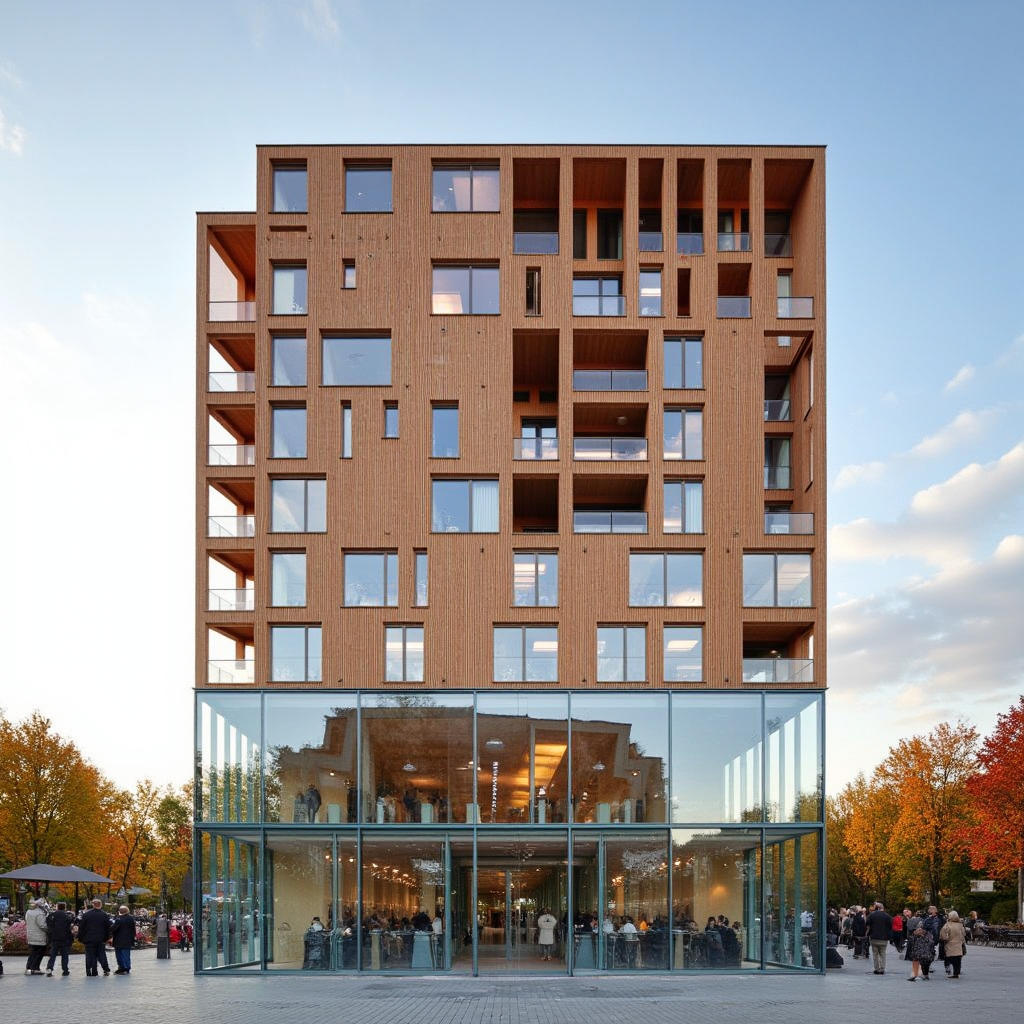
\includegraphics[width=0.12\textwidth]{Images/Results/Architect-A_Fixed-images/1-sketch_design/Met_lora_00017_ (2).png}} &
    \href{https://github.com/matijspeeters/Thesis/blob/main/Images/Results/Architect-A_Fixed-images/1-sketch_design/Met_lora_00029_.png}{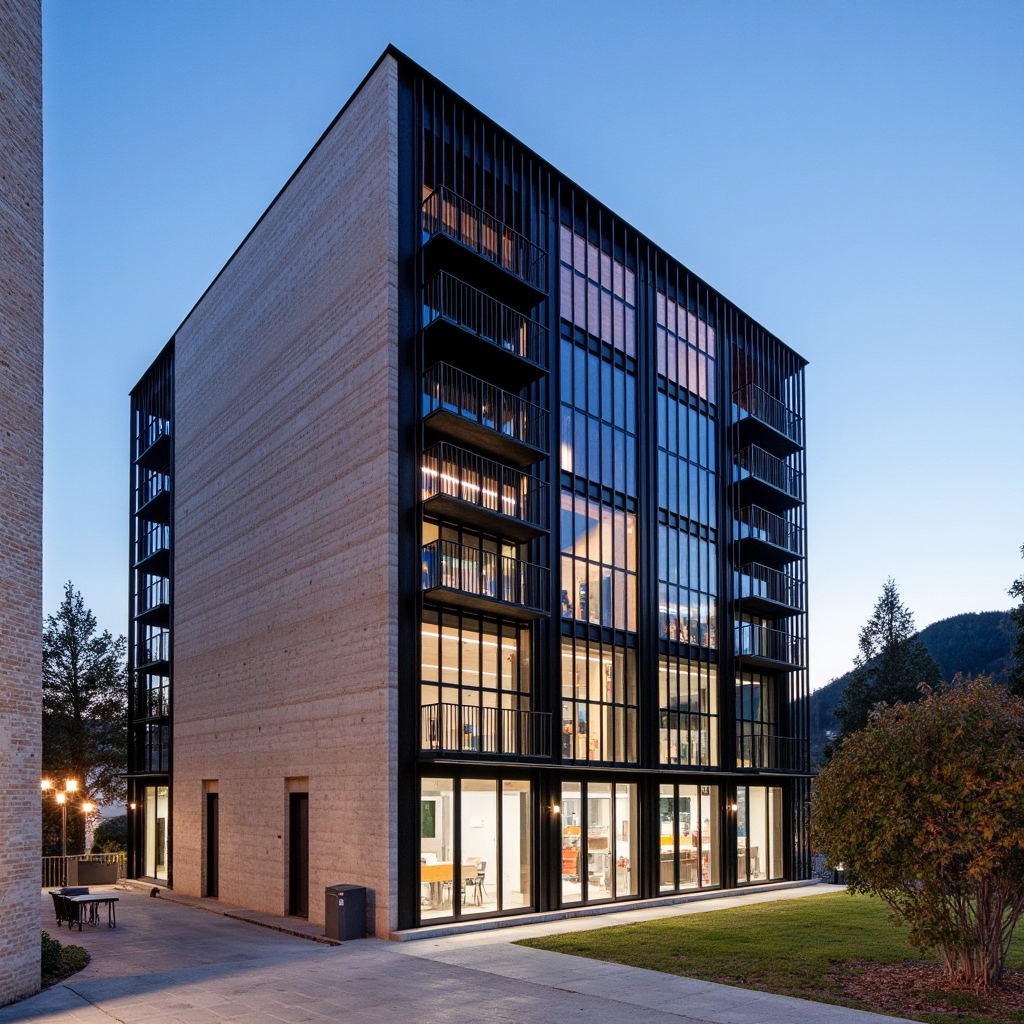
\includegraphics[width=0.12\textwidth]{Images/Results/Architect-A_Fixed-images/1-sketch_design/Met_lora_00029_.png}} &
    \href{https://github.com/matijspeeters/Thesis/blob/main/Images/Results/Architect-A_Fixed-images/1-sketch_design/Met_lora_00039_.png}{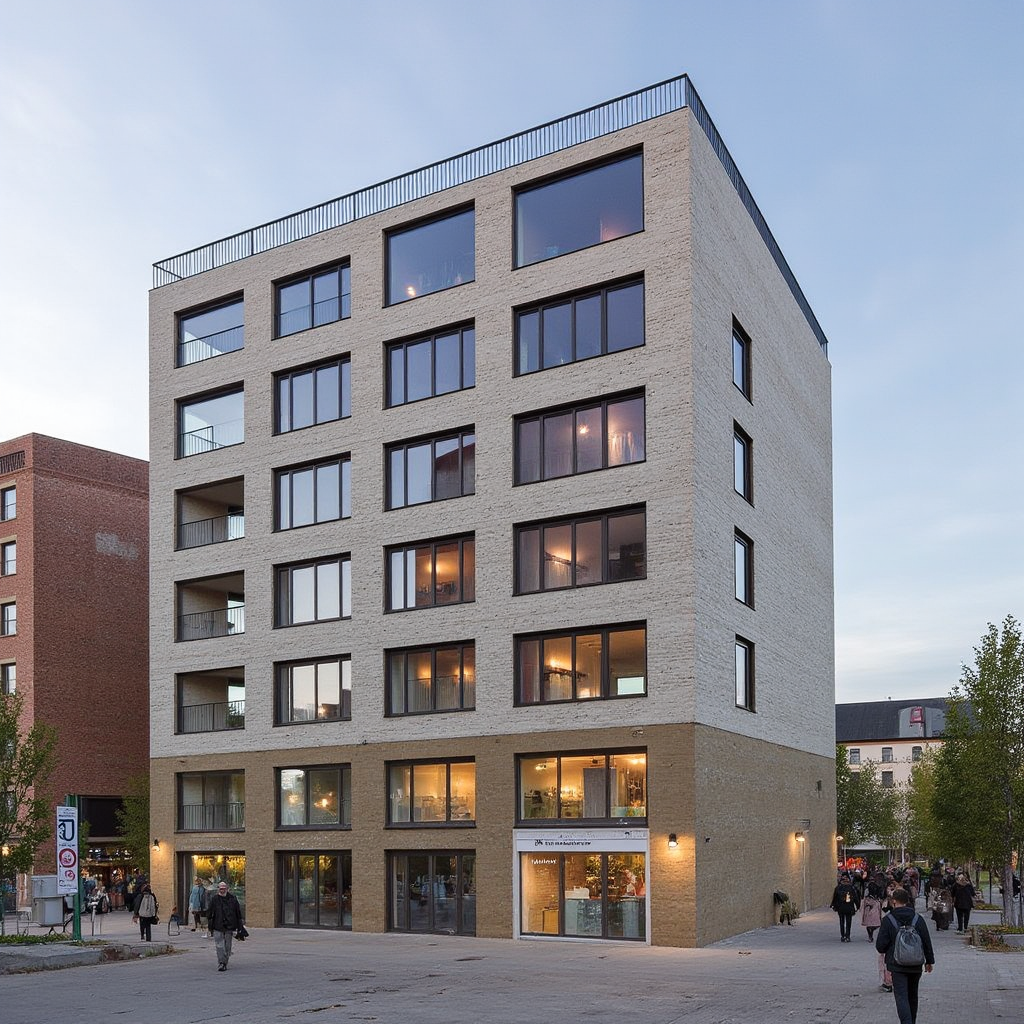
\includegraphics[width=0.12\textwidth]{Images/Results/Architect-A_Fixed-images/1-sketch_design/Met_lora_00039_.png}} &
    \href{https://github.com/matijspeeters/Thesis/blob/main/Images/Results/Architect-A_Fixed-images/1-sketch_design/Met_lora_00043_%20(1).png}{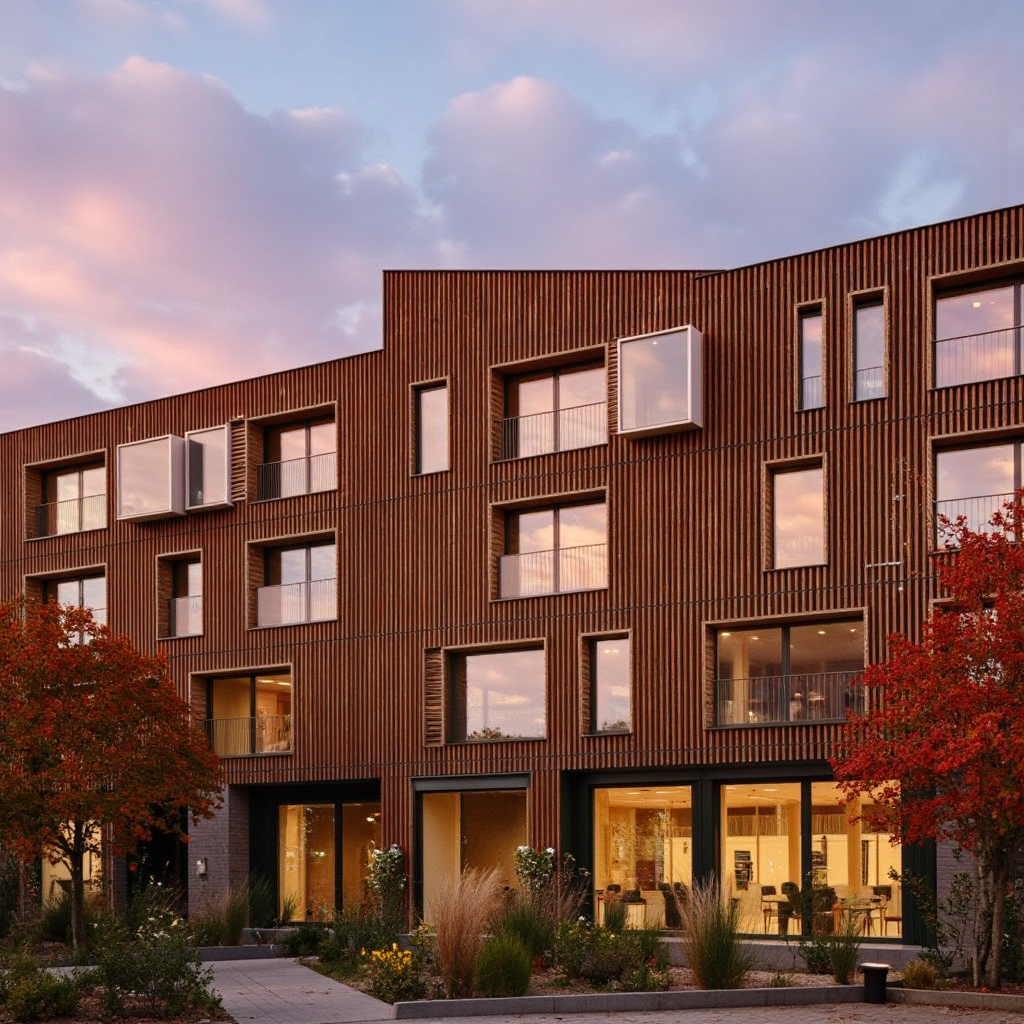
\includegraphics[width=0.12\textwidth]{Images/Results/Architect-A_Fixed-images/1-sketch_design/Met_lora_00043_ (1).png}} &
    \href{https://github.com/matijspeeters/Thesis/blob/main/Images/Results/Architect-A_Fixed-images/1-sketch_design/Met_lora_00058_.png}{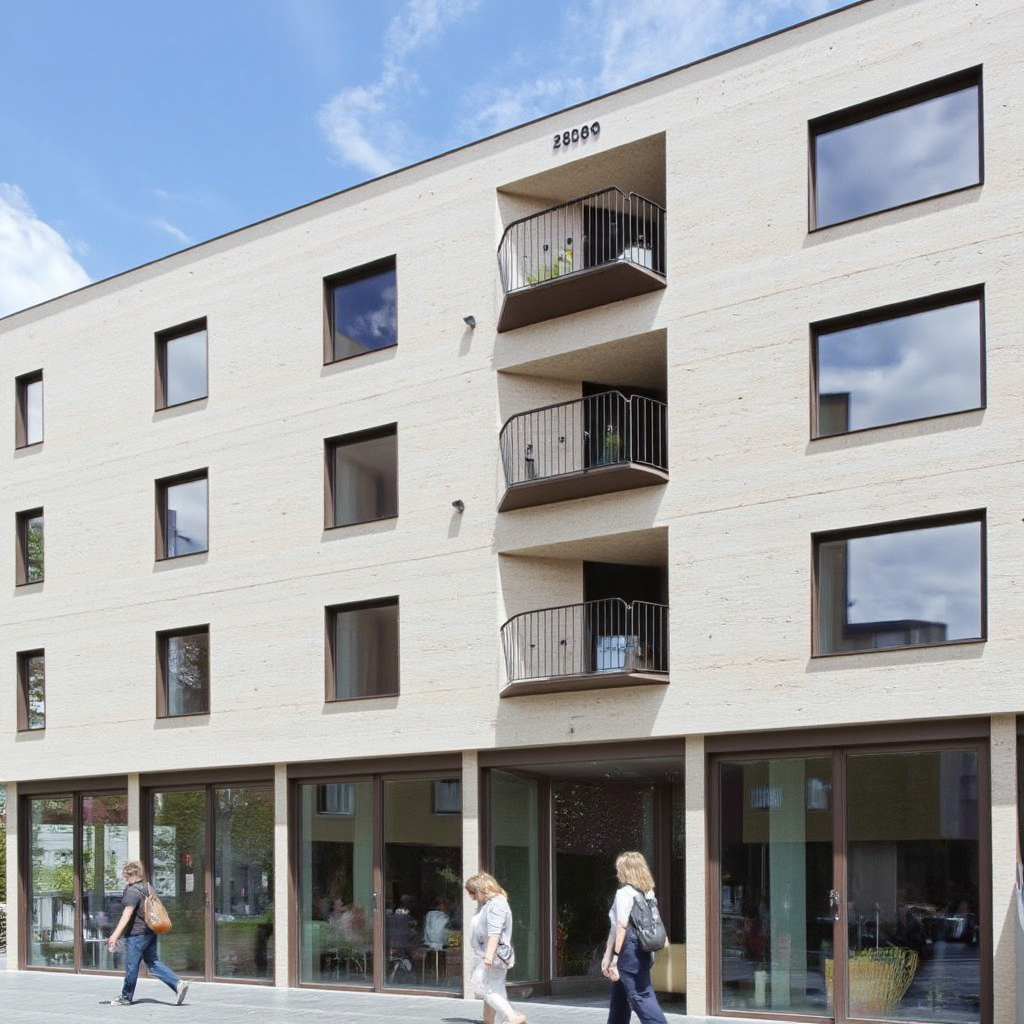
\includegraphics[width=0.12\textwidth]{Images/Results/Architect-A_Fixed-images/1-sketch_design/Met_lora_00058_.png}} \\

    \shortstack{\textbf{Without}\\\textbf{LoRA}} &
    \href{https://github.com/matijspeeters/Thesis/blob/main/Images/Results/Architect-A_Fixed-images/1-sketch_design/Zonder_lora_00001_.png}{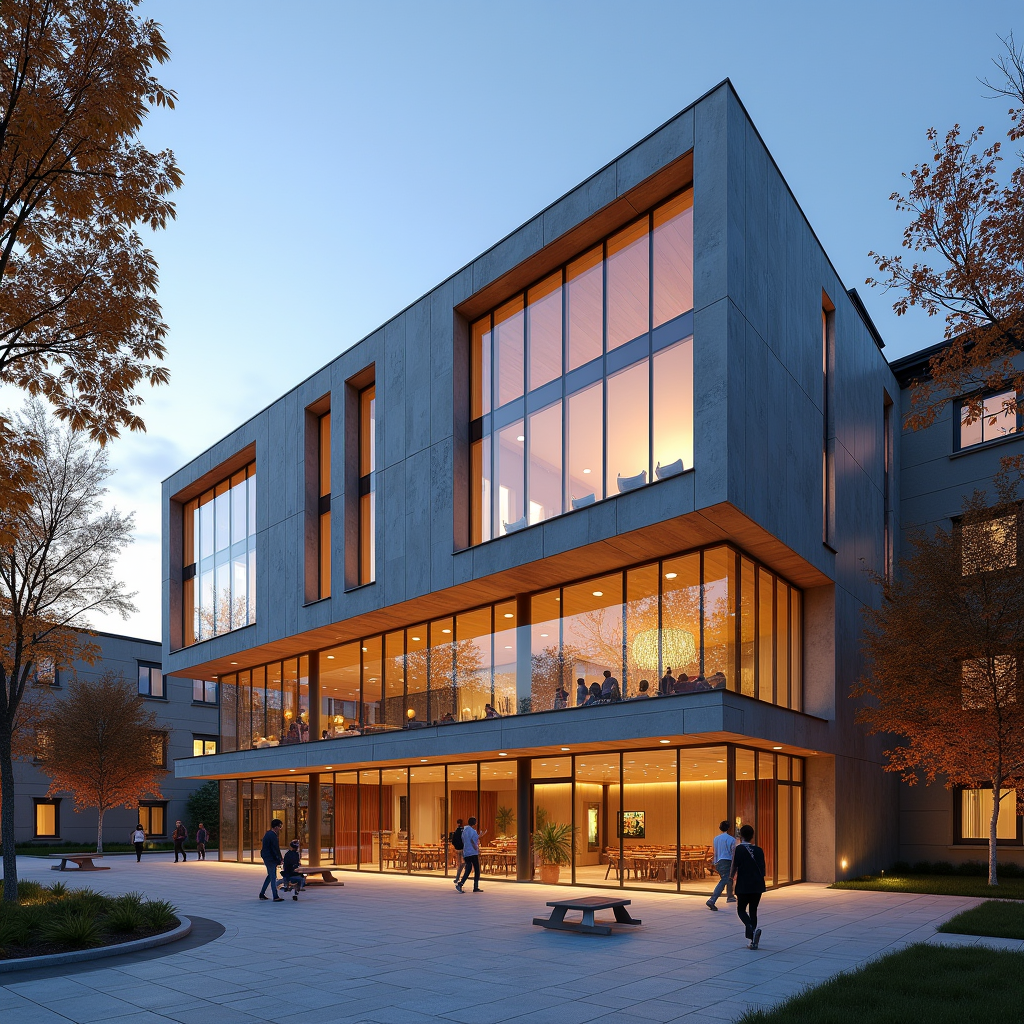
\includegraphics[width=0.12\textwidth]{Images/Results/Architect-A_Fixed-images/1-sketch_design/Zonder_lora_00001_.png}} &
    \href{https://github.com/matijspeeters/Thesis/blob/main/Images/Results/Architect-A_Fixed-images/1-sketch_design/Zonder_lora_00002_.png}{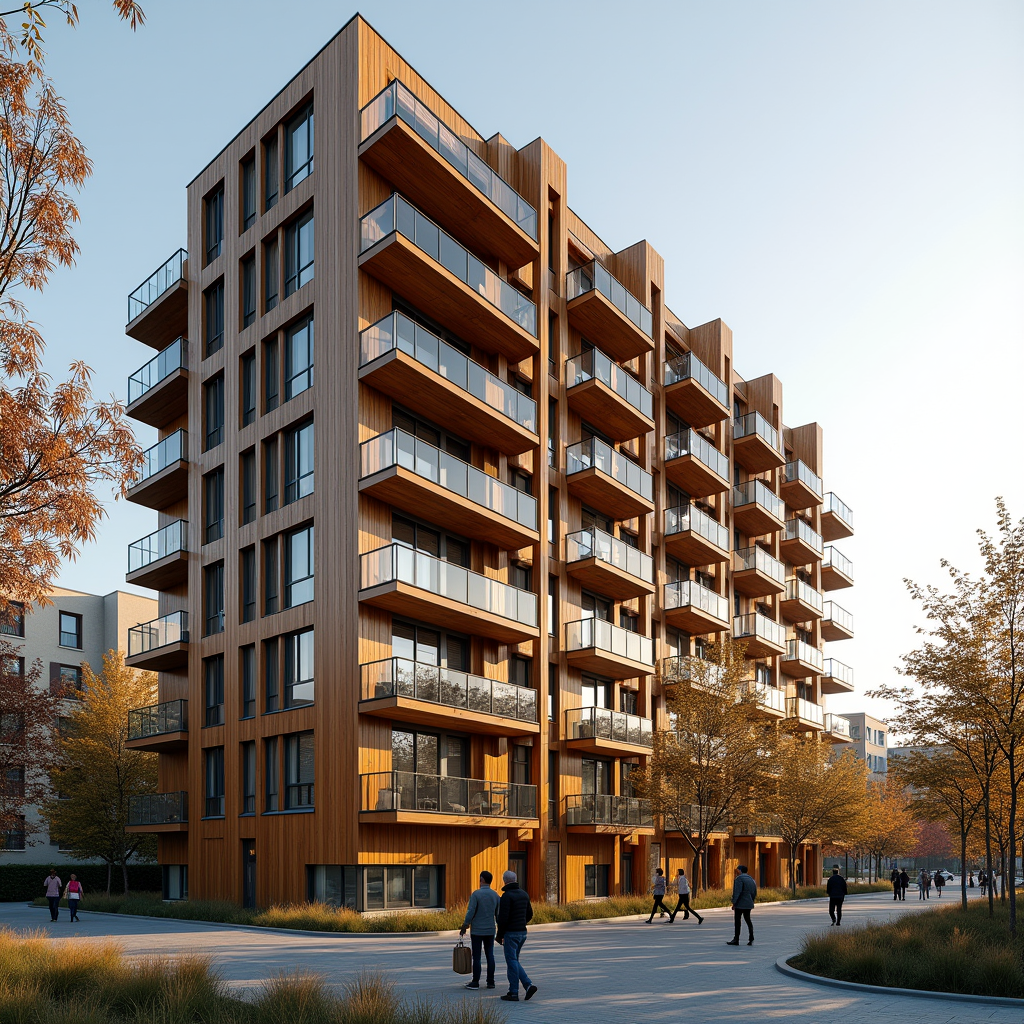
\includegraphics[width=0.12\textwidth]{Images/Results/Architect-A_Fixed-images/1-sketch_design/Zonder_lora_00002_.png}} &
    \href{https://github.com/matijspeeters/Thesis/blob/main/Images/Results/Architect-A_Fixed-images/1-sketch_design/Zonder_lora_00017_%20(1).png}{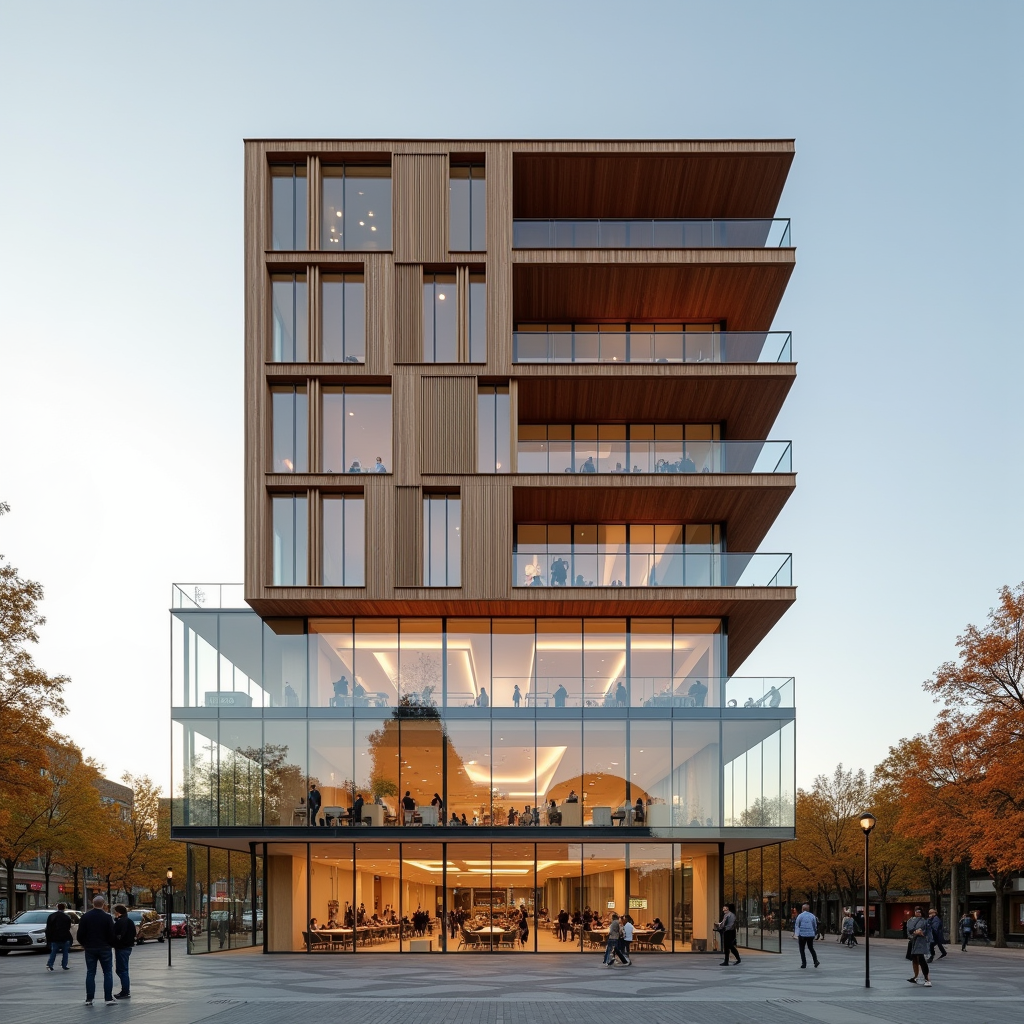
\includegraphics[width=0.12\textwidth]{Images/Results/Architect-A_Fixed-images/1-sketch_design/Zonder_lora_00017_ (1).png}} &
    \href{https://github.com/matijspeeters/Thesis/blob/main/Images/Results/Architect-A_Fixed-images/1-sketch_design/Zonder_lora_00029_.png}{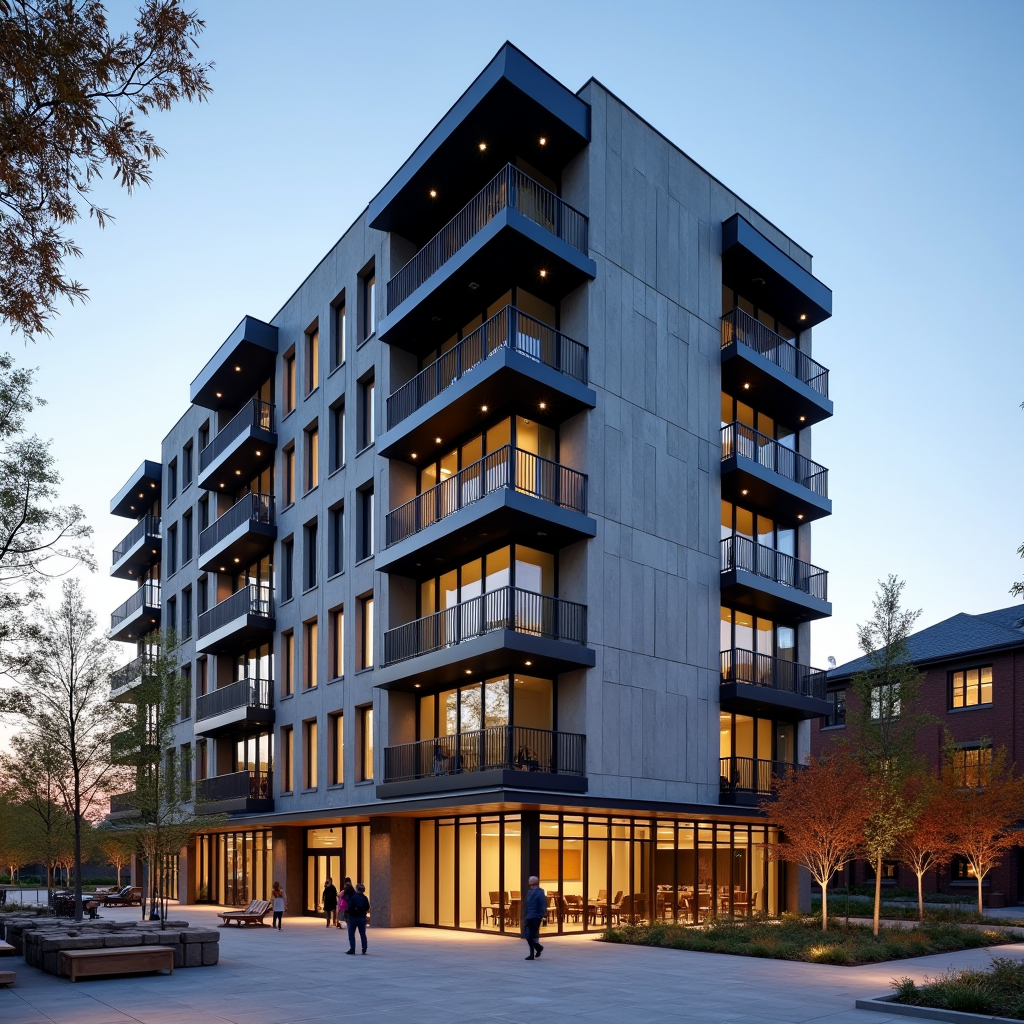
\includegraphics[width=0.12\textwidth]{Images/Results/Architect-A_Fixed-images/1-sketch_design/Zonder_lora_00029_.png}} &
    \href{https://github.com/matijspeeters/Thesis/blob/main/Images/Results/Architect-A_Fixed-images/1-sketch_design/Zonder_lora_00039_.png}{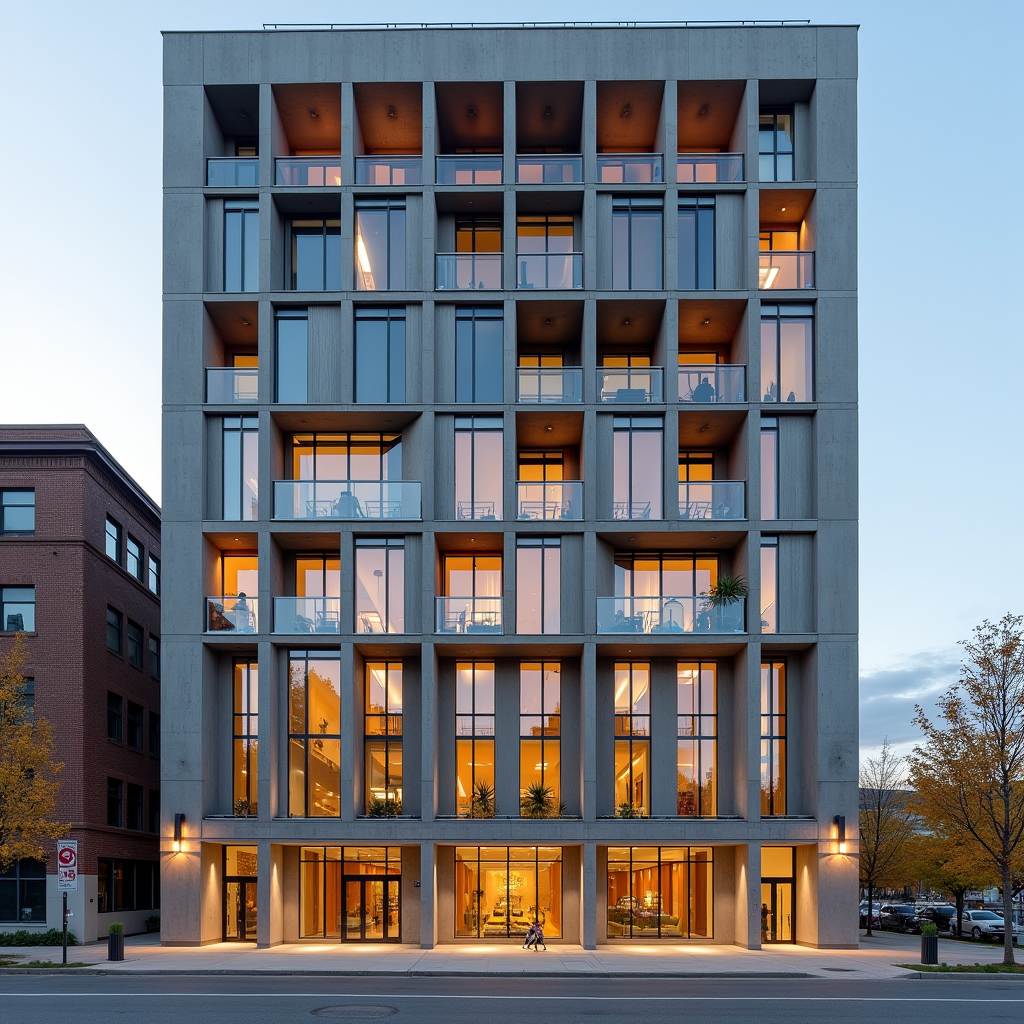
\includegraphics[width=0.12\textwidth]{Images/Results/Architect-A_Fixed-images/1-sketch_design/Zonder_lora_00039_.png}} &
    \href{https://github.com/matijspeeters/Thesis/blob/main/Images/Results/Architect-A_Fixed-images/1-sketch_design/Zonder_lora_00043_%20(1).png}{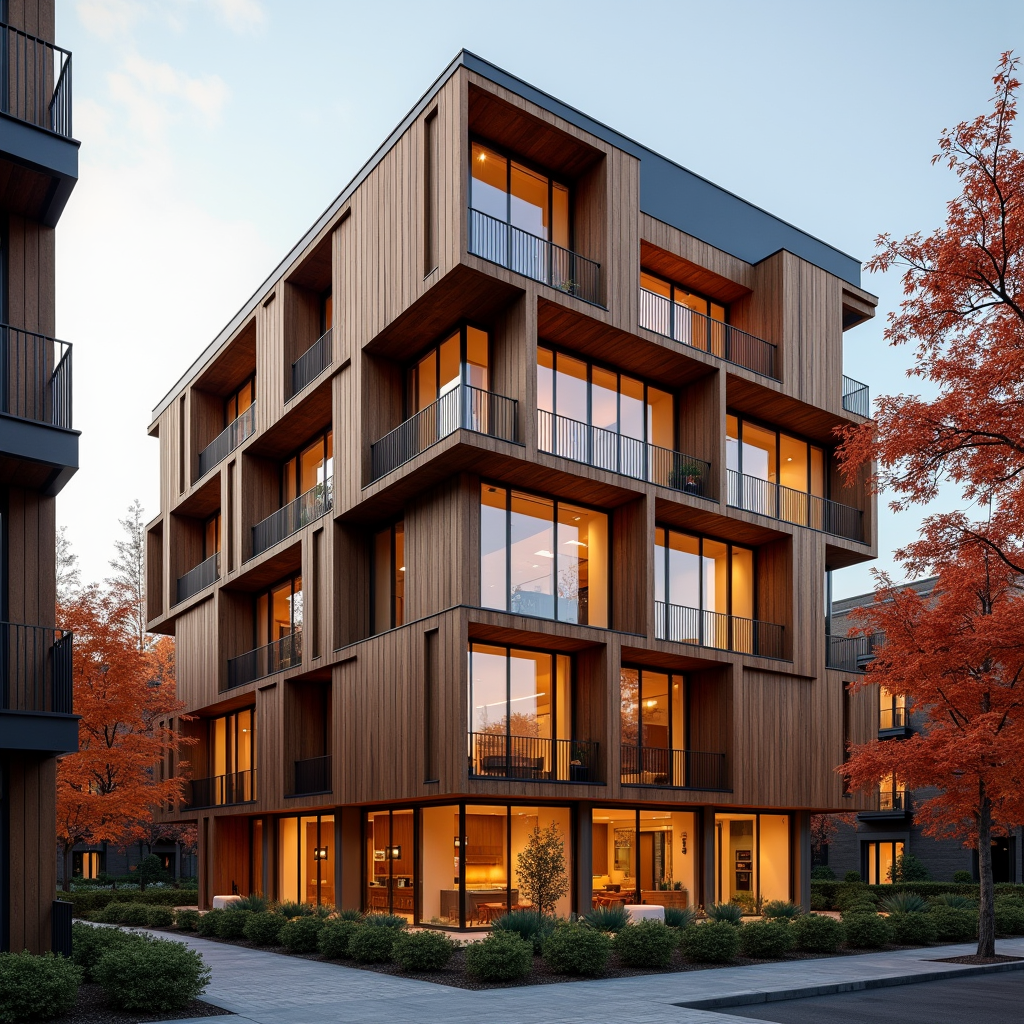
\includegraphics[width=0.12\textwidth]{Images/Results/Architect-A_Fixed-images/1-sketch_design/Zonder_lora_00043_ (1).png}} &
    \href{https://github.com/matijspeeters/Thesis/blob/main/Images/Results/Architect-A_Fixed-images/1-sketch_design/Zonder_lora_00058_.png}{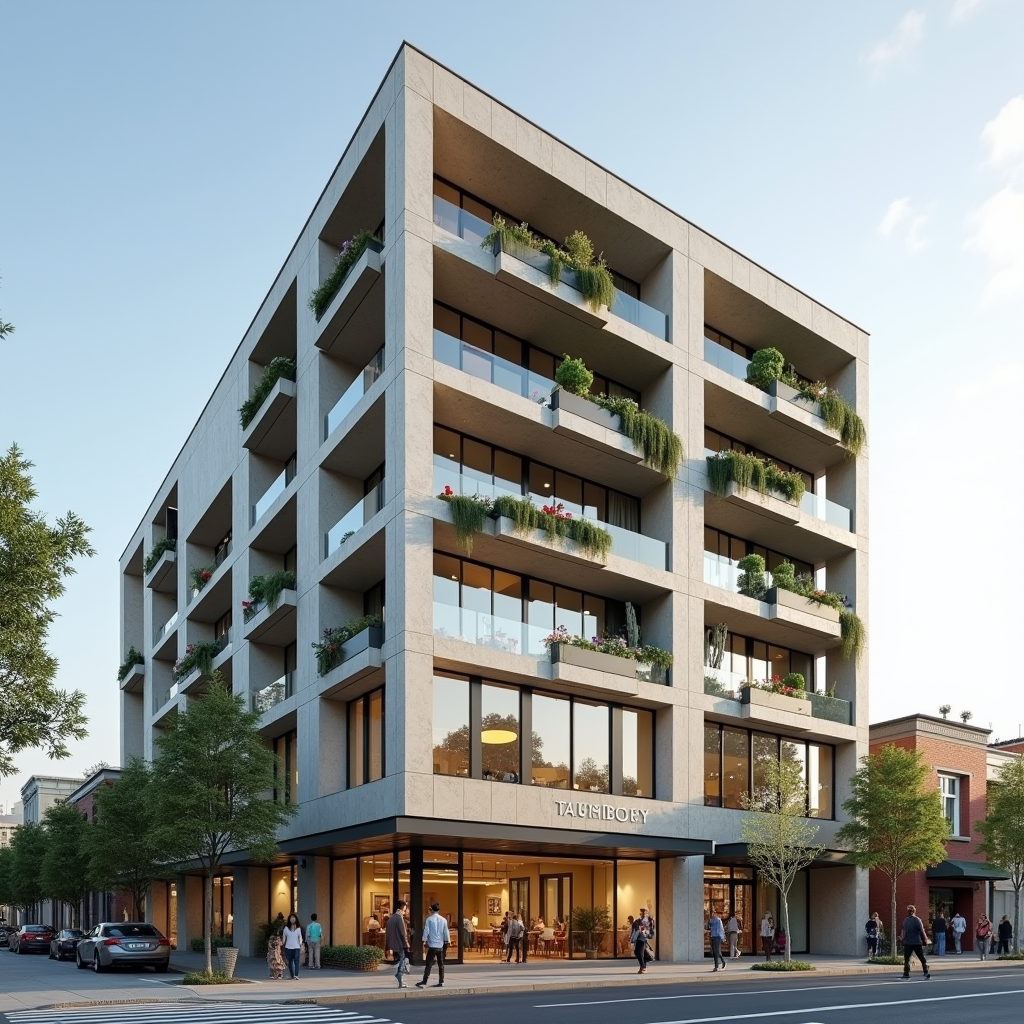
\includegraphics[width=0.12\textwidth]{Images/Results/Architect-A_Fixed-images/1-sketch_design/Zonder_lora_00058_.png}} \\
  \end{tabular}
  }
  \caption{Starting images in the sketch design phase of architect A.}
  \label{fig:horizontal-lora-comparison}
\end{figure}
\subsubsection{Selected starting image}
Architect A selected the image in figure \ref{fig:A-sketch-selected}, which was generated with the \textbf{3D-effect} and \textbf{Geleding} models. His reasons were two-fold: the 'warm facade cladding' and 'a clear connection to the ground level'.
\begin{figure}[H]
    \centering
    \href{https://github.com/matijspeeters/Thesis/blob/main/Images/Results/Architect-A_Fixed-images/1-sketch_design/Met_lora_00043_%20(1).png}{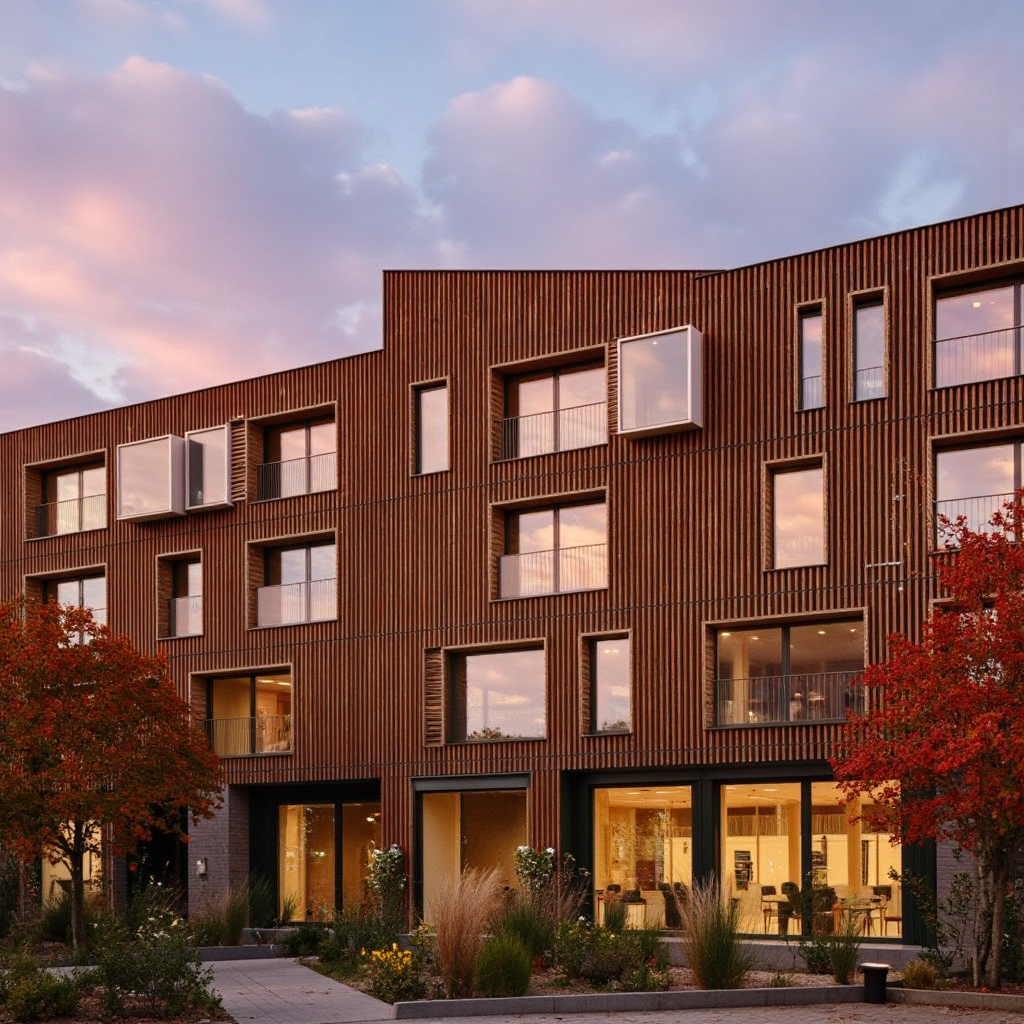
\includegraphics[width=0.3\linewidth]{Images/Results/Architect-A_Fixed-images/1-sketch_design/Met_lora_00043_ (1).png}}
    \caption{Architect A's selected starting image for the sketch design phase.}
    \label{fig:A-sketch-selected}
\end{figure}
\subsubsection{Preferred generated images}
Architect A selected 3 preferred images (figure \ref{fig:A-sketch-favourite}) among the generated images during the sketch design phase. In his opinion, image 1 and 2 shared a 'combination of old and new'. The building in image 3 was 'playing with volumes, rather than referring to something'. It 'introduces a very strong gesture' and 'interacts with nature'.
\begin{figure}[H]
    \centering
    \begin{tabular}{ccc}
         \href{https://github.com/matijspeeters/Thesis/blob/main/Images/Results/Architect%20A/1.%20sketch%20phase/Met_lora_00126_.png}{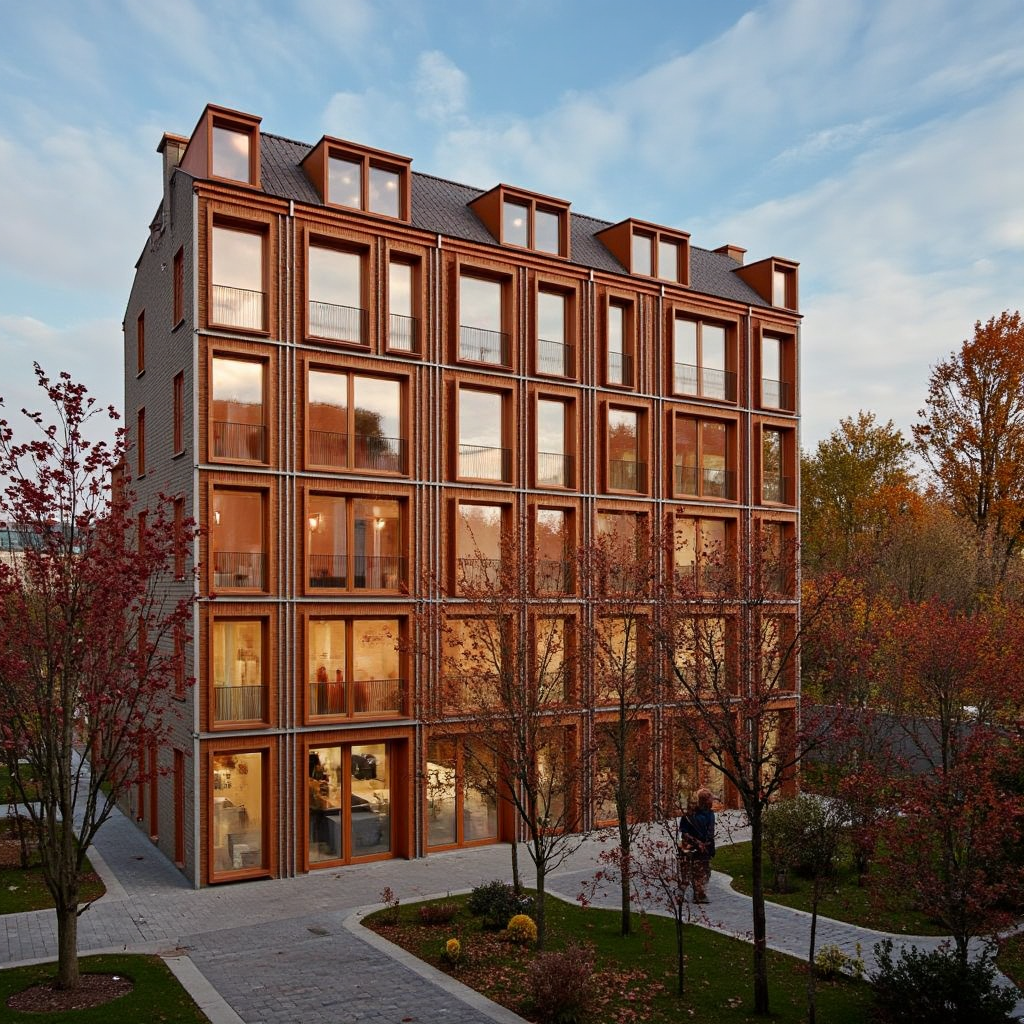
\includegraphics[width=0.3\linewidth]{Images/Results/Architect A/1. sketch phase/Met_lora_00126_.png}}
         & \href{https://github.com/matijspeeters/Thesis/blob/main/Images/Results/Architect%20A/1.%20sketch%20phase/Met_lora_00139_.png}{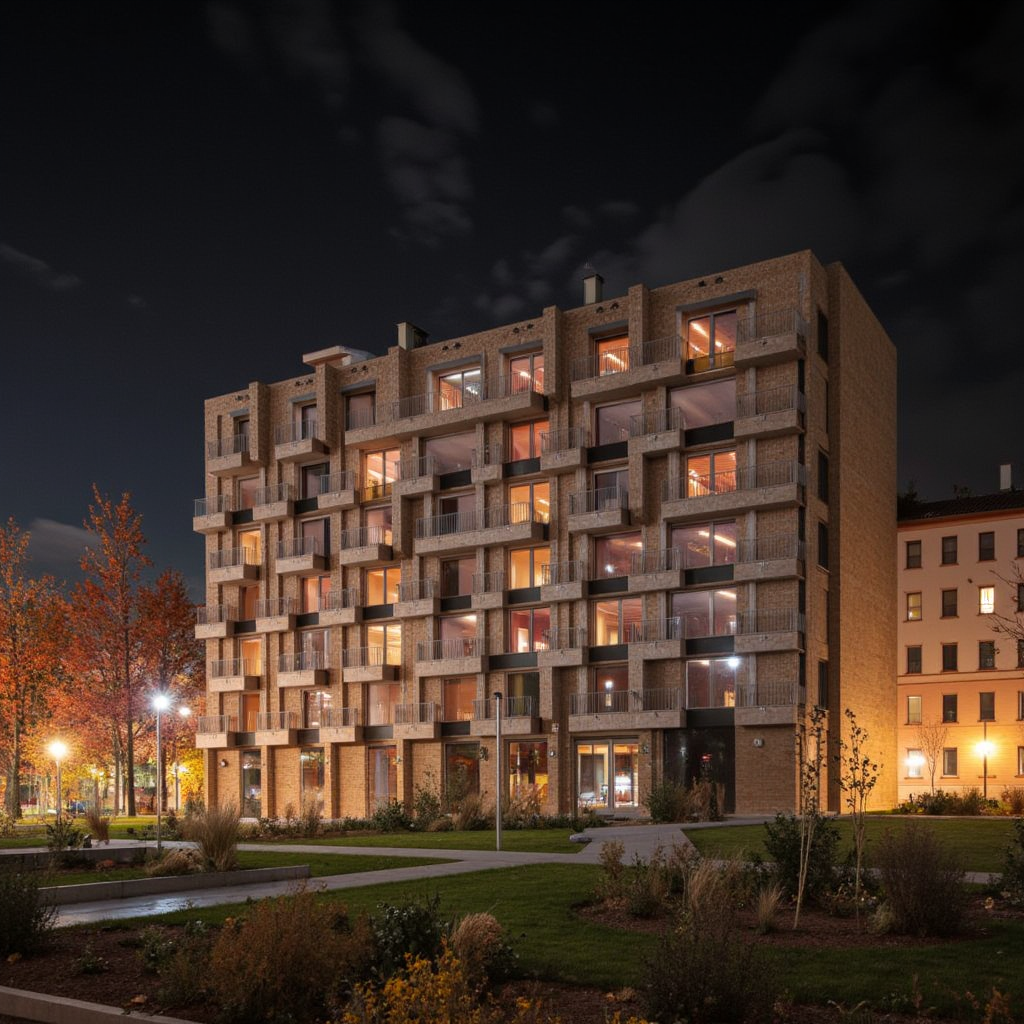
\includegraphics[width=0.3\linewidth]{Images/Results/Architect A/1. sketch phase/Met_lora_00139_.png}}
         & \href{https://github.com/matijspeeters/Thesis/blob/main/Images/Results/Architect%20A/1.%20sketch%20phase/Zonder_lora_00144_.png}{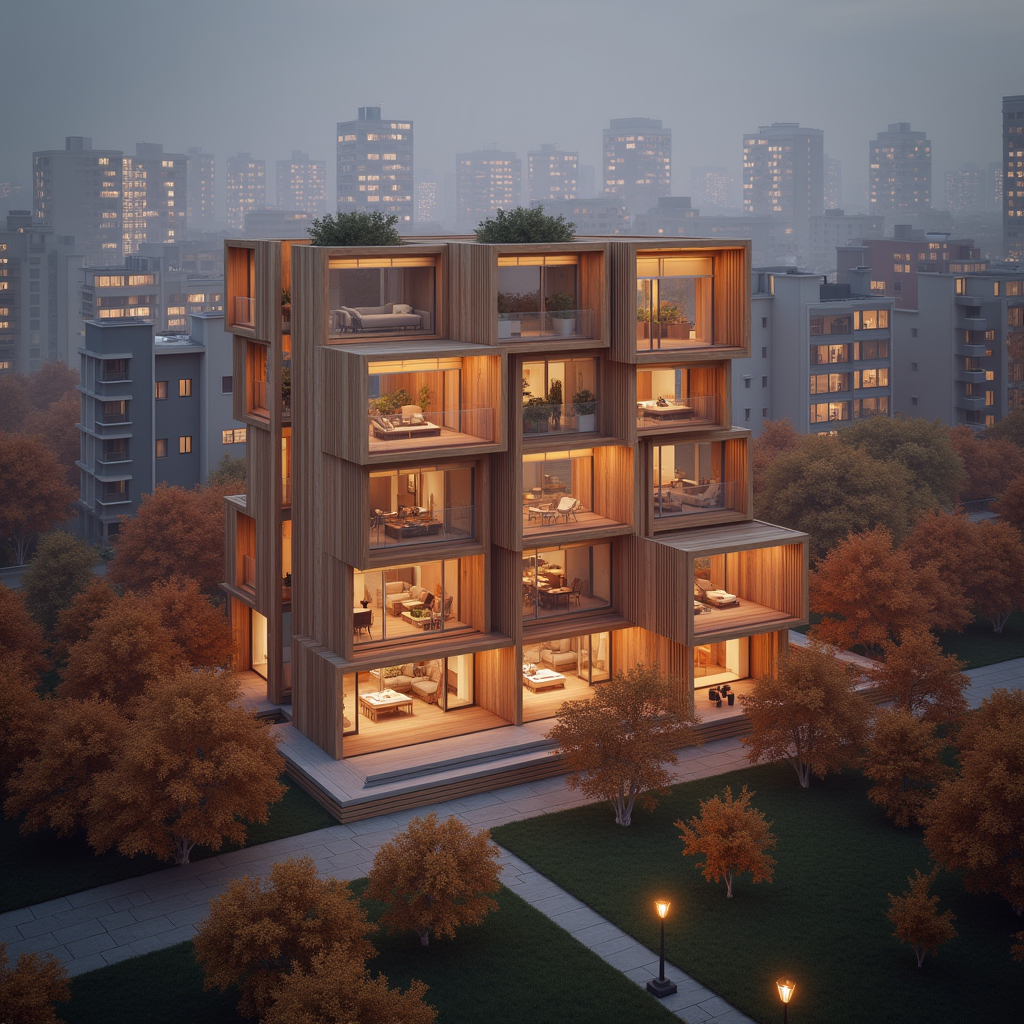
\includegraphics[width=0.3\linewidth]{Images/Results/Architect A/1. sketch phase/Zonder_lora_00144_.png}}\\
         \textit{(1)} & \textit{(2)} & \textit{(3)}
    \end{tabular}
    \caption{Architect A's favourite images in the sketch design phase.}
    \label{fig:A-sketch-favourite}
\end{figure}
\subsection{Preliminary design phase}
\subsubsection{Starting images}
\begin{figure}[H]
  \centering
  {\footnotesize
  \renewcommand{\arraystretch}{1.1}
  \setlength{\tabcolsep}{4pt}
  \begin{tabular}{c c c c c c c c}
    & \shortstack{\textbf{Stamp-}\\\textbf{beton}} 
    & \shortstack{\textbf{3D-}\\\textbf{effect}} 
    & \textbf{Geleding} 
    & \shortstack{\textbf{Stampbeton}\\ \textbf{\& 3D-effect}} 
    & \shortstack{\textbf{Stampbeton}\\ \textbf{\& Geleding}} 
    & \shortstack{\textbf{3D-effect} \&\\ \textbf{Geleding}} 
    & \shortstack{\textbf{Stampbeton,}\\\textbf{3D-effect \&}\\\textbf{Geleding}} \\

    \shortstack{\textbf{With}\\\textbf{LoRA}} & 
    \href{https://github.com/matijspeeters/Thesis/blob/main/Images/Results/Architect-A_Fixed-images/2-preliminary_design/Met_lora_00059_%20(1).png}{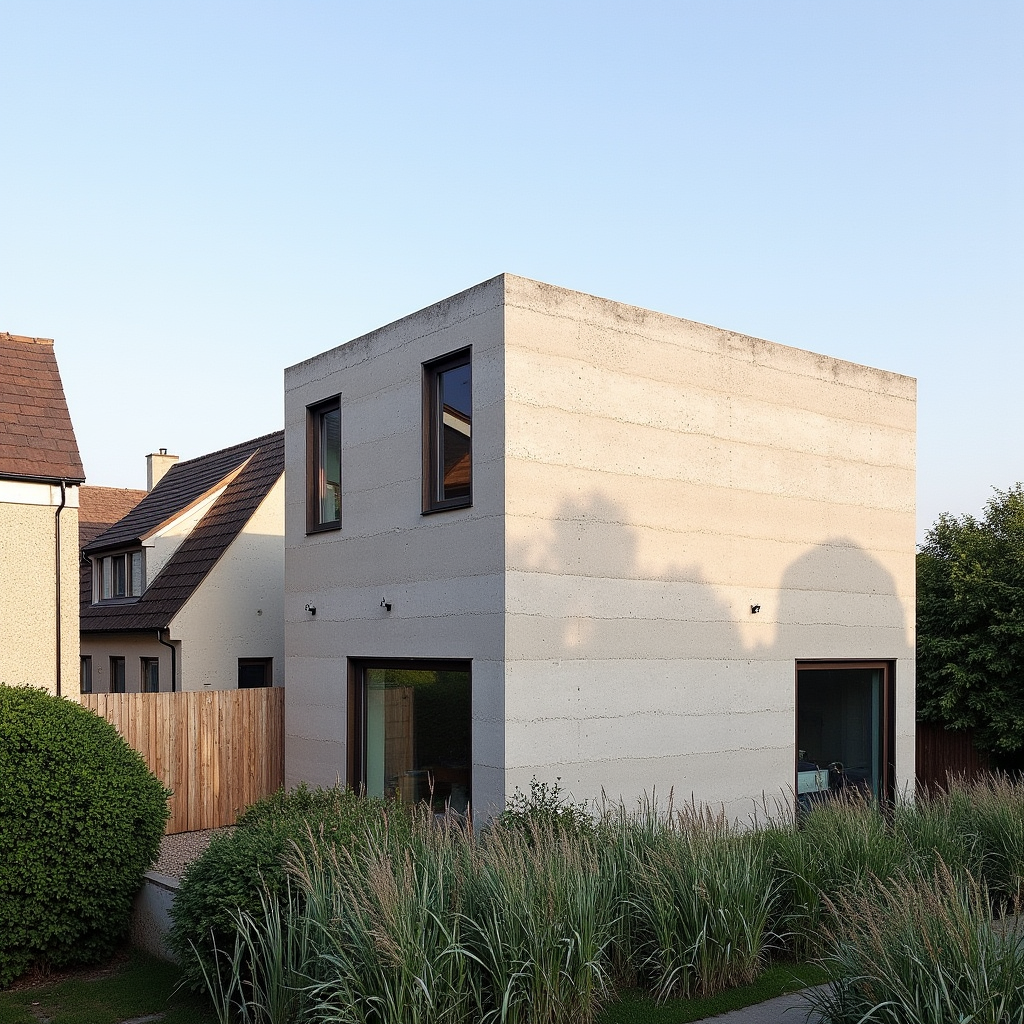
\includegraphics[width=0.12\textwidth]{Images/Results/Architect-A_Fixed-images/2-preliminary_design/Met_lora_00059_ (1).png}} & 
    \href{https://github.com/matijspeeters/Thesis/blob/main/Images/Results/Architect-A_Fixed-images/2-preliminary_design/Met_lora_00061_.png}{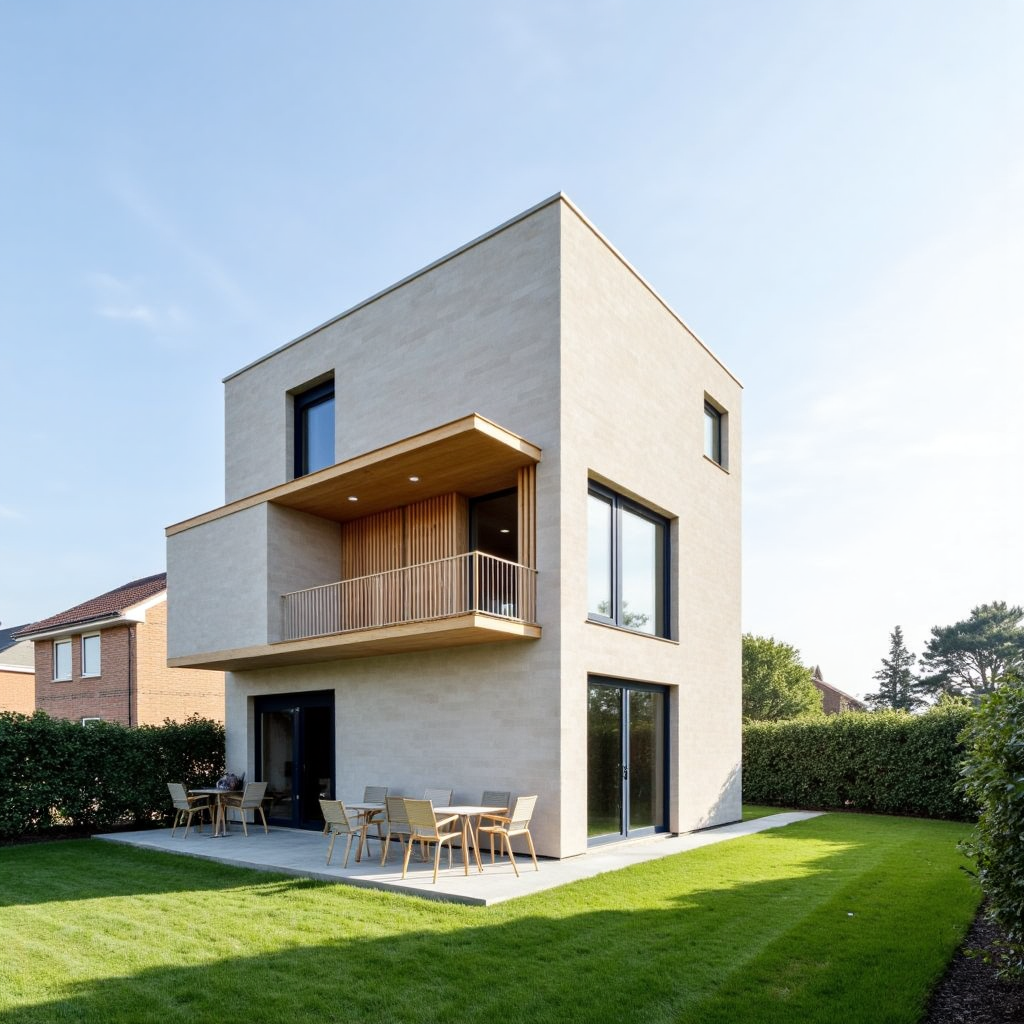
\includegraphics[width=0.12\textwidth]{Images/Results/Architect-A_Fixed-images/2-preliminary_design/Met_lora_00061_.png}} &
    \href{https://github.com/matijspeeters/Thesis/blob/main/Images/Results/Architect-A_Fixed-images/2-preliminary_design/Met_lora_00069_%20(1).png}{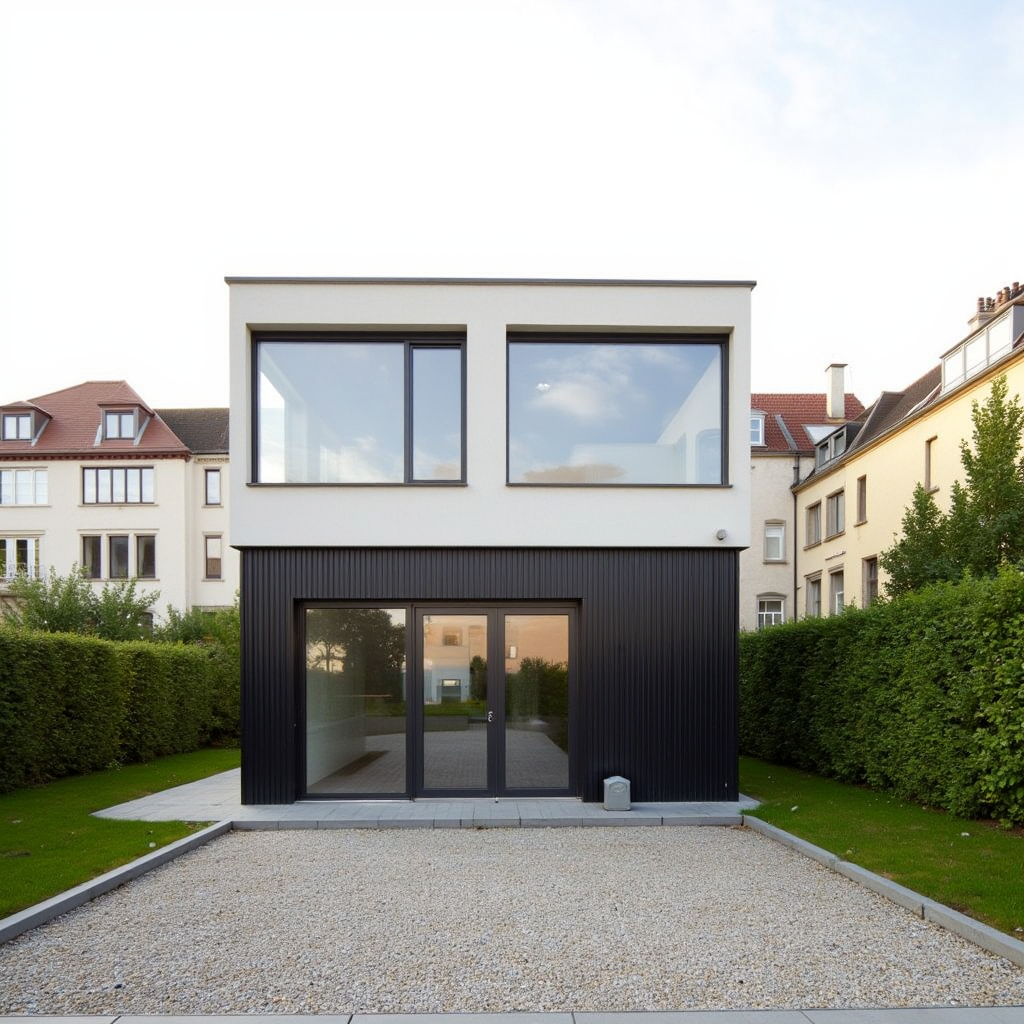
\includegraphics[width=0.12\textwidth]{Images/Results/Architect-A_Fixed-images/2-preliminary_design/Met_lora_00069_ (1).png}} &
    \href{https://github.com/matijspeeters/Thesis/blob/main/Images/Results/Architect-A_Fixed-images/2-preliminary_design/Met_lora_00080_.png}{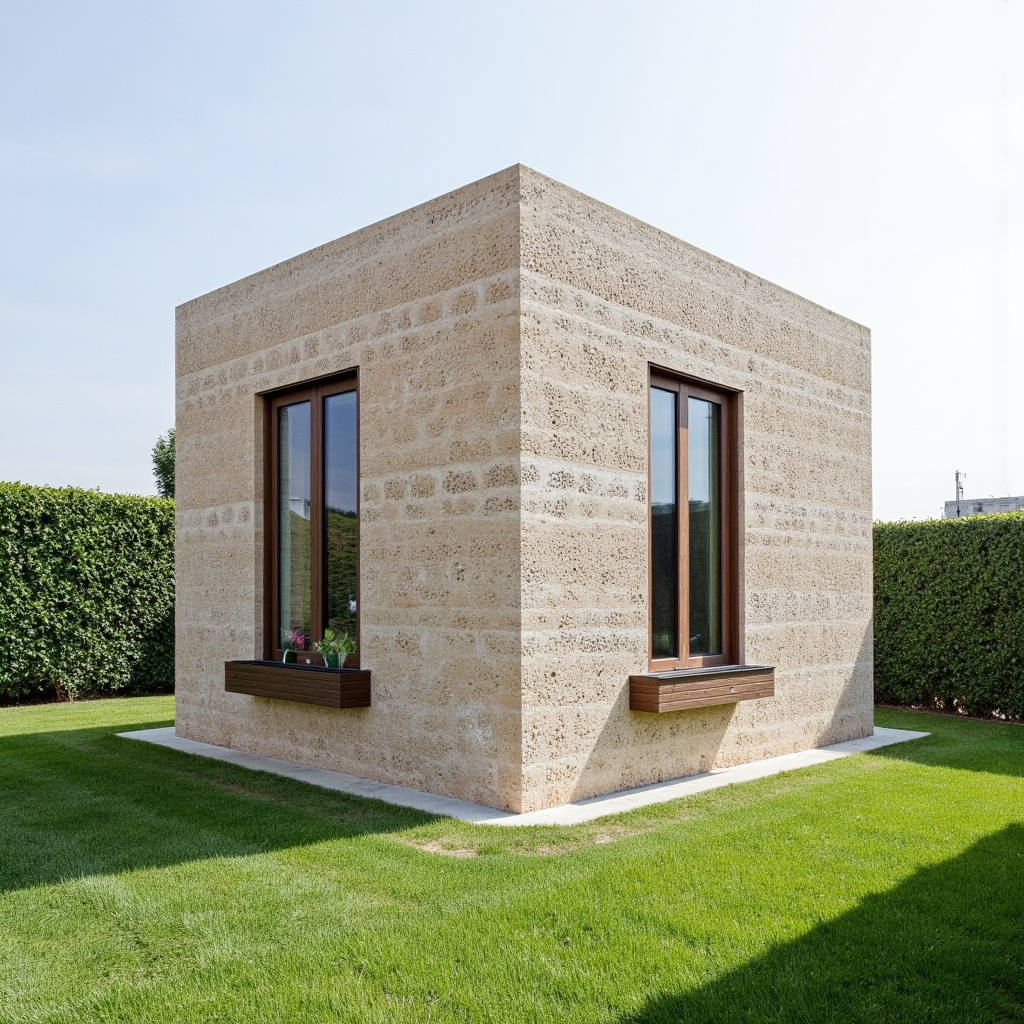
\includegraphics[width=0.12\textwidth]{Images/Results/Architect-A_Fixed-images/2-preliminary_design/Met_lora_00080_.png}} &
    \href{https://github.com/matijspeeters/Thesis/blob/main/Images/Results/Architect-A_Fixed-images/2-preliminary_design/Met_lora_00089_.png}{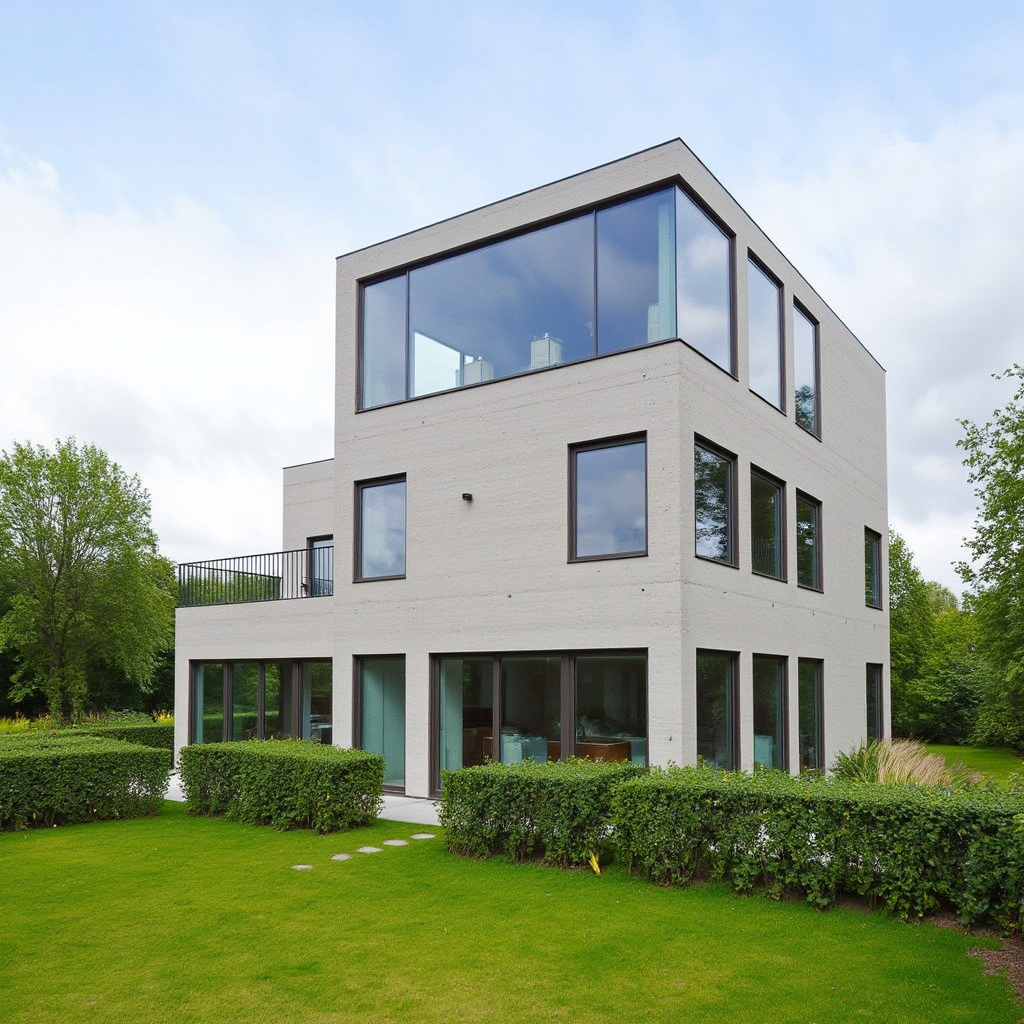
\includegraphics[width=0.12\textwidth]{Images/Results/Architect-A_Fixed-images/2-preliminary_design/Met_lora_00089_.png}} &
    \href{https://github.com/matijspeeters/Thesis/blob/main/Images/Results/Architect-A_Fixed-images/2-preliminary_design/Met_lora_00091_.png}{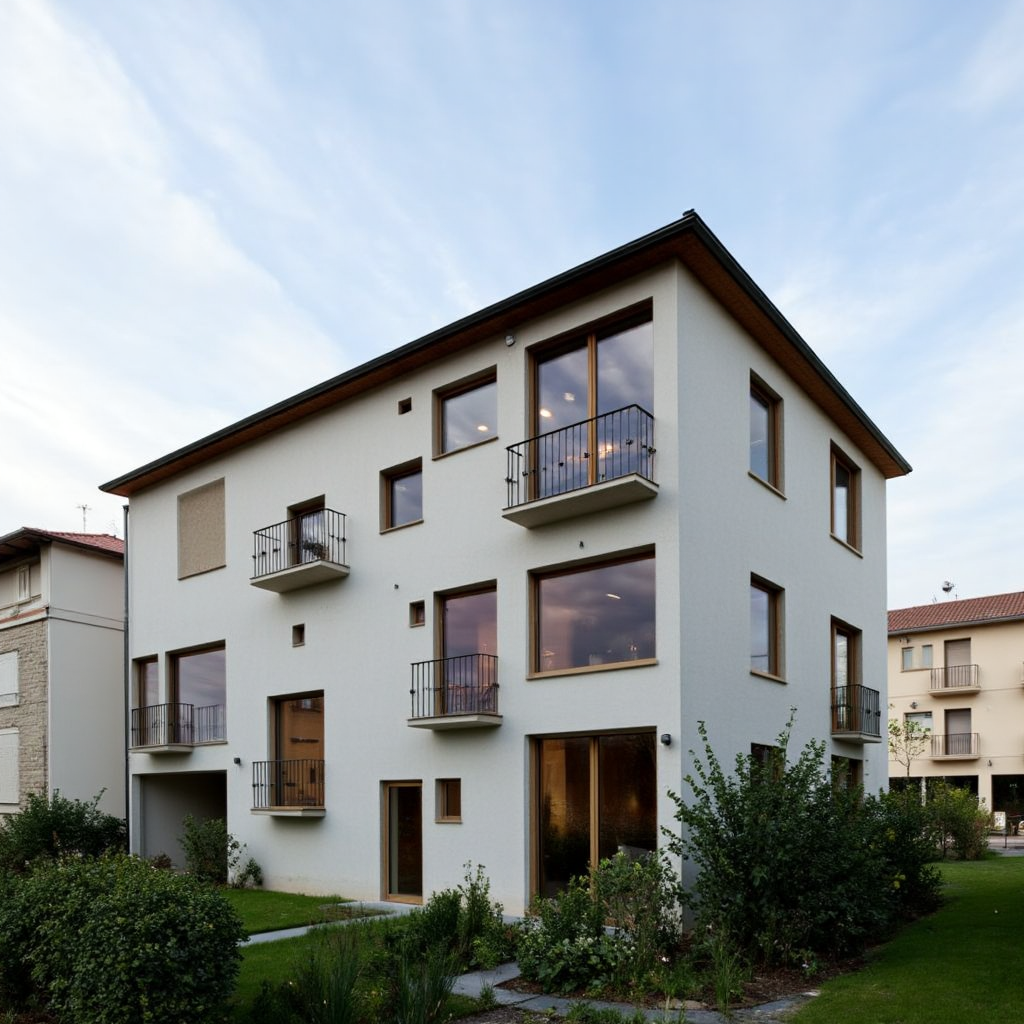
\includegraphics[width=0.12\textwidth]{Images/Results/Architect-A_Fixed-images/2-preliminary_design/Met_lora_00091_.png}} &
    \href{https://github.com/matijspeeters/Thesis/blob/main/Images/Results/Architect-A_Fixed-images/2-preliminary_design/Met_lora_00095_.png}{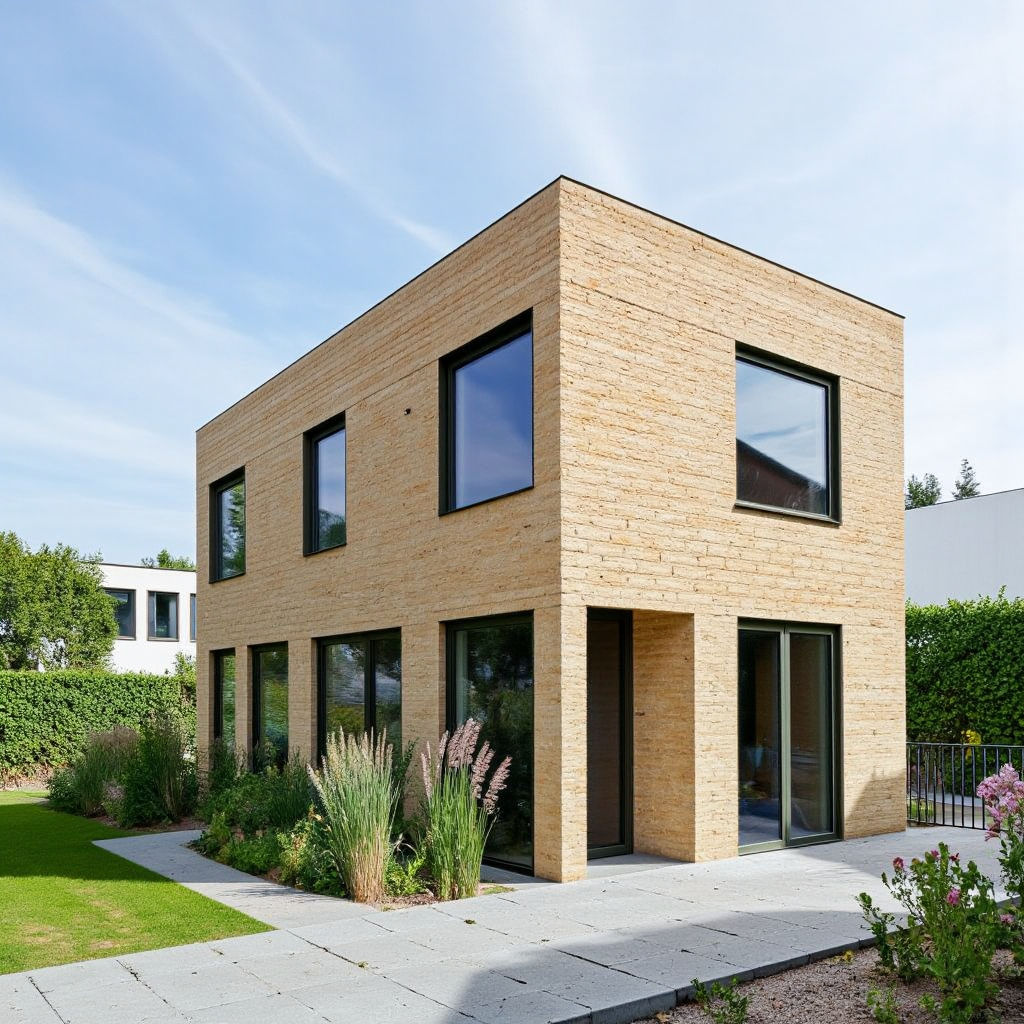
\includegraphics[width=0.12\textwidth]{Images/Results/Architect-A_Fixed-images/2-preliminary_design/Met_lora_00095_.png}} \\

    \shortstack{\textbf{Without}\\\textbf{LoRA}} &
    \href{https://github.com/matijspeeters/Thesis/blob/main/Images/Results/Architect-A_Fixed-images/2-preliminary_design/Zonder_lora_00059_%20(1).png}{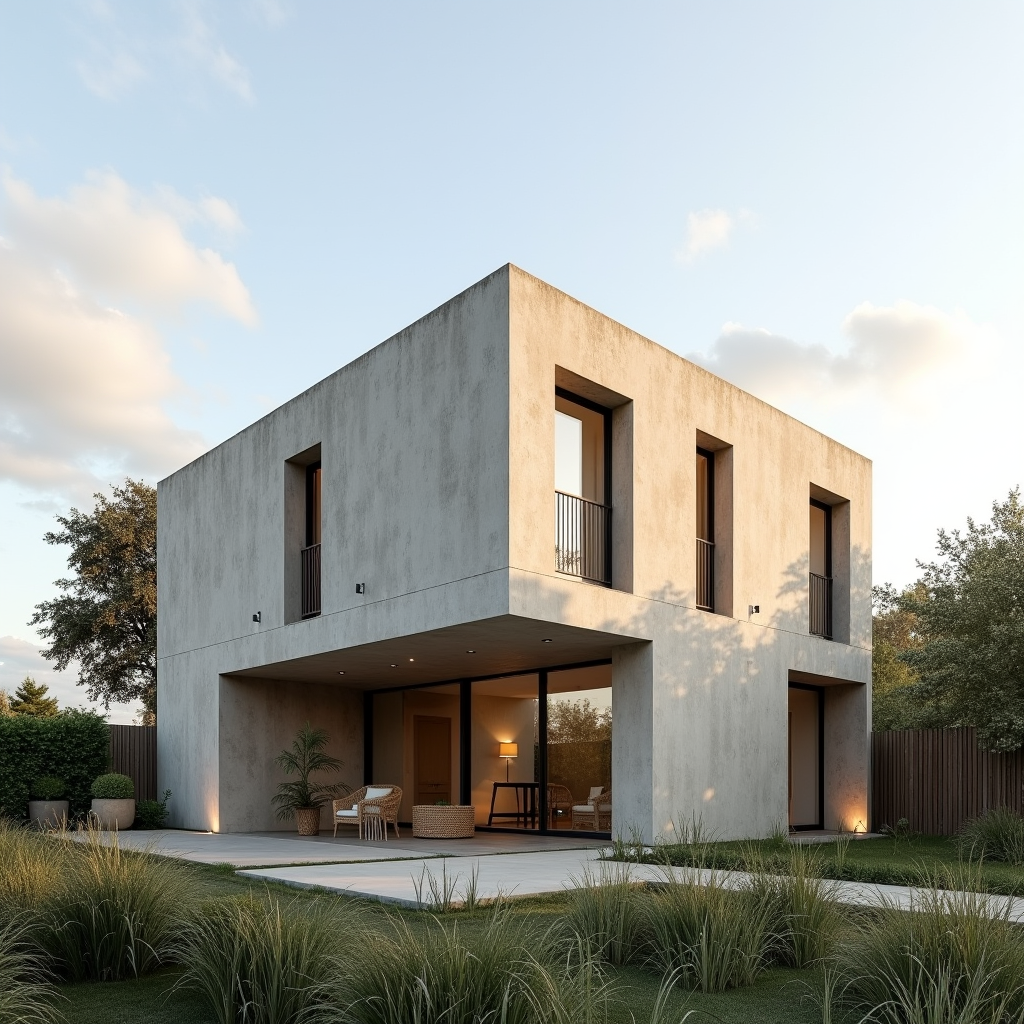
\includegraphics[width=0.12\textwidth]{Images/Results/Architect-A_Fixed-images/2-preliminary_design/Zonder_lora_00059_ (1).png}} &
    \href{https://github.com/matijspeeters/Thesis/blob/main/Images/Results/Architect-A_Fixed-images/2-preliminary_design/Zonder_lora_00061_.png}{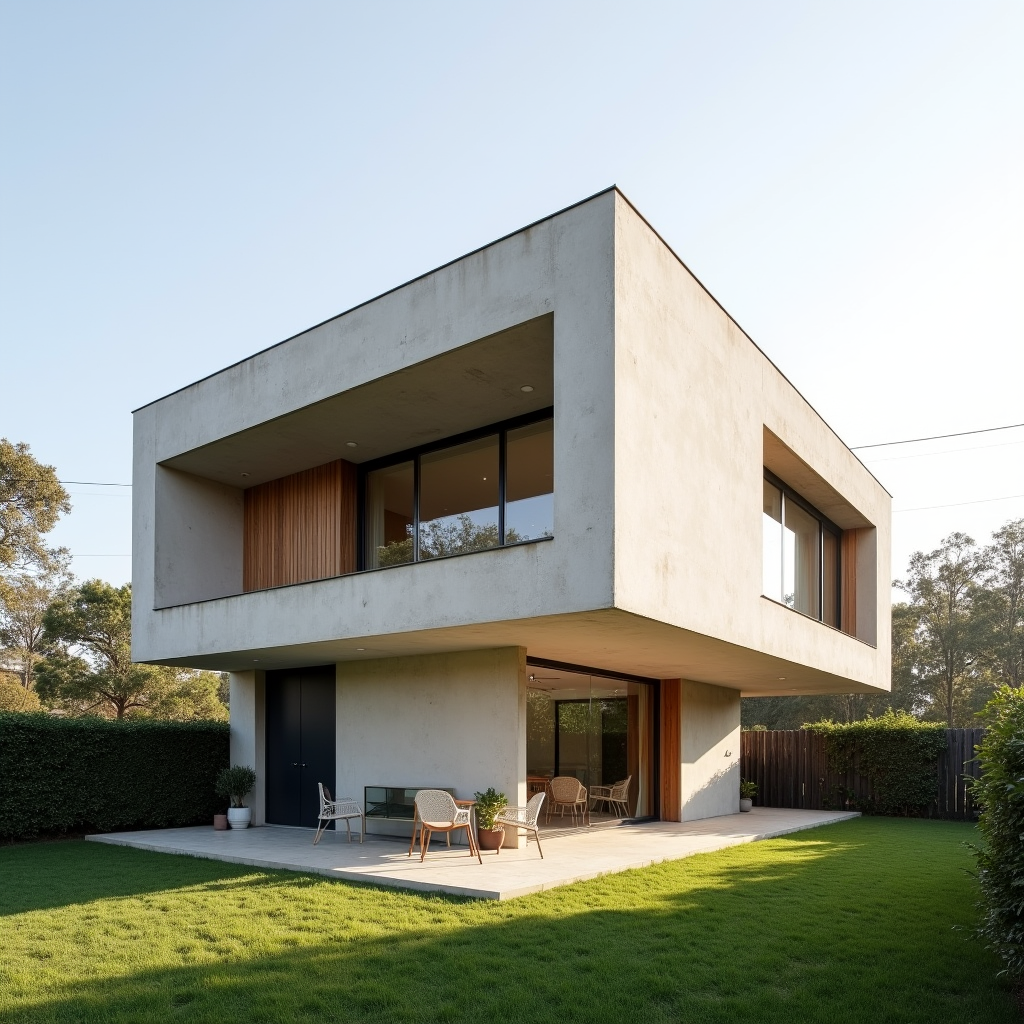
\includegraphics[width=0.12\textwidth]{Images/Results/Architect-A_Fixed-images/2-preliminary_design/Zonder_lora_00061_.png}} &
    \href{https://github.com/matijspeeters/Thesis/blob/main/Images/Results/Architect-A_Fixed-images/2-preliminary_design/Zonder_lora_00069_%20(1).png}{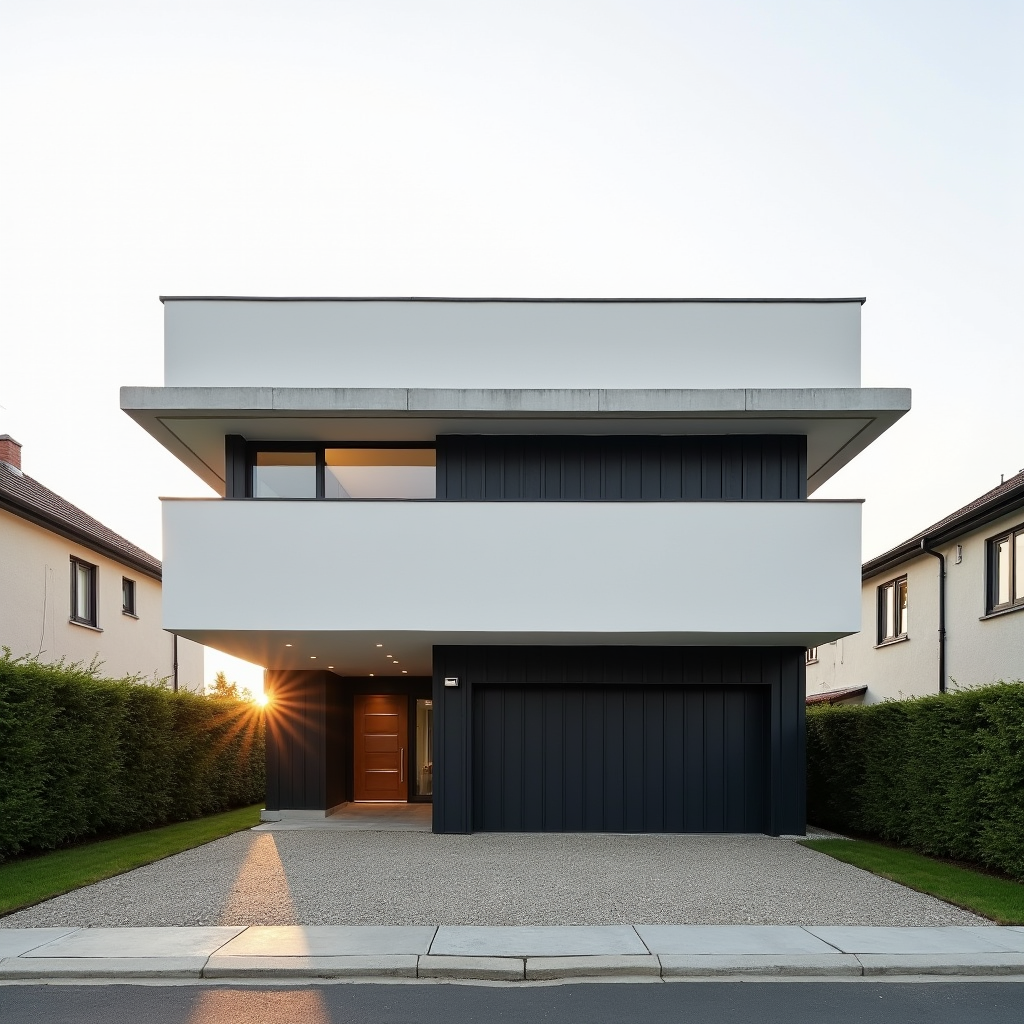
\includegraphics[width=0.12\textwidth]{Images/Results/Architect-A_Fixed-images/2-preliminary_design/Zonder_lora_00069_ (1).png}} &
    \href{https://github.com/matijspeeters/Thesis/blob/main/Images/Results/Architect-A_Fixed-images/2-preliminary_design/Zonder_lora_00080_.png}{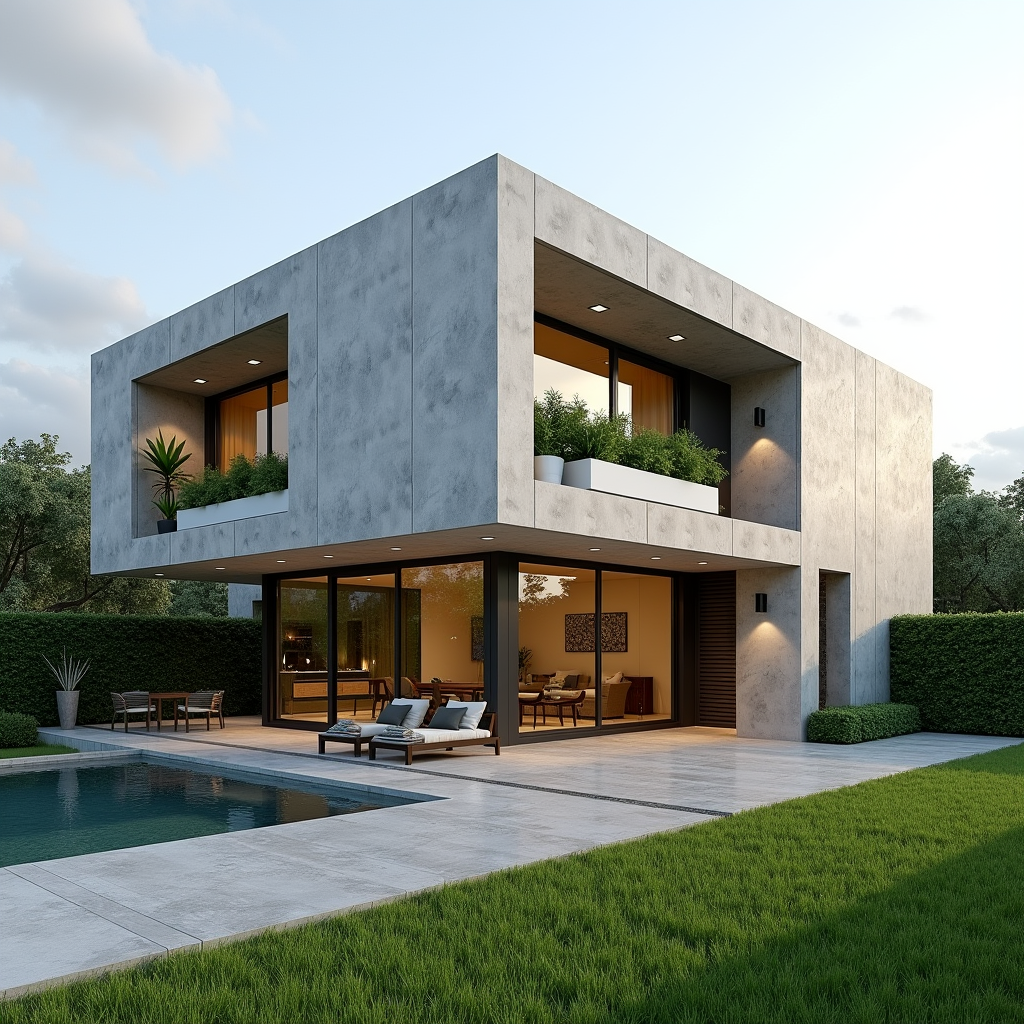
\includegraphics[width=0.12\textwidth]{Images/Results/Architect-A_Fixed-images/2-preliminary_design/Zonder_lora_00080_.png}} &
    \href{https://github.com/matijspeeters/Thesis/blob/main/Images/Results/Architect-A_Fixed-images/2-preliminary_design/Zonder_lora_00089_.png}{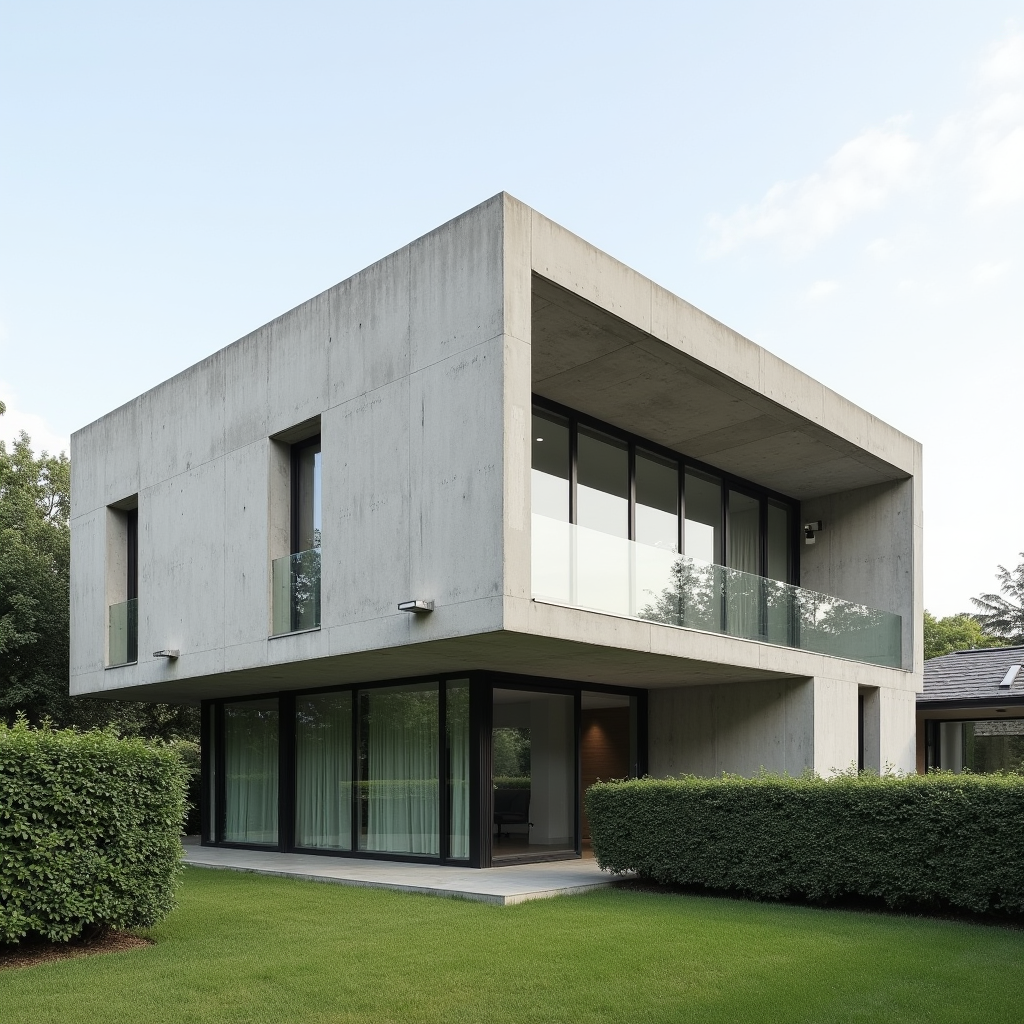
\includegraphics[width=0.12\textwidth]{Images/Results/Architect-A_Fixed-images/2-preliminary_design/Zonder_lora_00089_.png}} &
    \href{https://github.com/matijspeeters/Thesis/blob/main/Images/Results/Architect-A_Fixed-images/2-preliminary_design/Zonder_lora_00091_.png}{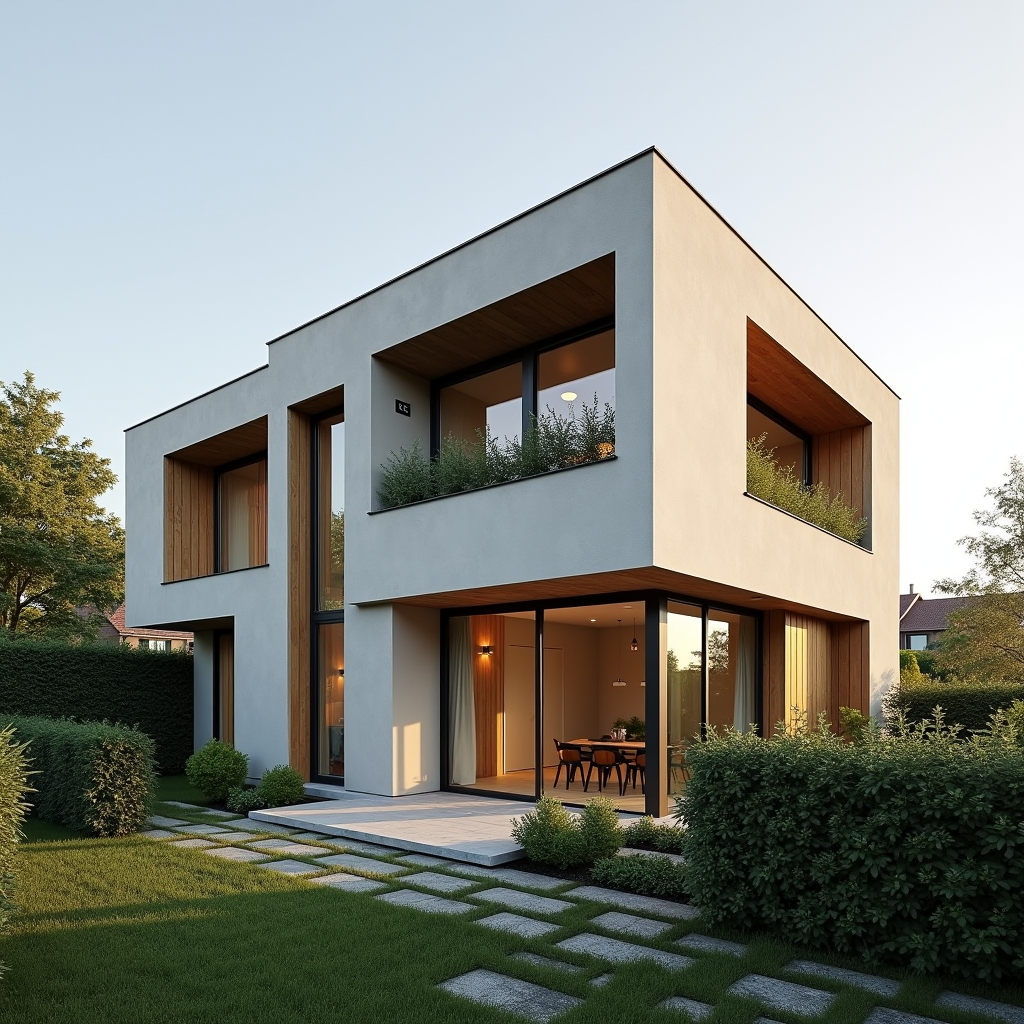
\includegraphics[width=0.12\textwidth]{Images/Results/Architect-A_Fixed-images/2-preliminary_design/Zonder_lora_00091_.png}} &
    \href{https://github.com/matijspeeters/Thesis/blob/main/Images/Results/Architect-A_Fixed-images/2-preliminary_design/Zonder_lora_00095_.png}{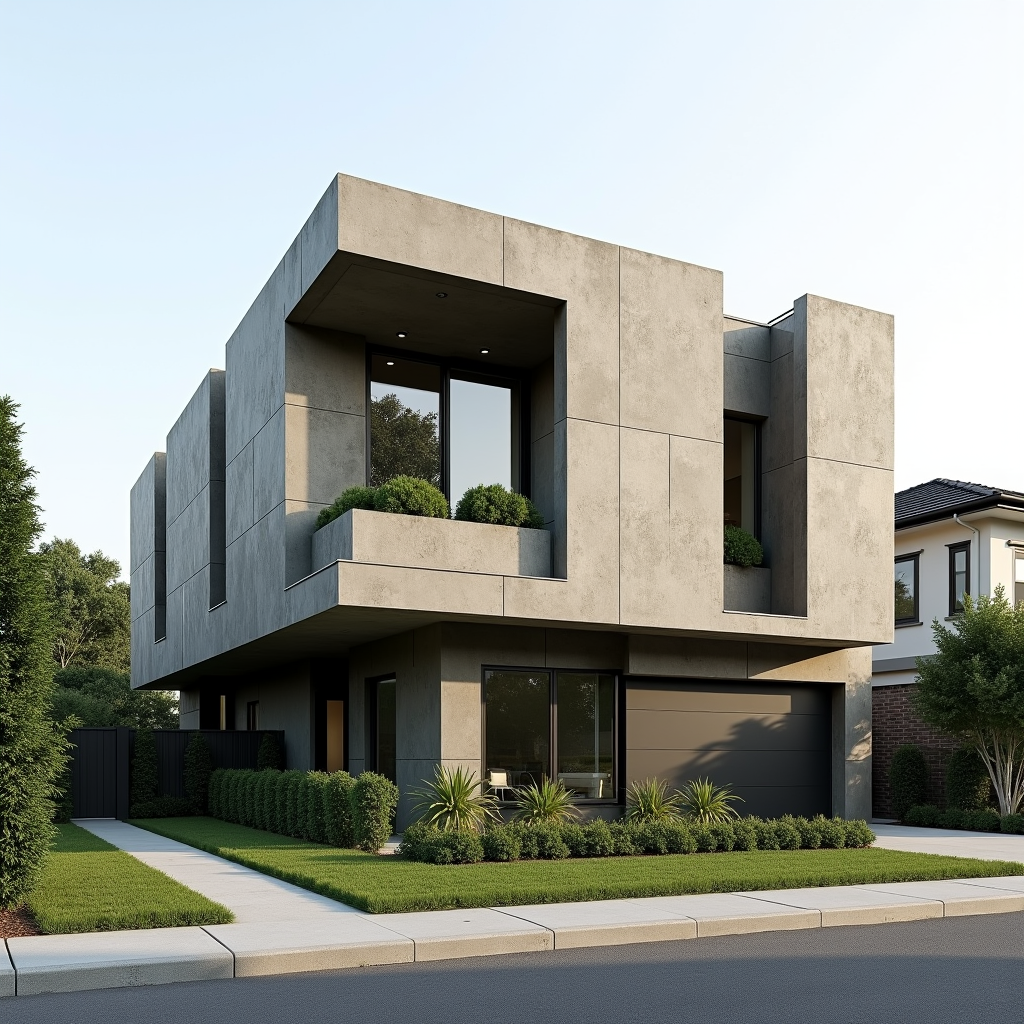
\includegraphics[width=0.12\textwidth]{Images/Results/Architect-A_Fixed-images/2-preliminary_design/Zonder_lora_00095_.png}} \\
  \end{tabular}
  }
  \caption{Starting images in the preliminary design phase of architect A.}
  \label{fig:horizontal-lora-comparison}
\end{figure}
\subsubsection{Selected starting image}
Architect A selected the image in figure \ref{fig:A-preliminary-selected}, which was generated with the \textbf{stampbeton} and \textbf{3D-effect} models. 
\begin{figure}[H]
    \centering
    \href{https://github.com/matijspeeters/Thesis/blob/main/Images/Results/Architect-A_Fixed-images/2-preliminary_design/Met_lora_00080_.png}{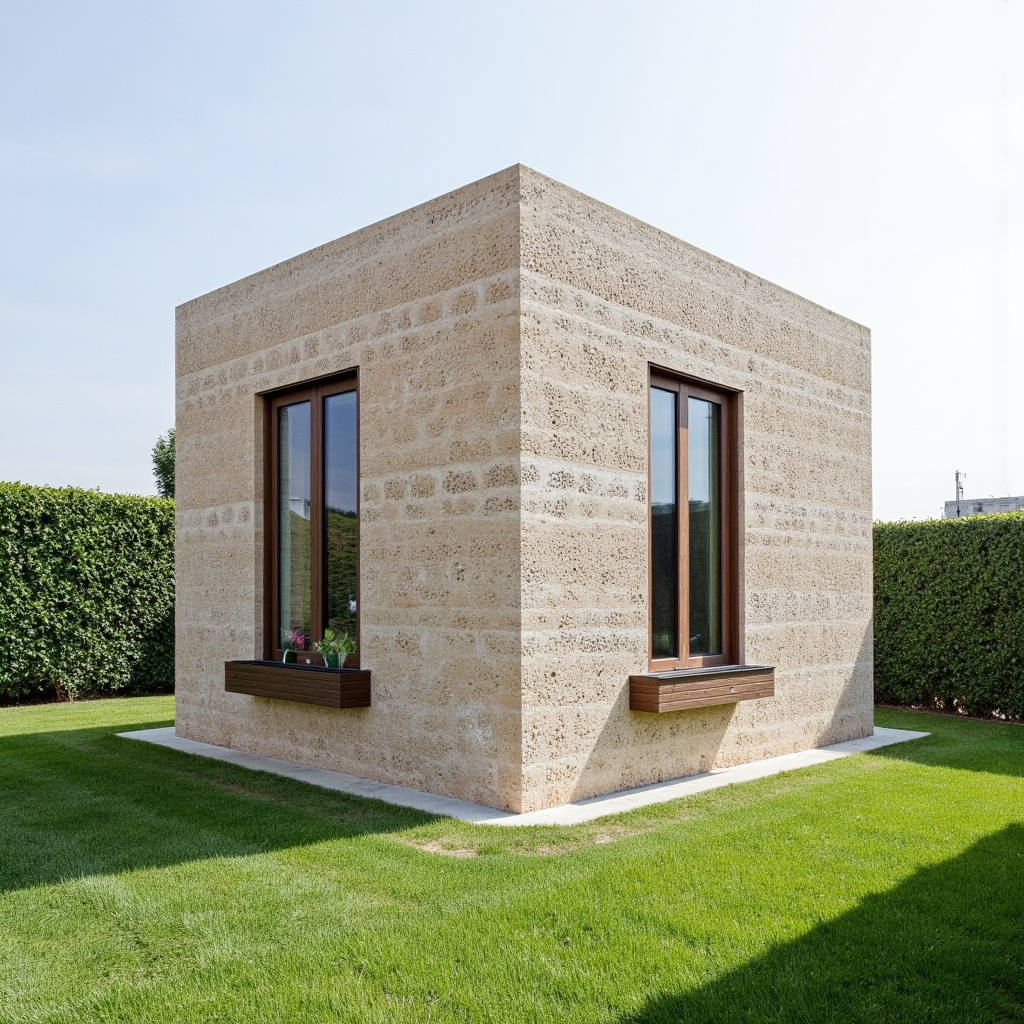
\includegraphics[width=0.3\linewidth]{Images/Results/Architect-A_Fixed-images/2-preliminary_design/Met_lora_00080_.png}}
    \caption{Architect A's selected starting image for the preliminary design phase.}
    \label{fig:A-preliminary-selected}
\end{figure}
\subsubsection{Preferred generated images}
Architect A chose two preferred images among the images generated during this design phase. 
\begin{itemize}
    \item Image 1 was created with LoRAs. Architect A chose this image because
    \item Image 2 was created without LoRAs. Architect A chose this image because 
\end{itemize}
\begin{figure}[H]
    \centering
    \begin{tabular}{cc}
         \href{https://github.com/matijspeeters/Thesis/blob/main/Images/Results/Architect%20A/2.%20Preliminary%20phase/Met_lora_00004_.png}{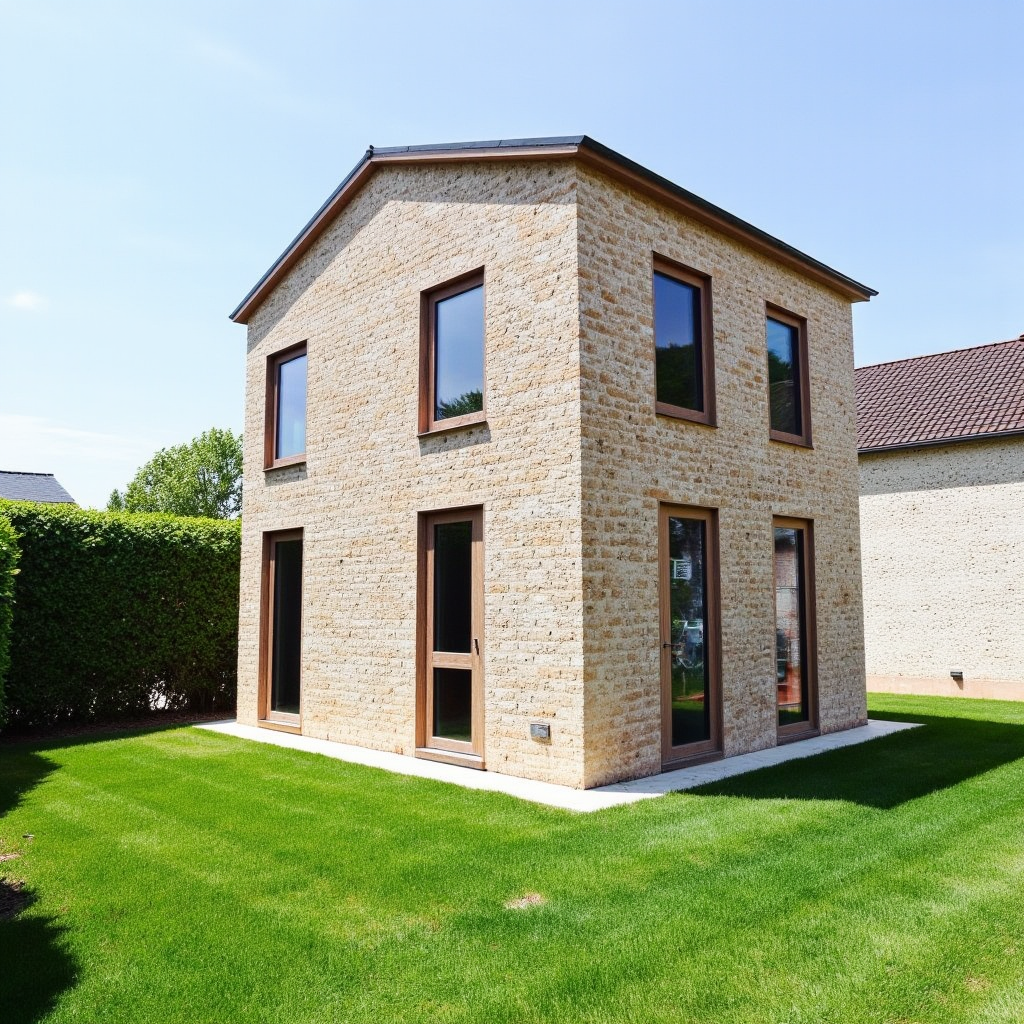
\includegraphics[width=0.3\linewidth]{Images/Results/Architect A/2. Preliminary phase/Met_lora_00004_.png}} & \href{https://github.com/matijspeeters/Thesis/blob/main/Images/Results/Architect%20A/2.%20Preliminary%20phase/Zonder_lora_00146_.png}{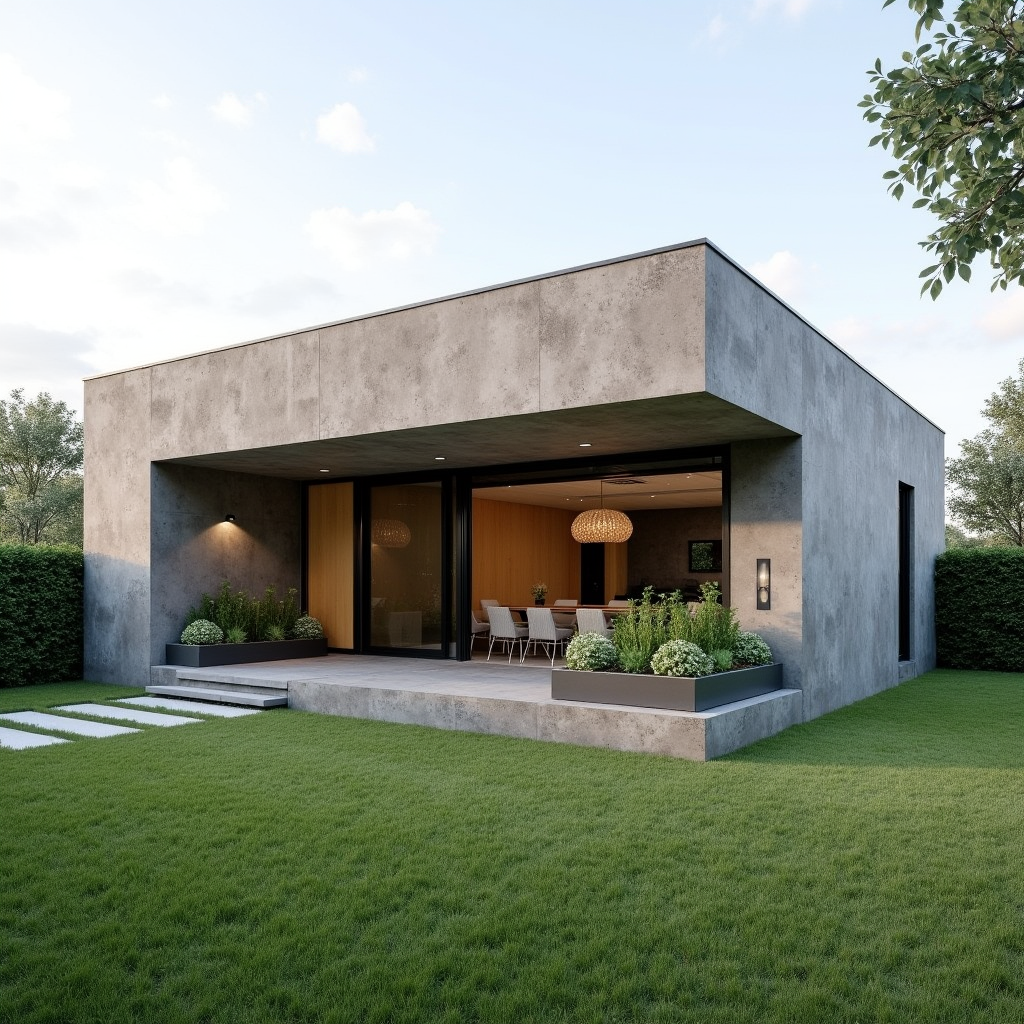
\includegraphics[width=0.3\linewidth]{Images/Results/Architect A/2. Preliminary phase/Zonder_lora_00146_.png}}\\
         \textit{(1)} & \textit{(2)}
    \end{tabular}
    \caption{Architect A's favourite images in the preliminary design phase.}
    \label{fig:A-preliminary-preferred}
\end{figure}

\subsection{Presentation phase}
\subsubsection{Starting images}
\begin{figure}[H]
  \centering
  {\footnotesize
  \renewcommand{\arraystretch}{1.1}
  \setlength{\tabcolsep}{4pt}
  \begin{tabular}{c c c c c c c c}
    & \shortstack{\textbf{Stamp-}\\\textbf{beton}} 
    & \shortstack{\textbf{3D-}\\\textbf{effect}} 
    & \textbf{Geleding} 
    & \shortstack{\textbf{Stampbeton}\\ \textbf{\& 3D-effect}} 
    & \shortstack{\textbf{Stampbeton}\\ \textbf{\& Geleding}} 
    & \shortstack{\textbf{3D-effect} \&\\ \textbf{Geleding}} 
    & \shortstack{\textbf{Stampbeton,}\\\textbf{3D-effect \&}\\\textbf{Geleding}} \\

    \shortstack{\textbf{With}\\\textbf{LoRA}} & 
    \href{https://github.com/matijspeeters/Thesis/blob/main/Images/Results/Architect-A_Fixed-images/3-presentation/Met_lora_00097_.png}{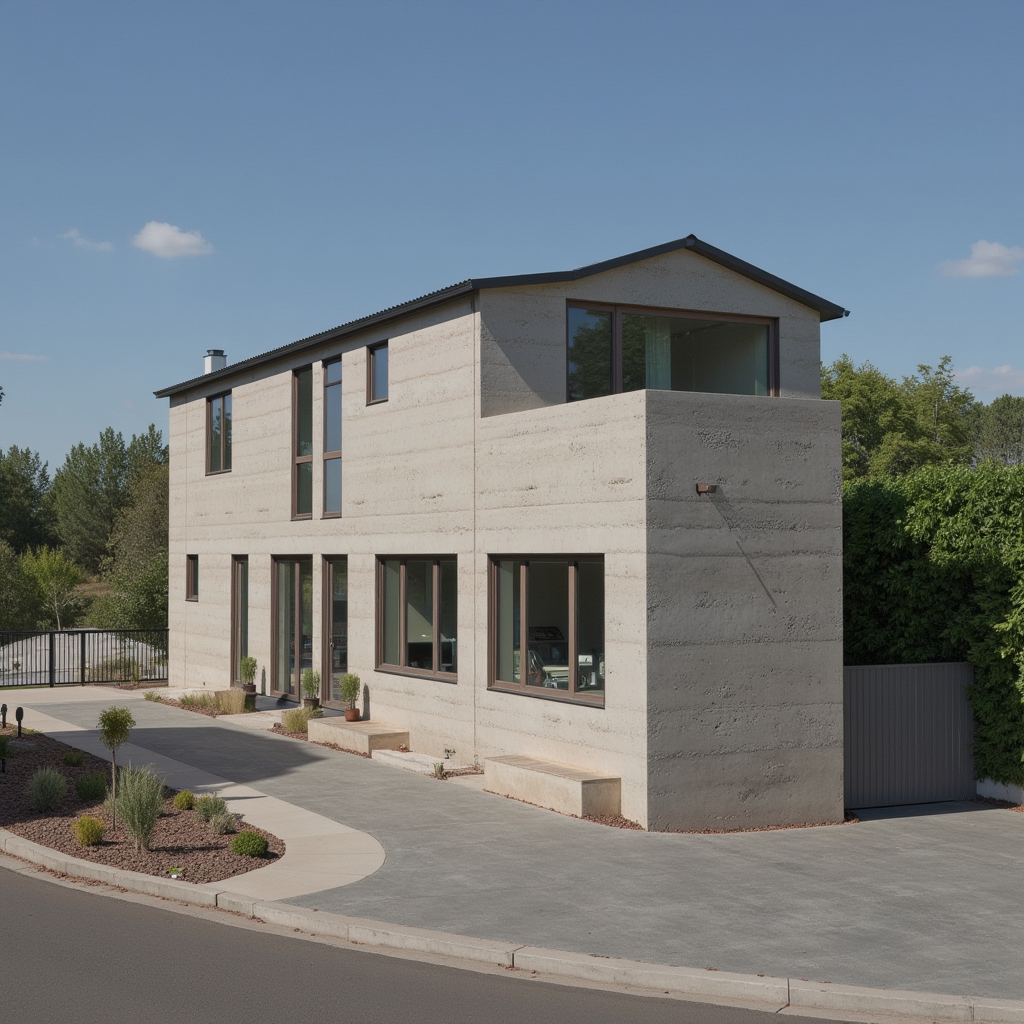
\includegraphics[width=0.12\textwidth]{Images/Results/Architect-A_Fixed-images/3-presentation/Met_lora_00097_.png}} & 
    \href{https://github.com/matijspeeters/Thesis/blob/main/Images/Results/Architect-A_Fixed-images/3-presentation/Met_lora_00100_.png}{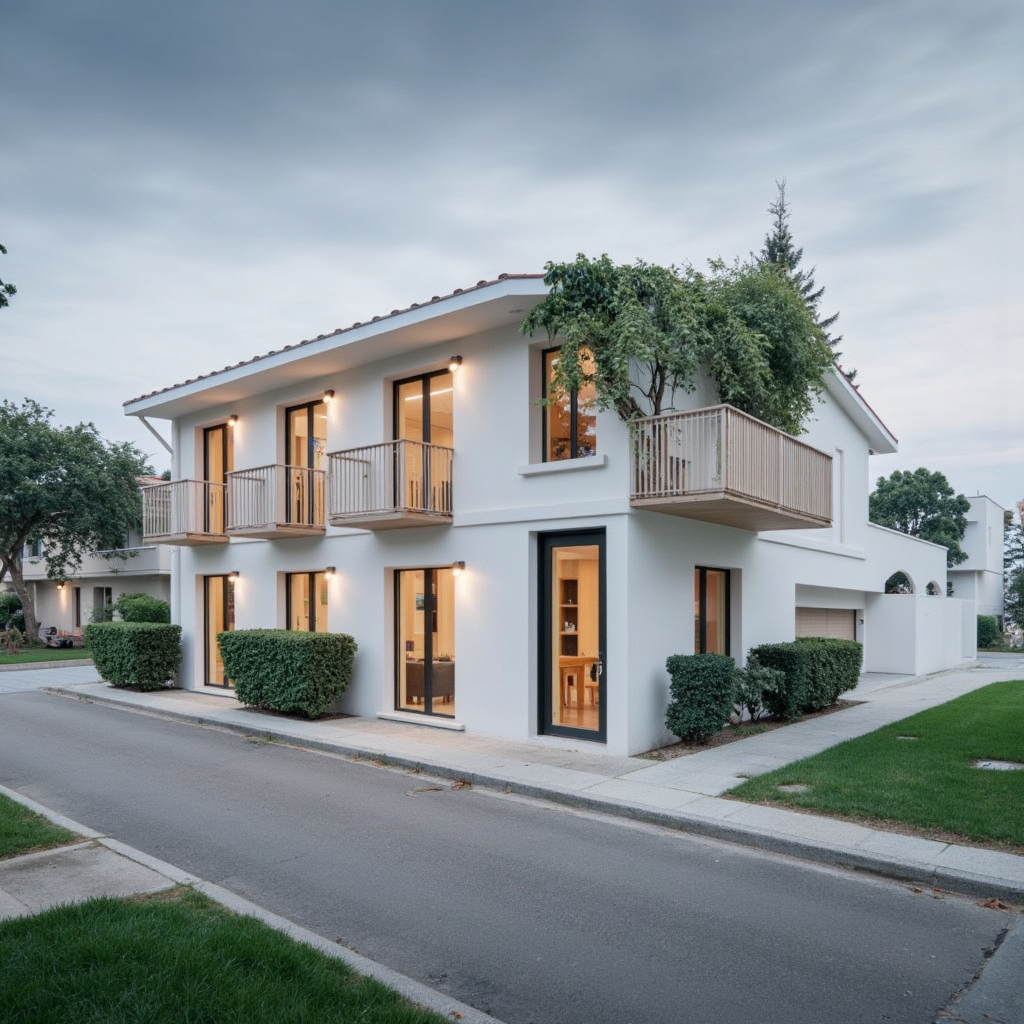
\includegraphics[width=0.12\textwidth]{Images/Results/Architect-A_Fixed-images/3-presentation/Met_lora_00100_.png}} &
    \href{https://github.com/matijspeeters/Thesis/blob/main/Images/Results/Architect-A_Fixed-images/3-presentation/Met_lora_00106_.png}{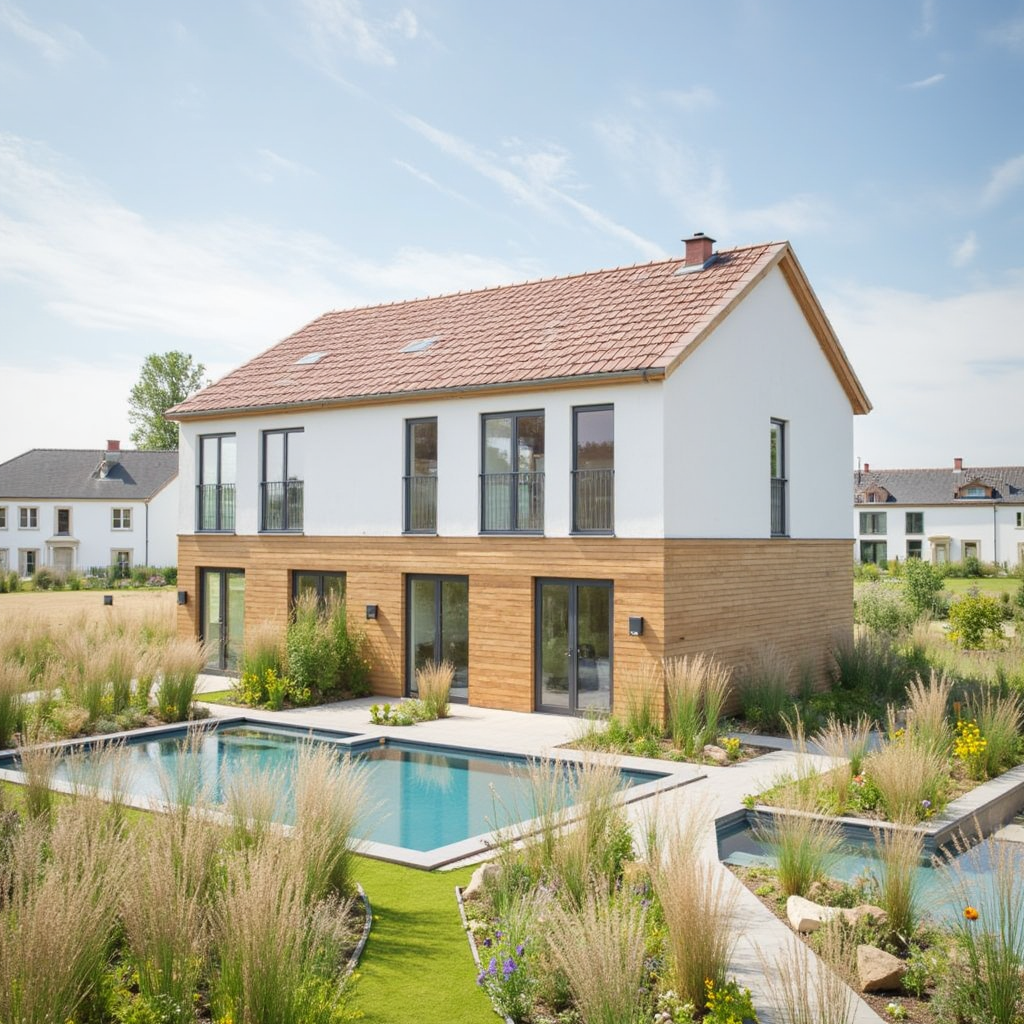
\includegraphics[width=0.12\textwidth]{Images/Results/Architect-A_Fixed-images/3-presentation/Met_lora_00106_.png}} &
    \href{https://github.com/matijspeeters/Thesis/blob/main/Images/Results/Architect-A_Fixed-images/3-presentation/Met_lora_00111_.png}{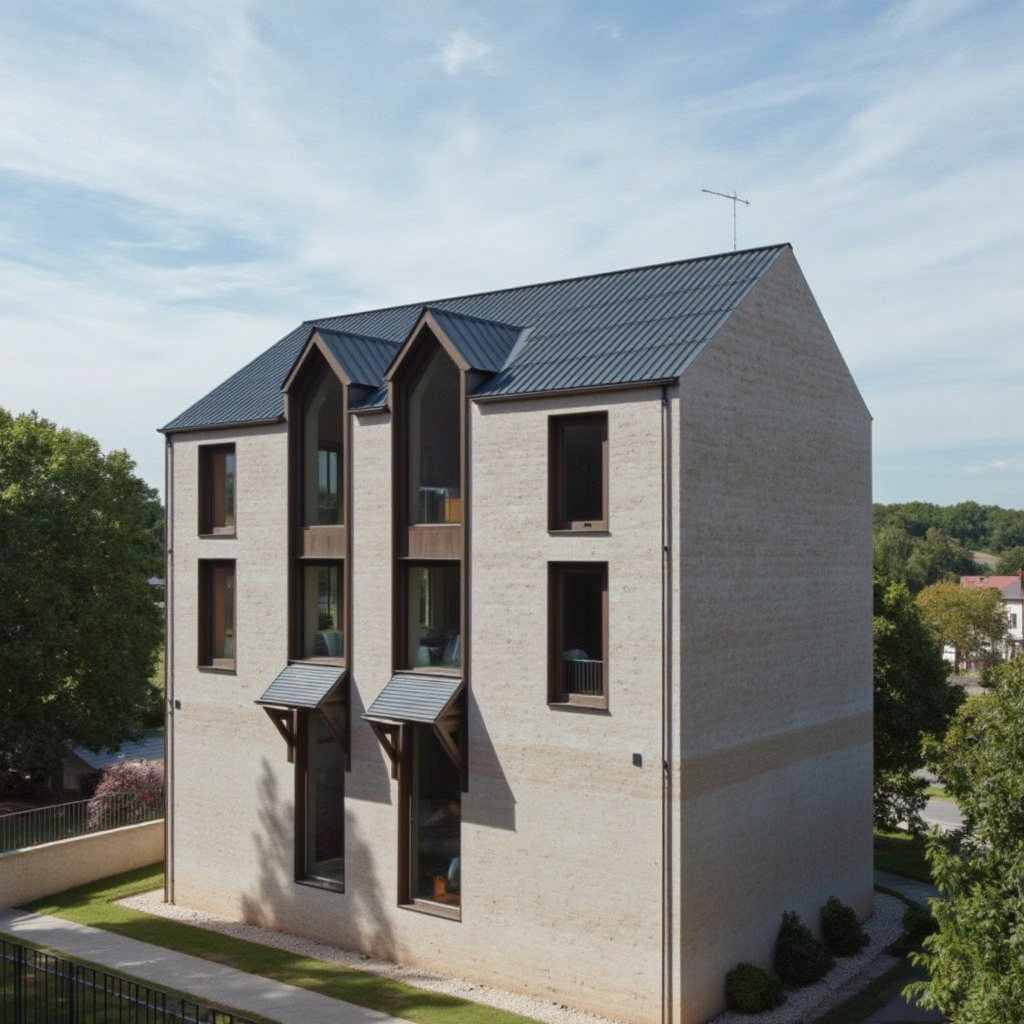
\includegraphics[width=0.12\textwidth]{Images/Results/Architect-A_Fixed-images/3-presentation/Met_lora_00111_.png}} &
    \href{https://github.com/matijspeeters/Thesis/blob/main/Images/Results/Architect-A_Fixed-images/3-presentation/Met_lora_00115_.png}{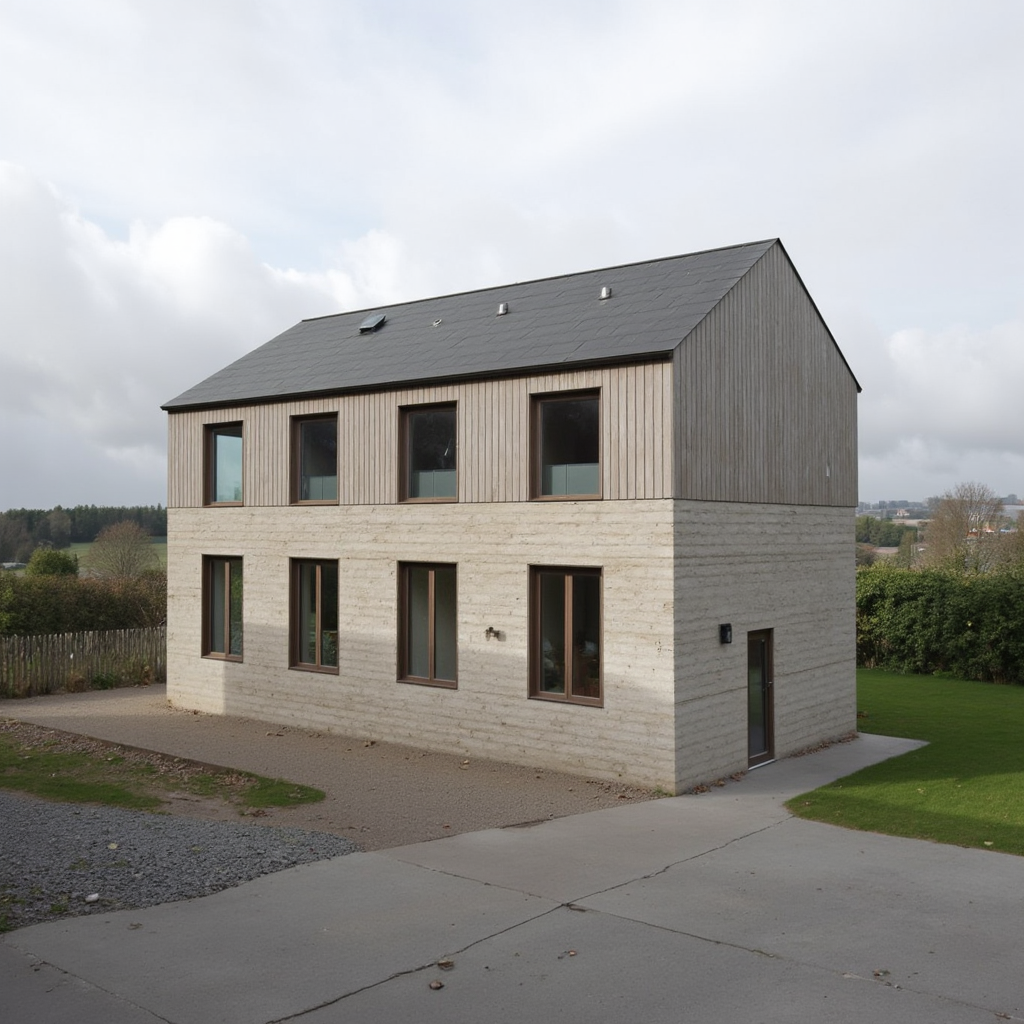
\includegraphics[width=0.12\textwidth]{Images/Results/Architect-A_Fixed-images/3-presentation/Met_lora_00115_.png}} &
    \href{https://github.com/matijspeeters/Thesis/blob/main/Images/Results/Architect-A_Fixed-images/3-presentation/Met_lora_00117_.png}{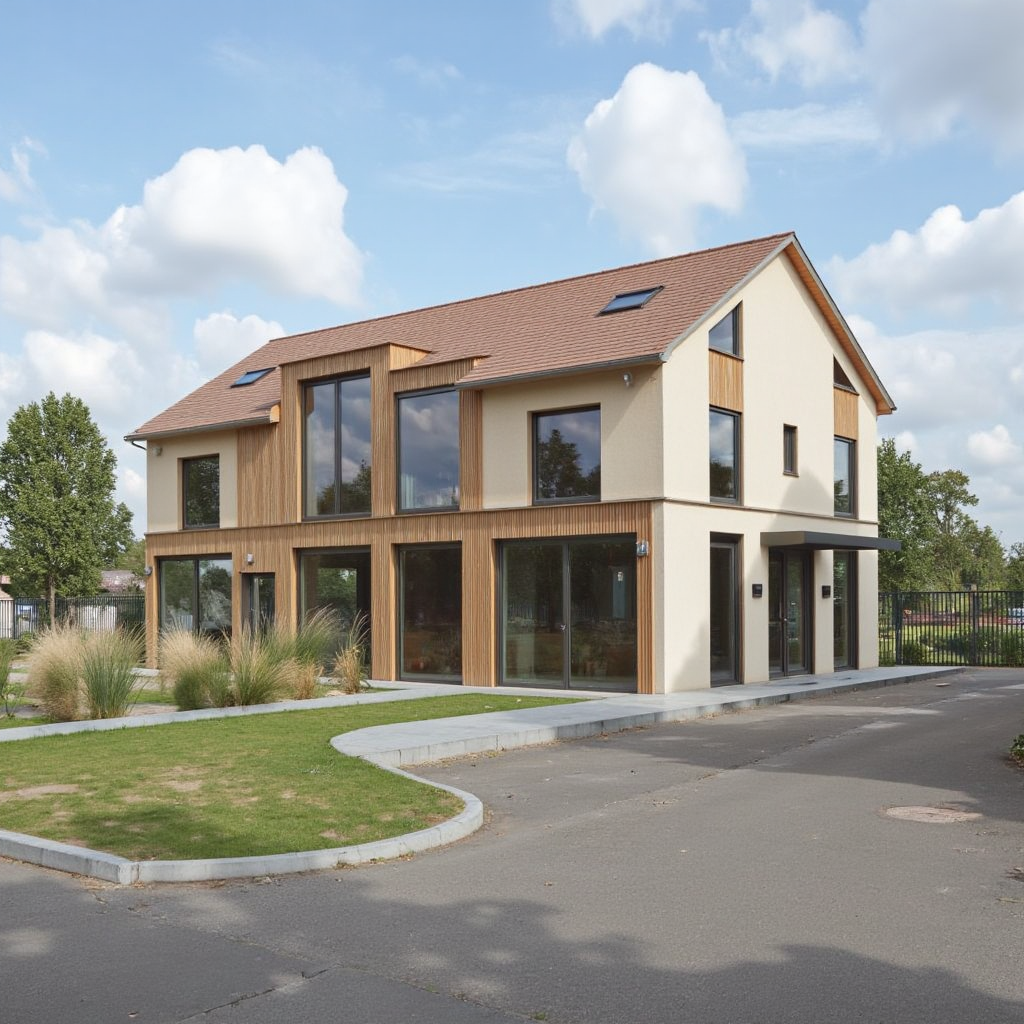
\includegraphics[width=0.12\textwidth]{Images/Results/Architect-A_Fixed-images/3-presentation/Met_lora_00117_.png}} &
    \href{https://github.com/matijspeeters/Thesis/blob/main/Images/Results/Architect-A_Fixed-images/3-presentation/Met_lora_00121_.png}{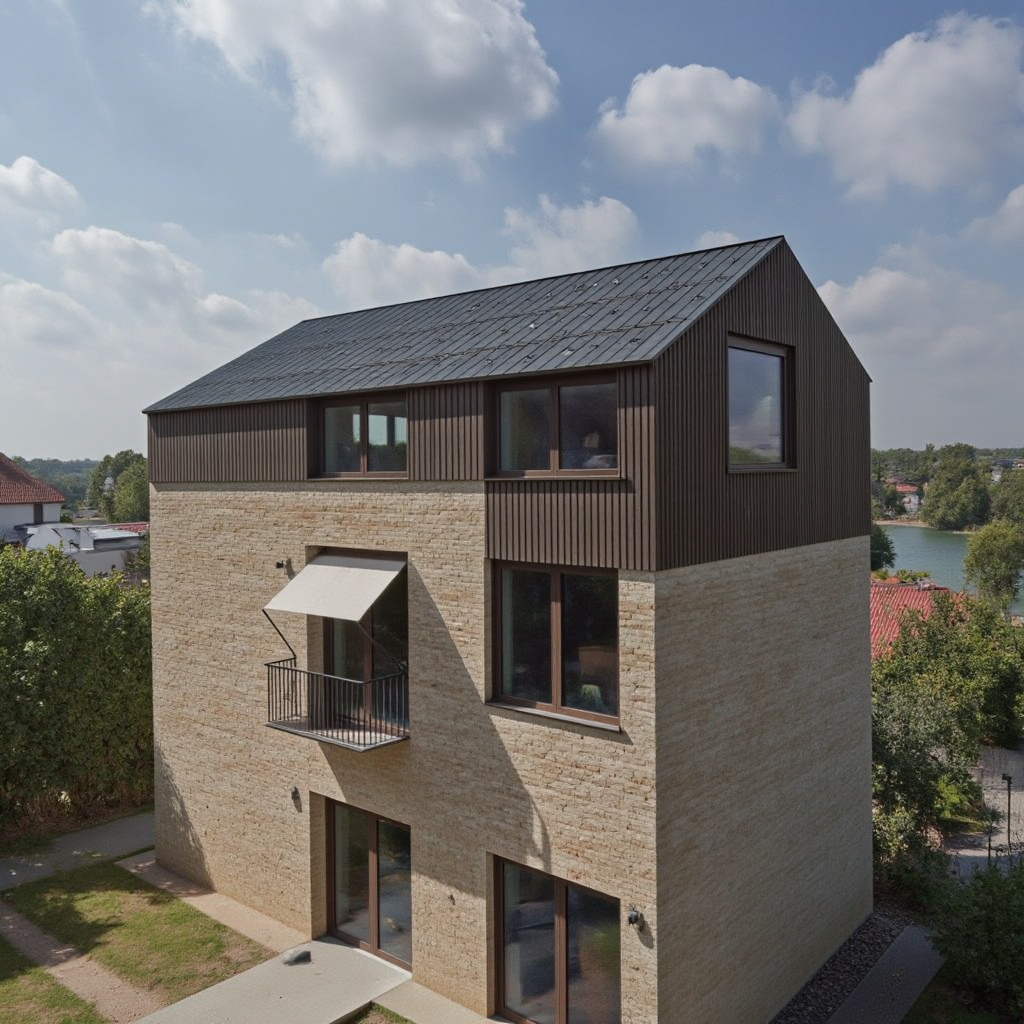
\includegraphics[width=0.12\textwidth]{Images/Results/Architect-A_Fixed-images/3-presentation/Met_lora_00121_.png}} \\

    \shortstack{\textbf{Without}\\\textbf{LoRA}} &
    \href{https://github.com/matijspeeters/Thesis/blob/main/Images/Results/Architect-A_Fixed-images/3-presentation/Zonder_lora_00097_.png}{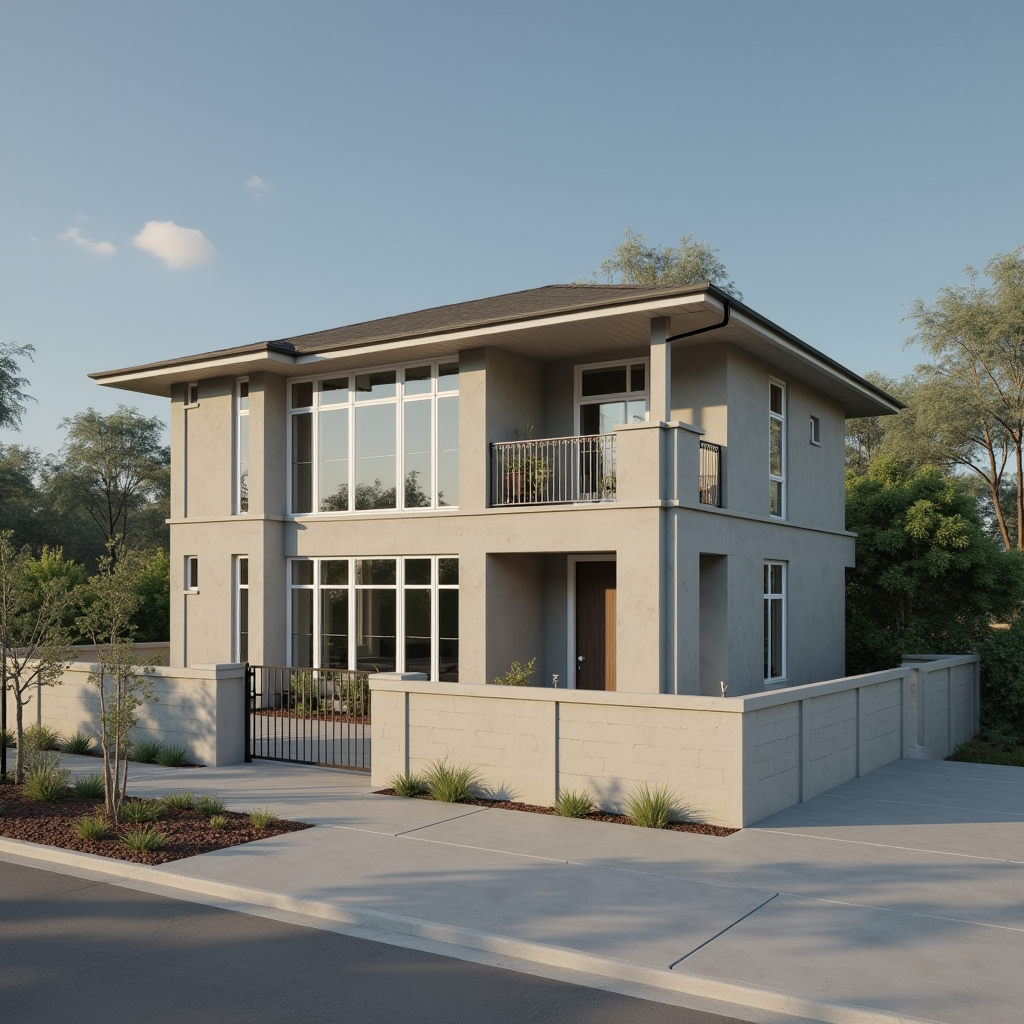
\includegraphics[width=0.12\textwidth]{Images/Results/Architect-A_Fixed-images/3-presentation/Zonder_lora_00097_.png}} &
    \href{https://github.com/matijspeeters/Thesis/blob/main/Images/Results/Architect-A_Fixed-images/3-presentation/Zonder_lora_00100_.png}{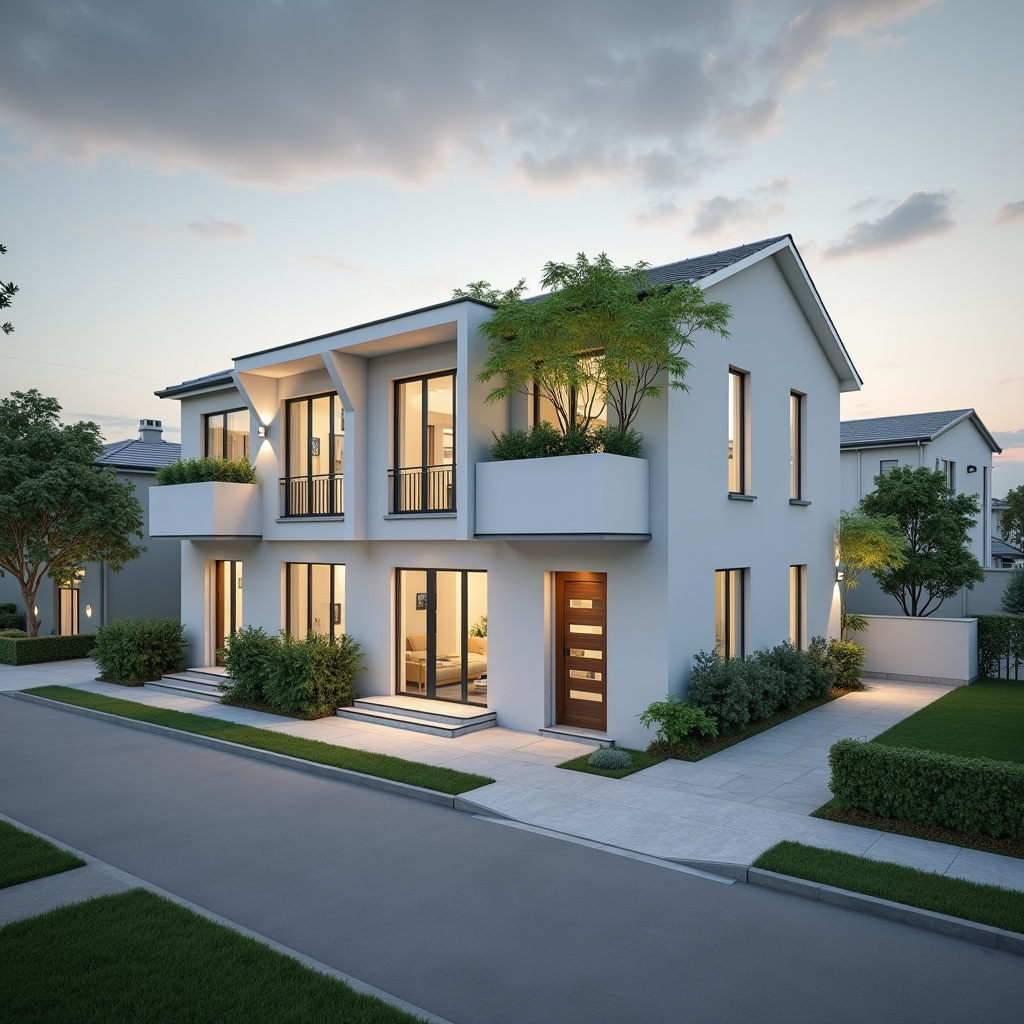
\includegraphics[width=0.12\textwidth]{Images/Results/Architect-A_Fixed-images/3-presentation/Zonder_lora_00100_.png}} &
    \href{https://github.com/matijspeeters/Thesis/blob/main/Images/Results/Architect-A_Fixed-images/3-presentation/Zonder_lora_00106_.png}{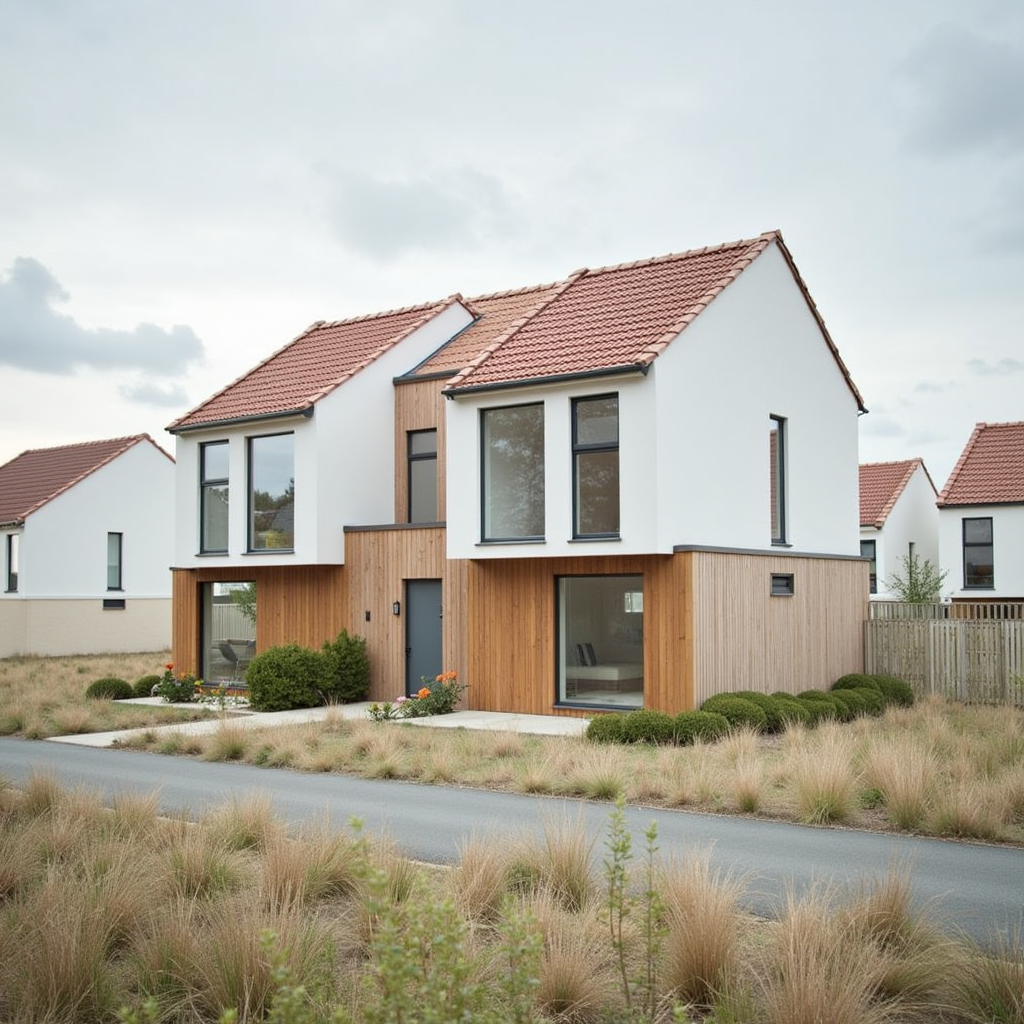
\includegraphics[width=0.12\textwidth]{Images/Results/Architect-A_Fixed-images/3-presentation/Zonder_lora_00106_.png}} &
    \href{https://github.com/matijspeeters/Thesis/blob/main/Images/Results/Architect-A_Fixed-images/3-presentation/Zonder_lora_00111_.png}{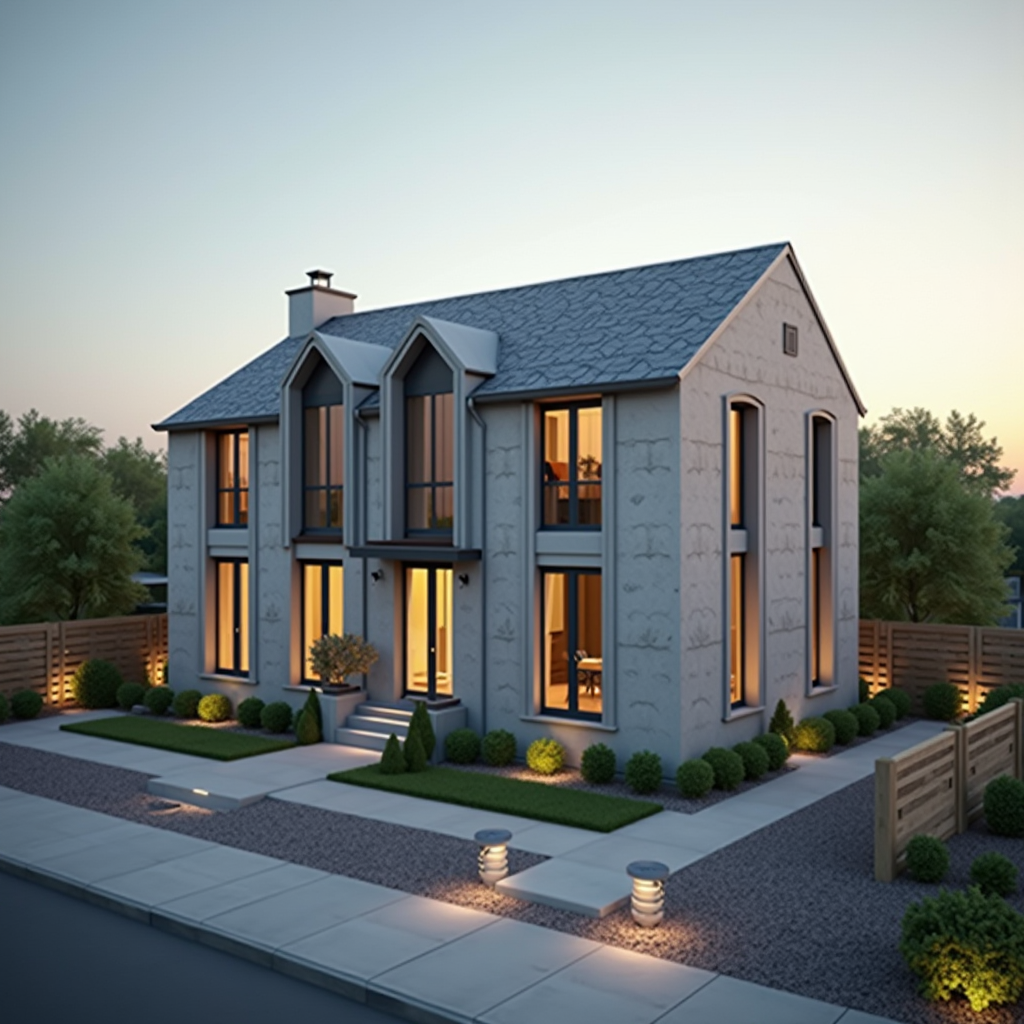
\includegraphics[width=0.12\textwidth]{Images/Results/Architect-A_Fixed-images/3-presentation/Zonder_lora_00111_.png}} &
    \href{https://github.com/matijspeeters/Thesis/blob/main/Images/Results/Architect-A_Fixed-images/3-presentation/Zonder_lora_00115_.png}{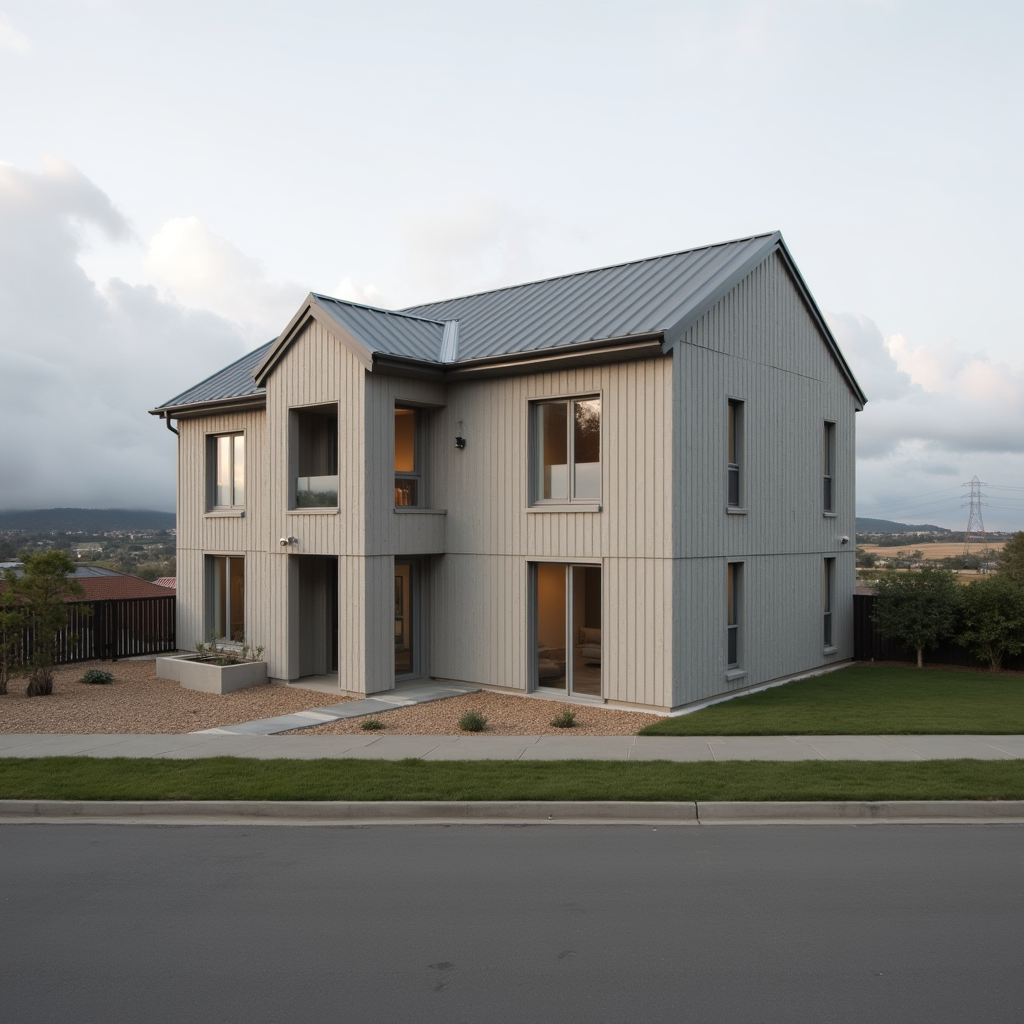
\includegraphics[width=0.12\textwidth]{Images/Results/Architect-A_Fixed-images/3-presentation/Zonder_lora_00115_.png}} &
    \href{https://github.com/matijspeeters/Thesis/blob/main/Images/Results/Architect-A_Fixed-images/3-presentation/Zonder_lora_00117_.png}{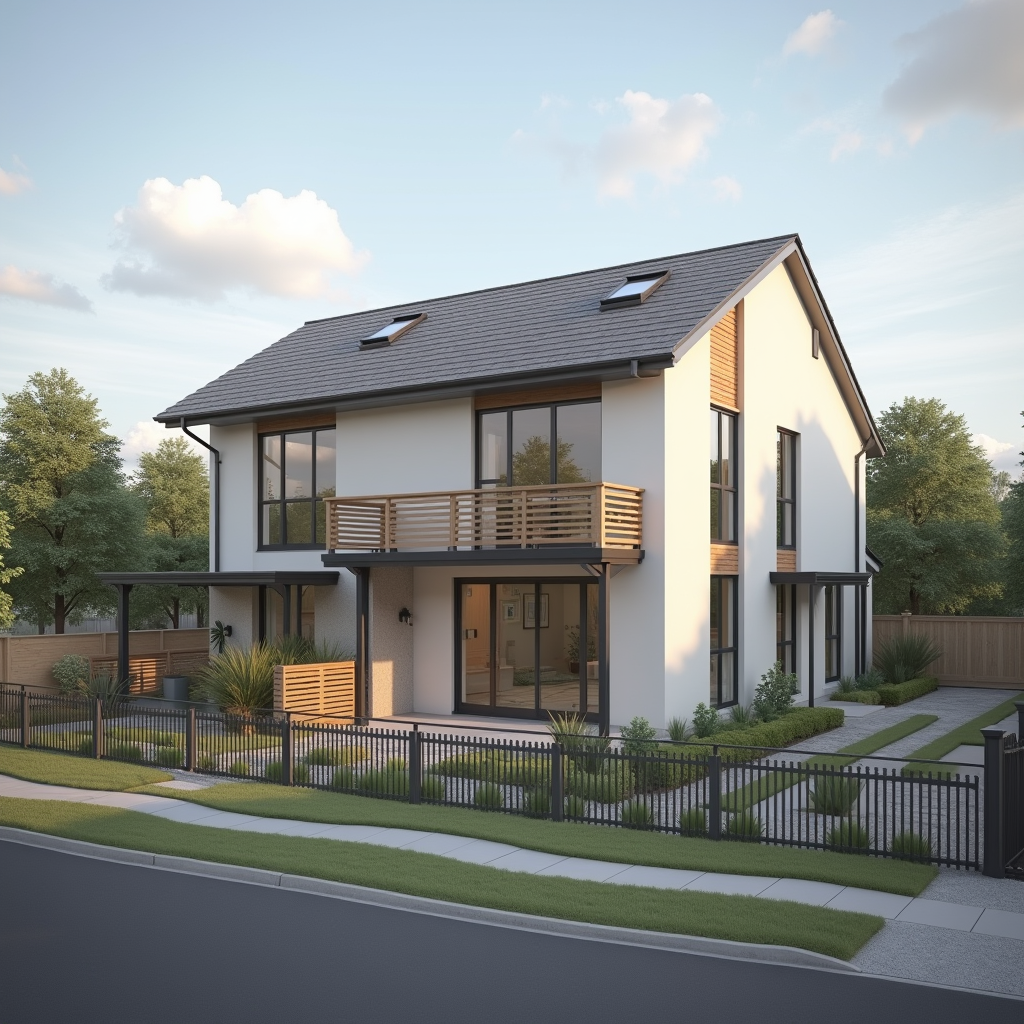
\includegraphics[width=0.12\textwidth]{Images/Results/Architect-A_Fixed-images/3-presentation/Zonder_lora_00117_.png}} &
    \href{https://github.com/matijspeeters/Thesis/blob/main/Images/Results/Architect-A_Fixed-images/3-presentation/Zonder_lora_00121_.png}{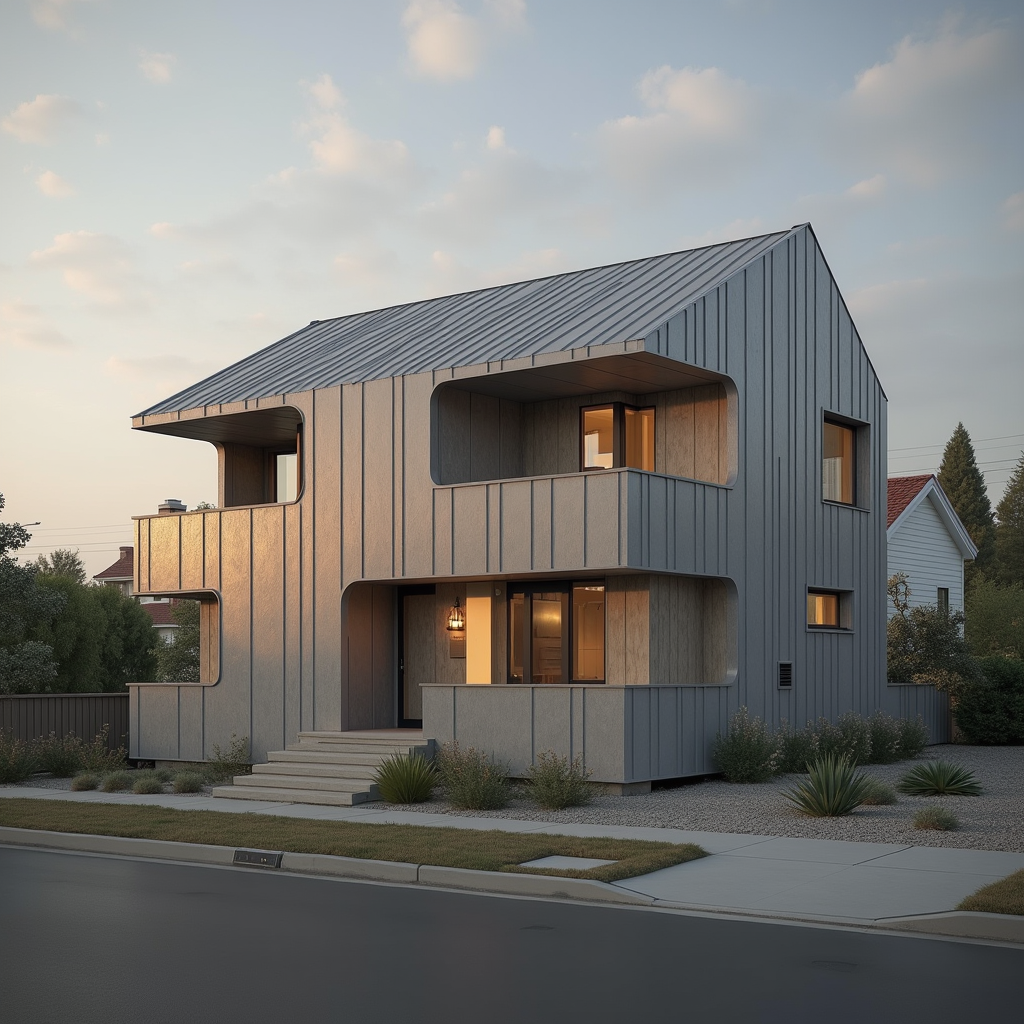
\includegraphics[width=0.12\textwidth]{Images/Results/Architect-A_Fixed-images/3-presentation/Zonder_lora_00121_.png}} \\
  \end{tabular}
  }
  \caption{Starting images in the presentation phase of architect A.}
  \label{fig:horizontal-lora-comparison}
\end{figure}

\subsubsection{Selected starting image}
Architect A selected the image in figure \ref{fig:A-presentation-selected} , which was generated with the stampbeton LoRA. His reasons were the beautiful stamped concrete, and the interaction of the building with the environment. He could 'imagine an interesting location plan'. Additionally, the unusual shape of the roof 'suggests something below it' and 'allows for fun spaces inside'.
\begin{figure}[H]
    \centering
    \href{https://github.com/matijspeeters/Thesis/blob/main/Images/Results/Architect-A_Fixed-images/3-presentation/Met_lora_00097_.png}{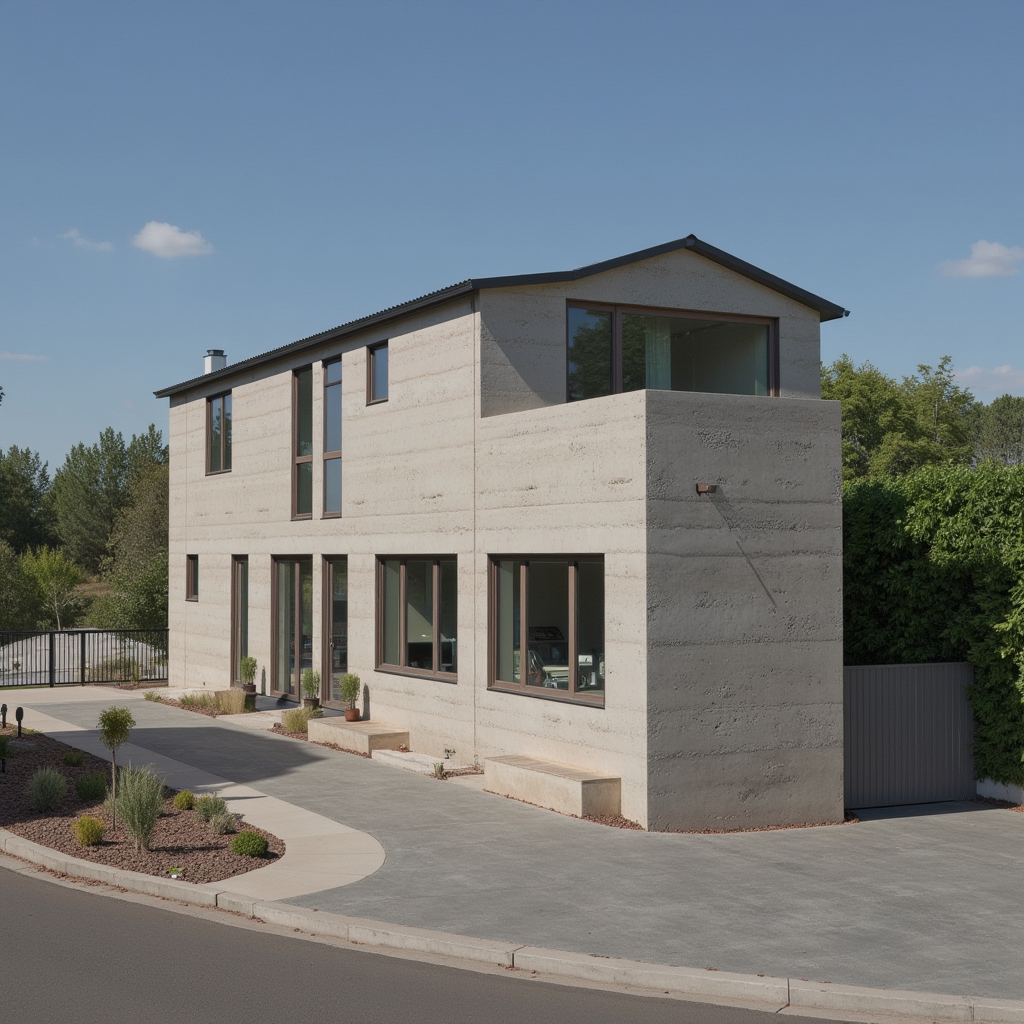
\includegraphics[width=0.3\linewidth]{Images/Results/Architect-A_Fixed-images/3-presentation/Met_lora_00097_.png}}
    \caption{Architect A's selected starting image for the presentation phase.}
    \label{fig:A-presentation-selected}
\end{figure}

\subsubsection{Preferred generated images}
Architect A chose two preferred images among the images generated during this design phase. Both images were created with the \textbf{stampbeton} LoRA. The reasons for image \ref{fig:A-presentation-preferred-A} were the 'layering in the bottom zone, the very simple and balanced volumetry, and the beautiful detailing in the roof'. The reasons for image \ref{fig:A-presentation-preferred-B} were the 'simple volumetry and good stamped concrete'.
\begin{figure}[H]
    \centering
    \begin{subfigure}[b]{0.3\textwidth}
        \centering
        \href{https://github.com/matijspeeters/Thesis/blob/main/Images/Results/Architect%20A/3.%20Presentation%20phase/Met_lora_00002_.png}{\includegraphics[width=\textwidth]{Images/Results/Architect A/3. Presentation phase/Met_lora_00002_.png}}
        \caption{}
        \label{fig:A-presentation-preferred-A}
    \end{subfigure}
    \begin{subfigure}[b]{0.3\textwidth}
        \centering
         \href{https://github.com/matijspeeters/Thesis/blob/main/Images/Results/Architect%20A/3.%20Presentation%20phase/Met_lora_00006_.png}{\includegraphics[width=\textwidth]{Images/Results/Architect A/3. Presentation phase/Met_lora_00006_.png}}
         \caption{}
         \label{fig:A-presentation-preferred-B}
    \end{subfigure}
    \caption{Architect A's preferred images in the presentation phase.}
    \label{fig:A-presentation-preferred}
\end{figure}
\newpage
\subsection{Unstructured phase}
During the unstructured phase, architect A provided several sketches of projects that their office is working on. This section portrays a representative selection of AI-generated images based on these sketches, providing an oversight of how this tool worked based on the architects' sketches.\\
All images were generated by uploading the sketch to the custom GPT, and asking it to write a prompt for that building. Then, this prompt was used in combination with ControlNet, to generate images based on this sketch. Two preprocessors were used for this: canny edge detection and a depth map.\\
For each sketch, only a representative selection of generated images (with and without LoRA) is shown here. All generated images can be found in the appendix of this thesis (chapter \ref{appendix}).
\subsubsection{Sketch 1}
\begin{figure}[H]
    \centering
    \begin{subfigure}[b]{0.3\textwidth}
        \centering
        \includegraphics[width=\textwidth]{Images/Results/Architect-A_unstructured-phase/sketches/sketch_1.png}
        \caption{}
        \label{A-unstructured-1-sketch}
    \end{subfigure}
    \begin{subfigure}[b]{0.3\textwidth}
        \centering 
        \includegraphics[width=\textwidth]{Images/Results/Architect-A_unstructured-phase/sketches/sketch_1_preprocessed.png}
        \caption{}
        \label{A-unstructured-1-sketch-prep}
    \end{subfigure}
    \caption{The first original image provided by architect A (a) and the canny-preprocessed image (b).}
    \label{fig:placeholder}
\end{figure}
To generate images based on this sketch, the architect chose to include all 3 LoRAs: the ground floor of the building should be made out of stampbeton, there is a 3D-effect because of the balconies, and there is an articulation because of the difference between ground floor and the floors above. The researcher wrote a prompt with the custom GPT based on the image, and used the canny edge preprocessor to start generating images with ControlNet.
\begin{figure}[H]
  \centering
  {\footnotesize
  \renewcommand{\arraystretch}{1.1}
  \setlength{\tabcolsep}{4pt}
  \begin{tabular}{c c c c}
    \textbf{With LoRA} &
    \includegraphics[width=0.25\textwidth]{Images/Results/Architect-A_unstructured-phase/generated_images/1/Met_lora_00001_.png} &
    \includegraphics[width=0.25\textwidth]{Images/Results/Architect-A_unstructured-phase/generated_images/1/Met_lora_00002_.png} &
    \includegraphics[width=0.25\textwidth]{Images/Results/Architect-A_unstructured-phase/generated_images/1/Met_lora_00005_.png} \\

    \textbf{Without LoRA} &
    \includegraphics[width=0.25\textwidth]{Images/Results/Architect-A_unstructured-phase/generated_images/1/Zonder_lora_00001_.png} &
    \includegraphics[width=0.25\textwidth]{Images/Results/Architect-A_unstructured-phase/generated_images/1/Zonder_lora_00002_.png} &
    \includegraphics[width=0.25\textwidth]{Images/Results/Architect-A_unstructured-phase/generated_images/1/Zonder_lora_00005_.png} \\
  \end{tabular}
  }
  \caption{Comparison of results with and without LoRA, generated from architect A's first sketch.}
  \label{fig:lora-comparison}
\end{figure}
\subsubsection{Sketch 2}
\begin{figure}[H]
    \centering
    \begin{subfigure}[b]{0.3\textwidth}
        \centering
        \includegraphics[width=\textwidth]{Images/Results/Architect-A_unstructured-phase/sketches/sketch_2.png}
        \caption{}
        \label{A-unstructured-1-sketch}
    \end{subfigure}
    \begin{subfigure}[b]{0.3\textwidth}
        \centering 
        \includegraphics[width=\textwidth]{Images/Results/Architect-A_unstructured-phase/sketches/sketch_2_preprocessed.png}
        \caption{}
        \label{A-unstructured-1-sketch-prep}
    \end{subfigure}
    \caption{The second original image provided by architect A (a) and the canny-preprocessed image (b).}
    \label{fig:placeholder}
\end{figure}
For the second sketch, the architect provided a view of the rear facade of the same building. He chose to only use the 3D-effect LoRA, for the terraces and balconies.\\
Creating the first images, the GPT interpreted the lines on the adjacent houses as a canal, including it in the prompt. The diffusion model, then, overinterpreted this, generating the building next to a canal, as can be seen in figure \ref{fig:lora-comparison-2wide}. After this, the prompt was changed and these images were generated 

\begin{figure}[H]
  \centering
  {\footnotesize
  \renewcommand{\arraystretch}{1.1}
  \setlength{\tabcolsep}{4pt}
  \begin{tabular}{c c c c}
    \textbf{With LoRA} &
    \includegraphics[width=0.25\textwidth]{Images/Results/Architect-A_unstructured-phase/generated_images/2/Met_lora_00008_.png} &
    \includegraphics[width=0.25\textwidth]{Images/Results/Architect-A_unstructured-phase/generated_images/2/Met_lora_00012_.png} &
    \includegraphics[width=0.25\textwidth]{Images/Results/Architect-A_unstructured-phase/generated_images/2/Met_lora_00013_.png} \\

    \textbf{Without LoRA} &
    \includegraphics[width=0.25\textwidth]{Images/Results/Architect-A_unstructured-phase/generated_images/2/Zonder_lora_00008_.png} &
    \includegraphics[width=0.25\textwidth]{Images/Results/Architect-A_unstructured-phase/generated_images/2/Zonder_lora_00012_.png} & \includegraphics[width=0.25\textwidth]{Images/Results/Architect-A_unstructured-phase/generated_images/2/Zonder_lora_00013_.png} \\
  \end{tabular}
  }
  \caption{Comparison of results with and without LoRA, generated from architect A's second sketch.}
  \label{fig:lora-comparison-2wide}
\end{figure}
After this, the researcher generated images with a depth map preprocessor (figure \ref{fig:depth map}).
\begin{figure}[H]
    \centering
    \includegraphics[width=0.3\linewidth]{Images/Results/Architect-A_unstructured-phase/sketches/sketch_2_preprocessed_2.png}
    \caption{The depth map based on architect A's second sketch.}
    \label{fig:depth map}
\end{figure}

\begin{figure}[H]
  \centering
  {\footnotesize
  \renewcommand{\arraystretch}{1.1}
  \setlength{\tabcolsep}{4pt}
  \begin{tabular}{c c c c}
    \textbf{With LoRA} &
    \includegraphics[width=0.25\textwidth]{Images/Results/Architect-A_unstructured-phase/generated_images/2/Met_lora_00015_.png} &
    \includegraphics[width=0.25\textwidth]{Images/Results/Architect-A_unstructured-phase/generated_images/2/Met_lora_00016_.png} &
    \includegraphics[width=0.25\textwidth]{Images/Results/Architect-A_unstructured-phase/generated_images/2/Met_lora_00017_.png} \\

    \textbf{Without LoRA} &
    \includegraphics[width=0.25\textwidth]{Images/Results/Architect-A_unstructured-phase/generated_images/2/Zonder_lora_00015_.png} &
    \includegraphics[width=0.25\textwidth]{Images/Results/Architect-A_unstructured-phase/generated_images/2/Zonder_lora_00016_.png} & \includegraphics[width=0.25\textwidth]{Images/Results/Architect-A_unstructured-phase/generated_images/2/Zonder_lora_00017_.png} \\
  \end{tabular}
  }
  \caption{Comparison of results with and without LoRA, generated from architect A's second sketch using a depth map preprocessor.}
  \label{fig:lora-comparison-2wide}
\end{figure}
\subsubsection{Sketch 3}
\begin{figure}[H]
    \centering
    \begin{subfigure}[b]{0.3\textwidth}
        \centering
        \includegraphics[width=\textwidth]{Images/Results/Architect-A_unstructured-phase/sketches/sketch_3.jpeg}
        \caption{}
        \label{A-unstructured-3-sketch}
    \end{subfigure}
    \begin{subfigure}[b]{0.3\textwidth}
        \centering 
        \includegraphics[width=\textwidth]{Images/Results/Architect-A_unstructured-phase/sketches/sketch_3_preprocessed.jpg}
        \caption{}
        \label{A-unstructured-3-sketch-prep}
    \end{subfigure}
    \caption{The third original image provided by architect A (a) and the canny-preprocessed image (b).}
    \label{fig:placeholder}
\end{figure}
For the third sketch, the architect provided a clearer sketch for a new project. For this image, the architect chose to use the geleding LoRA, and prompted to make a material distinction between the ground floor and the first floor.
\begin{figure}[H]
  \centering
  {\footnotesize
  \renewcommand{\arraystretch}{1.1}
  \setlength{\tabcolsep}{4pt}
  \begin{tabular}{c c c c}
    \textbf{With LoRA} & \includegraphics[width=0.25\textwidth]{Images/Results/Architect-A_unstructured-phase/generated_images/3/Met_lora_00019_.png} & \includegraphics[width=0.25\textwidth]{Images/Results/Architect-A_unstructured-phase/generated_images/3/Met_lora_00023_.png} & \includegraphics[width=0.25\textwidth]{Images/Results/Architect-A_unstructured-phase/generated_images/3/Met_lora_00026_.png} \\
    \textbf{Without LoRA} & \includegraphics[width=0.25\textwidth]{Images/Results/Architect-A_unstructured-phase/generated_images/3/Zonder_lora_00019_.png} & \includegraphics[width=0.25\textwidth]{Images/Results/Architect-A_unstructured-phase/generated_images/3/Zonder_lora_00023_.png} & \includegraphics[width=0.25\textwidth]{Images/Results/Architect-A_unstructured-phase/generated_images/3/Zonder_lora_00026_.png} \\
  \end{tabular}
  }
  \caption{Comparison of results with and without LoRA, generated from architect A's third sketch.}
  \label{fig:A-generatedimgs-sketch3}
\end{figure}

\section{Architect B} \label{sec:results-B}
\subsection{Sketch design phase}
\subsubsection{Starting images}
\begin{figure}[H]
  \centering
  {\footnotesize
  \renewcommand{\arraystretch}{1.1}
  \setlength{\tabcolsep}{4pt}
  \begin{tabular}{c c c c c c c c}
    & \textbf{Ghoek} & \textbf{Modulariteit} & \shortstack{\textbf{Plint-}\\\textbf{werking}}
    & \shortstack{\textbf{Ghoek \&}\\ \textbf{modulari-}\\\textbf{teit}} 
    & \shortstack{\textbf{Ghoek \&}\\ \textbf{Plintwerking}} 
    & \shortstack{\textbf{Modulariteit} \\ \textbf{ \& Plint-}\\\textbf{werking}} 
    & \shortstack{\textbf{Ghoek,}\\\textbf{Modulari-}\\\textbf{teit \&}\\\textbf{PLintwerking}} \\

    \shortstack{\textbf{With}\\\textbf{LoRA}} & 
    \href{https://github.com/matijspeeters/Thesis/blob/main/Images/Results/Architect-B_Fixed-images/1-sketch_design/Met_lora_00004_.png}{\includegraphics[width=0.12\textwidth]{Images/Results/Architect-B_Fixed-images/1-sketch_design/Met_lora_00004_.png}} & 
    \href{https://github.com/matijspeeters/Thesis/blob/main/Images/Results/Architect-B_Fixed-images/1-sketch_design/Met_lora_00007_.png}{\includegraphics[width=0.12\textwidth]{Images/Results/Architect-B_Fixed-images/1-sketch_design/Met_lora_00007_.png}} &
    \href{https://github.com/matijspeeters/Thesis/blob/main/Images/Results/Architect-B_Fixed-images/1-sketch_design/Met_lora_00010_.png}{\includegraphics[width=0.12\textwidth]{Images/Results/Architect-B_Fixed-images/1-sketch_design/Met_lora_00010_.png}} &
    \href{https://github.com/matijspeeters/Thesis/blob/main/Images/Results/Architect-B_Fixed-images/1-sketch_design/Met_lora_00017_.png}{\includegraphics[width=0.12\textwidth]{Images/Results/Architect-B_Fixed-images/1-sketch_design/Met_lora_00017_.png}} &
    \href{https://github.com/matijspeeters/Thesis/blob/main/Images/Results/Architect-B_Fixed-images/1-sketch_design/Met_lora_00021_.png}{\includegraphics[width=0.12\textwidth]{Images/Results/Architect-B_Fixed-images/1-sketch_design/Met_lora_00021_.png}} &
    \href{https://github.com/matijspeeters/Thesis/blob/main/Images/Results/Architect-B_Fixed-images/1-sketch_design/Met_lora_00024_.png}{\includegraphics[width=0.12\textwidth]{Images/Results/Architect-B_Fixed-images/1-sketch_design/Met_lora_00024_.png}} &
    \href{https://github.com/matijspeeters/Thesis/blob/main/Images/Results/Architect-B_Fixed-images/1-sketch_design/Met_lora_00026_.png}{\includegraphics[width=0.12\textwidth]{Images/Results/Architect-B_Fixed-images/1-sketch_design/Met_lora_00026_.png}} \\

    \shortstack{\textbf{Without}\\\textbf{LoRA}} &
    \href{https://github.com/matijspeeters/Thesis/blob/main/Images/Results/Architect-B_Fixed-images/1-sketch_design/Zonder_lora_00004_.png}{\includegraphics[width=0.12\textwidth]{Images/Results/Architect-B_Fixed-images/1-sketch_design/Zonder_lora_00004_.png}} &
    \href{https://github.com/matijspeeters/Thesis/blob/main/Images/Results/Architect-B_Fixed-images/1-sketch_design/Zonder_lora_00007_.png}{\includegraphics[width=0.12\textwidth]{Images/Results/Architect-B_Fixed-images/1-sketch_design/Zonder_lora_00007_.png}} &
    \href{https://github.com/matijspeeters/Thesis/blob/main/Images/Results/Architect-B_Fixed-images/1-sketch_design/Zonder_lora_00010_.png}{\includegraphics[width=0.12\textwidth]{Images/Results/Architect-B_Fixed-images/1-sketch_design/Zonder_lora_00010_.png}} &
    \href{https://github.com/matijspeeters/Thesis/blob/main/Images/Results/Architect-B_Fixed-images/1-sketch_design/Zonder_lora_00017_.png}{\includegraphics[width=0.12\textwidth]{Images/Results/Architect-B_Fixed-images/1-sketch_design/Zonder_lora_00017_.png}} &
    \href{https://github.com/matijspeeters/Thesis/blob/main/Images/Results/Architect-B_Fixed-images/1-sketch_design/Zonder_lora_00021_.png}{\includegraphics[width=0.12\textwidth]{Images/Results/Architect-B_Fixed-images/1-sketch_design/Zonder_lora_00021_.png}} &
    \href{https://github.com/matijspeeters/Thesis/blob/main/Images/Results/Architect-B_Fixed-images/1-sketch_design/Zonder_lora_00024_.png}{\includegraphics[width=0.12\textwidth]{Images/Results/Architect-B_Fixed-images/1-sketch_design/Zonder_lora_00024_.png}} &
    \href{https://github.com/matijspeeters/Thesis/blob/main/Images/Results/Architect-B_Fixed-images/1-sketch_design/Zonder_lora_00026_.png}{\includegraphics[width=0.12\textwidth]{Images/Results/Architect-B_Fixed-images/1-sketch_design/Zonder_lora_00026_.png}} \\
  \end{tabular}
  }
  \caption{Starting images in the sketch design phase of architect B.}
  \label{fig:horizontal-lora-comparison}
\end{figure}

\subsubsection{Selected starting image}
Architect B at first selected the image in figure \ref{fig:B-sketch-selected-a}, which was generated without any LoRAs. When told which images were trained and which were not, the architect changed his choice to the image in figure \ref{fig:B-sketch-selected-b}, which was generated with all LoRAs; Ghoek, Modulariteit and Plintwerking.
\begin{figure}[H]
    \centering
    \begin{subfigure}[b]{0.3\textwidth}
        \centering
        \href{https://github.com/matijspeeters/Thesis/blob/main/Images/Results/Architect-B_Fixed-images/1-sketch_design/Zonder_lora_00007_.png}{\includegraphics[width=\textwidth]{Images/Results/Architect-B_Fixed-images/1-sketch_design/Zonder_lora_00007_.png}}
        \caption{}
        \label{fig:B-sketch-selected-a}
    \end{subfigure}
    \begin{subfigure}[b]{0.3\textwidth}
        \centering
        \href{https://github.com/matijspeeters/Thesis/blob/main/Images/Results/Architect-B_Fixed-images/1-sketch_design/Met_lora_00026_.png}{\includegraphics[width=\textwidth]{Images/Results/Architect-B_Fixed-images/1-sketch_design/Met_lora_00026_.png}}
        \caption{}
        \label{fig:B-sketch-selected-b}
    \end{subfigure}
    \caption{Architect B's initial and final selected starting image for the sketch design phase.}
    \label{fig:B-sketch-selected}
\end{figure}
\subsubsection{Preferred generated images}
Architect B chose two preferred images among the images generated during this design phase. The image in figure \ref{B-sketch-preferred-a} was created with LoRA, and image \ref{B-sketch-preferred-b} was created without any LoRAs.
\begin{figure}[H]
    \centering
    \begin{subfigure}[b]{0.3\textwidth}
        \centering
        \href{https://github.com/matijspeeters/Thesis/blob/main/Images/Results/Architect%20B/1.%20Sketch%20phase/Met_lora_00002_.png}{\includegraphics[width=\textwidth]{Images/Results/Architect B/1. Sketch phase/Met_lora_00002_.png}}
        \caption{}
        \label{B-sketch-preferred-a}
    \end{subfigure}
    \begin{subfigure}[b]{0.3\textwidth}
        \centering
        \href{https://github.com/matijspeeters/Thesis/blob/main/Images/Results/Architect%20B/1.%20Sketch%20phase/Zonder_lora_00002_.png}{\includegraphics[width=\textwidth]{Images/Results/Architect B/1. Sketch phase/Zonder_lora_00002_.png}}
        \caption{}
        \label{B-sketch-preferred-b}
    \end{subfigure}
    \caption{Architect B's preferred images in the sketch design phase.}
    \label{fig:B-sketch-preferred}
\end{figure}
\subsection{Preliminary design phase}
\subsubsection{Starting images}
\begin{figure}[H]
  \centering
  {\footnotesize
  \renewcommand{\arraystretch}{1.1}
  \setlength{\tabcolsep}{4pt}
  \begin{tabular}{c c c c c c c c}
    & \textbf{Ghoek} & \textbf{Modulariteit} & \shortstack{\textbf{Plint-}\\\textbf{werking}}
    & \shortstack{\textbf{Ghoek \&}\\ \textbf{modulari-}\\\textbf{teit}} 
    & \shortstack{\textbf{Ghoek \&}\\ \textbf{Plintwerking}} 
    & \shortstack{\textbf{Modulariteit} \\ \textbf{ \& Plint-}\\\textbf{werking}} 
    & \shortstack{\textbf{Ghoek,}\\\textbf{Modulari-}\\\textbf{teit \&}\\\textbf{PLintwerking}} \\
    \shortstack{\textbf{With}\\\textbf{LoRA}} & 
    \href{https://github.com/matijspeeters/Thesis/blob/main/Images/Results/Architect-B_Fixed-images/2-preliminary_design/Met_lora_00027_.png}{\includegraphics[width=0.12\textwidth]{Images/Results/Architect-B_Fixed-images/2-preliminary_design/Met_lora_00027_.png}} & 
    \href{https://github.com/matijspeeters/Thesis/blob/main/Images/Results/Architect-B_Fixed-images/2-preliminary_design/Met_lora_00028_.png}{\includegraphics[width=0.12\textwidth]{Images/Results/Architect-B_Fixed-images/2-preliminary_design/Met_lora_00028_.png}} &
    \href{https://github.com/matijspeeters/Thesis/blob/main/Images/Results/Architect-B_Fixed-images/2-preliminary_design/Met_lora_00030_.png}{\includegraphics[width=0.12\textwidth]{Images/Results/Architect-B_Fixed-images/2-preliminary_design/Met_lora_00030_.png}} &
    \href{https://github.com/matijspeeters/Thesis/blob/main/Images/Results/Architect-B_Fixed-images/2-preliminary_design/Met_lora_00035_.png}{\includegraphics[width=0.12\textwidth]{Images/Results/Architect-B_Fixed-images/2-preliminary_design/Met_lora_00035_.png}} &
    \href{https://github.com/matijspeeters/Thesis/blob/main/Images/Results/Architect-B_Fixed-images/2-preliminary_design/Met_lora_00036_.png}{\includegraphics[width=0.12\textwidth]{Images/Results/Architect-B_Fixed-images/2-preliminary_design/Met_lora_00036_.png}} &
    \href{https://github.com/matijspeeters/Thesis/blob/main/Images/Results/Architect-B_Fixed-images/2-preliminary_design/Met_lora_00037_.png}{\includegraphics[width=0.12\textwidth]{Images/Results/Architect-B_Fixed-images/2-preliminary_design/Met_lora_00037_.png}} &
    \href{https://github.com/matijspeeters/Thesis/blob/main/Images/Results/Architect-B_Fixed-images/2-preliminary_design/Met_lora_00040_.png}{\includegraphics[width=0.12\textwidth]{Images/Results/Architect-B_Fixed-images/2-preliminary_design/Met_lora_00040_.png}} \\

    \shortstack{\textbf{Without}\\\textbf{LoRA}} &
    \href{https://github.com/matijspeeters/Thesis/blob/main/Images/Results/Architect-B_Fixed-images/2-preliminary_design/Zonder_lora_00027_.png}{\includegraphics[width=0.12\textwidth]{Images/Results/Architect-B_Fixed-images/2-preliminary_design/Zonder_lora_00027_.png}} &
    \href{https://github.com/matijspeeters/Thesis/blob/main/Images/Results/Architect-B_Fixed-images/2-preliminary_design/Zonder_lora_00028_.png}{\includegraphics[width=0.12\textwidth]{Images/Results/Architect-B_Fixed-images/2-preliminary_design/Zonder_lora_00028_.png}} &
    \href{https://github.com/matijspeeters/Thesis/blob/main/Images/Results/Architect-B_Fixed-images/2-preliminary_design/Zonder_lora_00030_.png}{\includegraphics[width=0.12\textwidth]{Images/Results/Architect-B_Fixed-images/2-preliminary_design/Zonder_lora_00030_.png}} &
    \href{https://github.com/matijspeeters/Thesis/blob/main/Images/Results/Architect-B_Fixed-images/2-preliminary_design/Zonder_lora_00035_.png}{\includegraphics[width=0.12\textwidth]{Images/Results/Architect-B_Fixed-images/2-preliminary_design/Zonder_lora_00035_.png}} &
    \href{https://github.com/matijspeeters/Thesis/blob/main/Images/Results/Architect-B_Fixed-images/2-preliminary_design/Zonder_lora_00036_.png}{\includegraphics[width=0.12\textwidth]{Images/Results/Architect-B_Fixed-images/2-preliminary_design/Zonder_lora_00036_.png}} &
    \href{https://github.com/matijspeeters/Thesis/blob/main/Images/Results/Architect-B_Fixed-images/2-preliminary_design/Zonder_lora_00037_.png}{\includegraphics[width=0.12\textwidth]{Images/Results/Architect-B_Fixed-images/2-preliminary_design/Zonder_lora_00037_.png}} &
    \href{https://github.com/matijspeeters/Thesis/blob/main/Images/Results/Architect-B_Fixed-images/2-preliminary_design/Zonder_lora_00040_.png}{\includegraphics[width=0.12\textwidth]{Images/Results/Architect-B_Fixed-images/2-preliminary_design/Zonder_lora_00040_.png}} \\
  \end{tabular}
  }
  \caption{Starting images in the preliminary design phase of architect B.}
  \label{fig:horizontal-lora-comparison}
\end{figure}
\subsubsection{Selected starting image}
Architect B selected image 1 in figure \ref{fig:B-preliminary-selected}, which was generated with the \textbf{Modulariteit} and \textbf{Plintwerking} LoRAs. However, he wanted to change some things about the image, to make it look more like image 2 in figure \ref{fig:B-preliminary-selected}: \textit{'There should be more of a grid on the facade. Maybe one big opening and the little ones a bit less. The plinth on the bottom can be a bit smaller and everything above that a bit higher'}. The researcher typed his wishes out in the GPT, which output a new version of the prompt. The researcher then copied the new prompt into ComfyUI and generated new images, using ControlNet to start from the geometry of image 2 in figure \ref{fig:B-preliminary-selected}.
\begin{figure}[H]
    \centering
    \begin{subfigure}[b]{0.3\textwidth}
        \centering
        \href{https://github.com/matijspeeters/Thesis/blob/main/Images/Results/Architect-B_Fixed-images/2-preliminary_design/Met_lora_00037_.png}{\includegraphics[width=\textwidth]{Images/Results/Architect-B_Fixed-images/2-preliminary_design/Met_lora_00037_.png}}
        \caption{}
        \label{B-preliminary-selected-a}
    \end{subfigure}
    \begin{subfigure}[b]{0.3\textwidth}
        \centering
        \href{https://github.com/matijspeeters/Thesis/blob/main/Images/Results/Architect-B_Fixed-images/2-preliminary_design/Zonder_lora_00037_.png}{\includegraphics[width=\textwidth]{Images/Results/Architect-B_Fixed-images/2-preliminary_design/Zonder_lora_00037_.png}}
        \caption{}
        \label{B-preliminary-selected-b}
    \end{subfigure}
    \caption{Architect B's selected starting image for the preliminary phase (a) and the image without LoRA (b).}
    \label{fig:B-preliminary-selected}
\end{figure}
\subsubsection{Preferred generated images}
Architect B preferred one image during the design phase (figure \ref{fig:B-preliminary-preferred}). This image 
\begin{figure}[H]
    \centering
    \href{https://github.com/matijspeeters/Thesis/blob/main/Images/Results/Architect%20B/2.%20Preliminary%20phase/Met_lora_00005_.png}{\includegraphics[width=0.3\linewidth]{Images/Results/Architect B/2. Preliminary phase/Met_lora_00005_.png}}
    \caption{Architect B's preferred image in the preliminary design phase.}
    \label{fig:B-preliminary-preferred}
\end{figure}
\subsection{Presentation phase}
\subsubsection{Starting images}
\begin{figure}[H]
  \centering
  {\footnotesize
  \renewcommand{\arraystretch}{1.1}
  \setlength{\tabcolsep}{4pt}
  \begin{tabular}{c c c c c c c c}
    & \textbf{Ghoek} & \textbf{Modulariteit} & \shortstack{\textbf{Plint-}\\\textbf{werking}}
    & \shortstack{\textbf{Ghoek \&}\\ \textbf{modulari-}\\\textbf{teit}} 
    & \shortstack{\textbf{Ghoek \&}\\ \textbf{Plintwerking}} 
    & \shortstack{\textbf{Modulariteit} \\ \textbf{ \& Plint-}\\\textbf{werking}} 
    & \shortstack{\textbf{Ghoek,}\\\textbf{Modulari-}\\\textbf{teit \&}\\\textbf{Plintwerking}} \\

    \shortstack{\textbf{With}\\\textbf{LoRA}} & 
    \href{https://github.com/matijspeeters/Thesis/blob/main/Images/Results/Architect-B_Fixed-images/3-presentation/Met_lora_00043_.png}{\includegraphics[width=0.12\textwidth]{Results/Architect-B_Fixed-images/3-presentation/Met_lora_00043_.png}} & 
    \href{https://github.com/matijspeeters/Thesis/blob/main/Images/Results/Architect-B_Fixed-images/3-presentation/Met_lora_00047_.png}{\includegraphics[width=0.12\textwidth]{Results/Architect-B_Fixed-images/3-presentation/Met_lora_00047_.png}} &
    \href{https://github.com/matijspeeters/Thesis/blob/main/Images/Results/Architect-B_Fixed-images/3-presentation/Met_lora_00052_.png}{\includegraphics[width=0.12\textwidth]{Results/Architect-B_Fixed-images/3-presentation/Met_lora_00052_.png}} &
    \href{https://github.com/matijspeeters/Thesis/blob/main/Images/Results/Architect-B_Fixed-images/3-presentation/Met_lora_00056_.png}{\includegraphics[width=0.12\textwidth]{Results/Architect-B_Fixed-images/3-presentation/Met_lora_00056_.png}} &
    \href{https://github.com/matijspeeters/Thesis/blob/main/Images/Results/Architect-B_Fixed-images/3-presentation/Met_lora_00060_.png}{\includegraphics[width=0.12\textwidth]{Results/Architect-B_Fixed-images/3-presentation/Met_lora_00060_.png}} &
    \href{https://github.com/matijspeeters/Thesis/blob/main/Images/Results/Architect-B_Fixed-images/3-presentation/Met_lora_00066_.png}{\includegraphics[width=0.12\textwidth]{Results/Architect-B_Fixed-images/3-presentation/Met_lora_00066_.png}} &
    \href{https://github.com/matijspeeters/Thesis/blob/main/Images/Results/Architect-B_Fixed-images/3-presentation/Met_lora_00069_.png}{\includegraphics[width=0.12\textwidth]{Results/Architect-B_Fixed-images/3-presentation/Met_lora_00069_.png}} \\

    \shortstack{\textbf{Without}\\\textbf{LoRA}} &
    \href{https://github.com/matijspeeters/Thesis/blob/main/Images/Results/Architect-B_Fixed-images/3-presentation/Zonder_lora_00043_.png}{\includegraphics[width=0.12\textwidth]{Results/Architect-B_Fixed-images/3-presentation/Zonder_lora_00043_.png}} &
    \href{https://github.com/matijspeeters/Thesis/blob/main/Images/Results/Architect-B_Fixed-images/3-presentation/Zonder_lora_00047_.png}{\includegraphics[width=0.12\textwidth]{Results/Architect-B_Fixed-images/3-presentation/Zonder_lora_00047_.png}} &
    \href{https://github.com/matijspeeters/Thesis/blob/main/Images/Results/Architect-B_Fixed-images/3-presentation/Zonder_lora_00052_.png}{\includegraphics[width=0.12\textwidth]{Results/Architect-B_Fixed-images/3-presentation/Zonder_lora_00052_.png}} &
    \href{https://github.com/matijspeeters/Thesis/blob/main/Images/Results/Architect-B_Fixed-images/3-presentation/Zonder_lora_00056_.png}{\includegraphics[width=0.12\textwidth]{Results/Architect-B_Fixed-images/3-presentation/Zonder_lora_00056_.png}} &
    \href{https://github.com/matijspeeters/Thesis/blob/main/Images/Results/Architect-B_Fixed-images/3-presentation/Zonder_lora_00060_.png}{\includegraphics[width=0.12\textwidth]{Results/Architect-B_Fixed-images/3-presentation/Zonder_lora_00060_.png}} &
    \href{https://github.com/matijspeeters/Thesis/blob/main/Images/Results/Architect-B_Fixed-images/3-presentation/Zonder_lora_00066_.png}{\includegraphics[width=0.12\textwidth]{Results/Architect-B_Fixed-images/3-presentation/Zonder_lora_00066_.png}} &
    \href{https://github.com/matijspeeters/Thesis/blob/main/Images/Results/Architect-B_Fixed-images/3-presentation/Zonder_lora_00069_.png}{\includegraphics[width=0.12\textwidth]{Results/Architect-B_Fixed-images/3-presentation/Zonder_lora_00069_.png}} \\
  \end{tabular}
  }
  \caption{Presentation-phase images in the LAVA evaluation session of architect B.}
  \label{fig:horizontal-lora-comparison}
\end{figure}
\subsubsection{Selected starting image}
\begin{figure}[H]
    \centering
    \href{https://github.com/matijspeeters/Thesis/blob/main/Images/Results/Architect%20B/3.%20Presentation%20phase/Met_lora_00060_.png}{\includegraphics[width=0.3\linewidth]{Results/Architect B/3. Presentation phase/Met_lora_00060_.png}}
    \caption{Architect B's selected image for the presentation phase.}
    \label{fig:placeholder}
\end{figure}
\subsubsection{Preferred generated images}
\begin{figure}[H]
    \centering
    \begin{subfigure}[b]{0.3\textwidth}
        \centering
        \href{https://github.com/matijspeeters/Thesis/blob/main/Images/Results/Architect%20B/3.%20Presentation%20phase/Met_lora_00071_.png}{\includegraphics[width=\textwidth]{Results/Architect B/3. Presentation phase/Met_lora_00071_.png}}
        \caption{}
        \label{fig:B-presentation-preferred-a}
    \end{subfigure}
    \hfill
    \begin{subfigure}[b]{0.3\textwidth}
        \centering
        \href{https://github.com/matijspeeters/Thesis/blob/main/Images/Results/Architect%20B/3.%20Presentation%20phase/Met_lora_00073_.png}{\includegraphics[width=\textwidth]{Results/Architect B/3. Presentation phase/Met_lora_00073_.png}}
        \caption{}
        \label{fig:B-presentation-preferred-b}
    \end{subfigure}
    \hfill
    \begin{subfigure}[b]{0.3\textwidth}
        \centering
        \href{https://github.com/matijspeeters/Thesis/blob/main/Images/Results/Architect%20B/3.%20Presentation%20phase/Met_lora_00074_.png}{\includegraphics[width=\textwidth]{Results/Architect B/3. Presentation phase/Met_lora_00074_.png}}
        \caption{}
        \label{fig:B-presentation-preferred-c}
    \end{subfigure}
    \caption{Architect B's preferred images in the presentation phase.}
    \label{fig:B-presentation-preferred}
\end{figure}

\subsection{Unstructured phase}
During the unstructured phase, architect B provided several images of projects that
their office is working on. While architect A provided 3D sketches, architect B purely provided screenshots of 3D models.\\
This section portrays a representative selection of AI-generated images based on the architects’ screenshots, providing an oversight of how this tool worked when generating from these screenshots.
All images were generated by uploading the screenshot to the custom GPT, and asking it
to write a prompt for that building. Then, this prompt was used in combination with
ControlNet, to generate images based on this screenshot. Two preprocessors were used for
this: canny edge detection and depth mapping.
For each screenshot, only a representative selection of generated images (with and without
LoRA) is shown here. All generated images can be found in the appendix of this thesis
(chapter 9).
\subsubsection{Screenshot 1}
\begin{figure}[H]
    \centering
    \begin{subfigure}[b]{0.3\textwidth}
        \centering
        \includegraphics[width=\textwidth]{Images/Results/Architect-B_unstructured-phase/screenshots/screenshot_1.png}
        \caption{}
        \label{A-unstructured-1-sketch}
    \end{subfigure}
    \begin{subfigure}[b]{0.3\textwidth}
        \centering 
        \includegraphics[width=\textwidth]{Images/Results/Architect-B_unstructured-phase/screenshots/screenshot_1_preprocessed.png}
        \caption{}
        \label{A-unstructured-1-sketch-prep}
    \end{subfigure}
    \caption{The first original image provided by architect B (a) and the canny-preprocessed image (b).}
    \label{fig:B-screenshot-1}
\end{figure}

\begin{figure}[H]
  \centering
  {\footnotesize
  \renewcommand{\arraystretch}{1.1}
  \setlength{\tabcolsep}{4pt}
  \begin{tabular}{c c c c}
    \textbf{With LoRA} &
    \includegraphics[width=0.25\textwidth]{Images/Results/Architect-B_unstructured-phase/generated_images/1/Met_lora_00001_.png} &
    \includegraphics[width=0.25\textwidth]{Images/Results/Architect-B_unstructured-phase/generated_images/1/Met_lora_00002_.png} &
    \includegraphics[width=0.25\textwidth]{Images/Results/Architect-B_unstructured-phase/generated_images/1/Met_lora_00003_.png} \\

    \textbf{Without LoRA} &
    \includegraphics[width=0.25\textwidth]{Images/Results/Architect-B_unstructured-phase/generated_images/1/Zonder_lora_00001_.png} &
    \includegraphics[width=0.25\textwidth]{Images/Results/Architect-B_unstructured-phase/generated_images/1/Zonder_lora_00002_.png} & \includegraphics[width=0.25\textwidth]{Images/Results/Architect-B_unstructured-phase/generated_images/1/Zonder_lora_00003_.png} \\
  \end{tabular}
  }
  \caption{Comparison of results with and without LoRA, generated from architect B's first sketch.}
  \label{fig:lora-comparison-2wide}
\end{figure}

\subsubsection{Screenshot 2}
\begin{figure}[H]
    \centering
    \begin{subfigure}[b]{0.3\textwidth}
        \centering
        \includegraphics[width=\textwidth]{Images/Results/Architect-B_unstructured-phase/screenshots/screenshot_2.png}
        \caption{}
        \label{A-unstructured-1-sketch}
    \end{subfigure}
    \begin{subfigure}[b]{0.3\textwidth}
        \centering 
        \includegraphics[width=\textwidth]{Images/Results/Architect-B_unstructured-phase/screenshots/screenshot_2_preprocessed.png}
        \caption{}
        \label{A-unstructured-1-sketch-prep}
    \end{subfigure}
    \caption{The second original image provided by architect B (a) and the canny-preprocessed image (b).}
    \label{fig:B-screenshot-2}
\end{figure}

\begin{figure}[H]
  \centering
  {\footnotesize
  \renewcommand{\arraystretch}{1.1}
  \setlength{\tabcolsep}{4pt}
  \begin{tabular}{c c c c}
    \textbf{With LoRA} &
    \includegraphics[width=0.25\textwidth]{Images/Results/Architect-B_unstructured-phase/generated_images/2/Met_lora_00004_.png} &
    \includegraphics[width=0.25\textwidth]{Images/Results/Architect-B_unstructured-phase/generated_images/2/Met_lora_00005_.png} &
    \includegraphics[width=0.25\textwidth]{Images/Results/Architect-B_unstructured-phase/generated_images/2/Met_lora_00007_.png} \\

    \textbf{Without LoRA} &
    \includegraphics[width=0.25\textwidth]{Images/Results/Architect-B_unstructured-phase/generated_images/2/Zonder_lora_00004_.png} &
    \includegraphics[width=0.25\textwidth]{Images/Results/Architect-B_unstructured-phase/generated_images/2/Zonder_lora_00005_.png} & \includegraphics[width=0.25\textwidth]{Images/Results/Architect-B_unstructured-phase/generated_images/2/Zonder_lora_00007_.png} \\
  \end{tabular}
  }
  \caption{Comparison of results with and without LoRA, generated from architect B's second sketch.}
  \label{fig:lora-comparison-2wide}
\end{figure}

\subsubsection{Screenshot 3}
\begin{figure}[H]
    \centering
    \begin{subfigure}[b]{0.3\textwidth}
        \centering
        \includegraphics[width=\textwidth]{Images/Results/Architect-B_unstructured-phase/screenshots/screenshot_3.png}
        \caption{}
        \label{A-unstructured-1-sketch}
    \end{subfigure}
    \begin{subfigure}[b]{0.3\textwidth}
        \centering 
        \includegraphics[width=\textwidth]{Images/Results/Architect-B_unstructured-phase/screenshots/screenshot_3_preprocessed.png}
        \caption{}
        \label{A-unstructured-1-sketch-prep}
    \end{subfigure}
    \caption{The third original image provided by architect B (a) and the canny-preprocessed image (b).}
    \label{fig:B-screenshot-3}
\end{figure}

\begin{figure}[H]
  \centering
  {\footnotesize
  \renewcommand{\arraystretch}{1.1}
  \setlength{\tabcolsep}{4pt}
  \begin{tabular}{c c c c}
    \textbf{With LoRA} &
    \includegraphics[width=0.25\textwidth]{Images/Results/Architect-B_unstructured-phase/generated_images/3/Met_lora_00010_.png} &
    \includegraphics[width=0.25\textwidth]{Images/Results/Architect-B_unstructured-phase/generated_images/3/Met_lora_00012_.png} &
    \includegraphics[width=0.25\textwidth]{Images/Results/Architect-B_unstructured-phase/generated_images/3/Met_lora_00019_.png} \\

    \textbf{Without LoRA} &
    \includegraphics[width=0.25\textwidth]{Images/Results/Architect-B_unstructured-phase/generated_images/3/Zonder_lora_00010_.png} &
    \includegraphics[width=0.25\textwidth]{Images/Results/Architect-B_unstructured-phase/generated_images/3/Zonder_lora_00012_.png} & \includegraphics[width=0.25\textwidth]{Images/Results/Architect-B_unstructured-phase/generated_images/3/Zonder_lora_00019_.png} \\
  \end{tabular}
  }
  \caption{Comparison of results with and without LoRA, generated from architect B's third sketch.}
  \label{fig:lora-comparison-2wide}
\end{figure}

\subsubsection{Screenshot 4}
\begin{figure}[H]
    \centering
    \begin{subfigure}[b]{0.3\textwidth}
        \centering
        \includegraphics[width=\textwidth]{Images/Results/Architect-B_unstructured-phase/screenshots/screenshot_4.png}
        \caption{}
        \label{A-unstructured-1-sketch}
    \end{subfigure}
    \begin{subfigure}[b]{0.3\textwidth}
        \centering 
        \includegraphics[width=\textwidth]{Images/Results/Architect-B_unstructured-phase/screenshots/screenshot_4_preprocessed.png}
        \caption{}
        \label{A-unstructured-1-sketch-prep}
    \end{subfigure}
    \caption{The fourth original image provided by architect B (a) and the canny-preprocessed image (b).}
    \label{fig:B-screenshot-4}
\end{figure}

\begin{figure}[H]
  \centering
  {\footnotesize
  \renewcommand{\arraystretch}{1.1}
  \setlength{\tabcolsep}{4pt}
  \begin{tabular}{c c c c}
    \textbf{With LoRA} &
    \includegraphics[width=0.25\textwidth]{Images/Results/Architect-B_unstructured-phase/generated_images/4/Met_lora_00020_.png} &
    \includegraphics[width=0.25\textwidth]{Images/Results/Architect-B_unstructured-phase/generated_images/4/Met_lora_00021_.png} &
    \includegraphics[width=0.25\textwidth]{Images/Results/Architect-B_unstructured-phase/generated_images/4/Met_lora_00022_.png} \\

    \textbf{Without LoRA} &
    \includegraphics[width=0.25\textwidth]{Images/Results/Architect-B_unstructured-phase/generated_images/4/Zonder_lora_00021_.png} &
    \includegraphics[width=0.25\textwidth]{Images/Results/Architect-B_unstructured-phase/generated_images/4/Zonder_lora_00022_.png} & \includegraphics[width=0.25\textwidth]{Images/Results/Architect-B_unstructured-phase/generated_images/4/Zonder_lora_00023_.png} \\
  \end{tabular}
  }
  \caption{Comparison of results with and without LoRA, generated from architect B's fourth sketch.}
  \label{fig:lora-comparison-2wide}
\end{figure}

And after some time, the researcher tried it out with a depth map as well:
\begin{figure}
    \centering
    \includegraphics[width=0.3\linewidth]{Images/Results/Architect-B_unstructured-phase/screenshots/screenshot_4_preprocessed_2.png}
    \caption{The depth map based on architect B's fourth screenshot.}
    \label{fig:B-screenshot-4-2}
\end{figure}

\begin{figure}[H]
  \centering
  {\footnotesize
  \renewcommand{\arraystretch}{1.1}
  \setlength{\tabcolsep}{4pt}
  \begin{tabular}{c c c c}
    \textbf{With LoRA} &
    \includegraphics[width=0.25\textwidth]{Images/Results/Architect-B_unstructured-phase/generated_images/4/Met_lora_00023_.png} &
    \includegraphics[width=0.25\textwidth]{Images/Results/Architect-B_unstructured-phase/generated_images/4/Met_lora_00024_.png} &
    \includegraphics[width=0.25\textwidth]{Images/Results/Architect-B_unstructured-phase/generated_images/4/Met_lora_00027_.png} \\

    \textbf{Without LoRA} &
    \includegraphics[width=0.25\textwidth]{Images/Results/Architect-B_unstructured-phase/generated_images/4/Zonder_lora_00024_.png} &
    \includegraphics[width=0.25\textwidth]{Images/Results/Architect-B_unstructured-phase/generated_images/4/Zonder_lora_00025_.png} & \includegraphics[width=0.25\textwidth]{Images/Results/Architect-B_unstructured-phase/generated_images/4/Zonder_lora_00028_.png} \\
  \end{tabular}
  }
  \caption{Comparison of results with and without LoRA, generated from architect B's fourth sketch, generated from a depth map.}
  \label{fig:lora-comparison-2wide}
\end{figure}

\subsubsection{Screenshot 5}
\begin{figure}[H]
    \centering
    \begin{subfigure}[b]{0.3\textwidth}
        \centering
        \includegraphics[width=\textwidth]{Images/Results/Architect-B_unstructured-phase/screenshots/screenshot_5.png}
        \caption{}
        \label{fig:B-screenshot-5-a}
    \end{subfigure}
    \begin{subfigure}[b]{0.3\textwidth}
        \centering 
        \includegraphics[width=\textwidth]{Images/Results/Architect-B_unstructured-phase/screenshots/screenshot_5_preprocessed.png}
        \caption{}
        \label{fig:B-screenshot-5-prep}
    \end{subfigure}
    \caption{The fourth original image provided by architect B (a) and the canny-preprocessed image (b).}
    \label{fig:B-screenshot-5}
\end{figure}

\begin{figure}[H]
  \centering
  {\footnotesize
  \renewcommand{\arraystretch}{1.1}
  \setlength{\tabcolsep}{4pt}
  \begin{tabular}{c c c c}
    \textbf{With LoRA} &
    \includegraphics[width=0.25\textwidth]{Images/Results/Architect-B_unstructured-phase/generated_images/5/Met_lora_00028_.png} &
    \includegraphics[width=0.25\textwidth]{Images/Results/Architect-B_unstructured-phase/generated_images/5/Met_lora_00029_.png} &
    \includegraphics[width=0.25\textwidth]{Images/Results/Architect-B_unstructured-phase/generated_images/5/Met_lora_00031_.png} \\

    \textbf{Without LoRA} &
    \includegraphics[width=0.25\textwidth]{Images/Results/Architect-B_unstructured-phase/generated_images/5/Zonder_lora_00029_.png} &
    \includegraphics[width=0.25\textwidth]{Images/Results/Architect-B_unstructured-phase/generated_images/5/Zonder_lora_00030_.png} & \includegraphics[width=0.25\textwidth]{Images/Results/Architect-B_unstructured-phase/generated_images/5/Zonder_lora_00032_.png} \\
  \end{tabular}
  }
  \caption{Comparison of results with and without LoRA, generated from architect B's fifth sketch.}
  \label{fig:lora-comparison-2wide}
\end{figure}


\section{Thematic analysis of the evaluation sessions}\label{sec:results-analysis}
\subsection{Reasoning behind preferred images}
The following tables \ref{tab:8-1} and \ref{tab:8-2} outline all concepts that the architects expressed they valued in images, and mostly chose those images as well.

\begin{table}[H]
    \centering
    \begin{tabular}{l||l|l}
        \textbf{Design stage} & \textbf{Starting images} & \textbf{Generated images}\\
        \hline
        Sketch design & Materiality, connection, \textbf{3D-effect} & storytelling, volumetry, \textbf{3D-effect}\\
        Preliminary design & Materiality, \textbf{3D-effect} & Composition, Proportions, \textbf{3D-effect}\\
        Presentation & Connection, Detailing, \textbf{Stampbeton} & \textbf{Stampbeton}, detailing, volumetry\\
    \end{tabular}
    \caption{Architect A's reasoning behind his favourite images.}
    \label{tab:8-1}
\end{table}

\begin{table}[H]
    \centering
    \begin{tabular}{l||l|l}
        \textbf{Design stage} & \textbf{Starting images} & \textbf{Generated images}\\
        \hline
        Sketch design & Perspective, proportion, plintwerking & Composition, proportion\\
        Preliminary design & Perspective, Modularity & Materiality\\
        Presentation & Modularity & Modularity (2x), proportion\\
    \end{tabular}
    \caption{Architect B's reasoning behind his favourite images.}
    \label{tab:8-2}
\end{table}
\subsection{Image-to-image results}
During the sessions, there were several moments when the architect asked for something that the tool wasn't really built for.
\subsubsection{Making modifications on a generated image}
During the sketch design phase of 
% \subsubsection{}
% \begin{table}[h]
% \centering
% \begin{tabular}{|l|l|l|l|l|l|}

% \hline
%  & & & Sketch design & Preliminary design & Presentation \\
%  \hline

% \multirow{4}{}{Start} & \multirow{2}{}{With LORA} & Vincent & 1 & 1 & 1 \\ 

% \cline{3-6}
% & & Matthias & 1 & 1 & 1 \\

% \cline{2-6}
% & \multirow{2}{*}{Without LORA} & Vincent & 1 & 1 & 0 \\ 

% \cline{3-6}
% & & Matthias & 0 & 0 & 0\\ 

% \hline
% \hline

% \multirow{4}{*}{During design} 
%   & \multirow{2}{*}{With LORA} 
%       & Vincent & 1 & & \\ \cline{3-6}
%   &                                  
%       & Matthias & & & \\ \cline{2-6}
%   & \multirow{2}{*}{Without LORA} 
%       & Vincent & 1 & & \\ \cline{3-6}
%   &                                  
%       & Matthias & & & \\ \hline
% \end{tabular}
% \caption{List of when the architects chose their favourite images.}
% \label{tab:design-phases}
% \end{table}

% \begin{table}[h]
% \centering
% \begin{tabular}{|l|l|l|l|l|}

% \hline
% & & Sketch design & Preliminary design & Presentation \\
% \hline

% \multirow{2}{*}{Vincent} & With LoRA & & & \\
% \cline{2-5}
% & Without LoRA & & & \\
% \hline
% \multirow{2}{*}{Matthias} & With LoRA & & & \\
% \cline{2-5}
% & Without LoRA & & & \\
% \hline
% \end{tabular}
% \end{table}
